% FIXED
\PassOptionsToPackage{hypertexnames=false}{hyperref}
\documentclass[sigconf]{acmart}

%
% ACM-specific:
% defining the \BibTeX command - from Oren Patashnik's original BibTeX documentation.
\def\BibTeX{{\rm B\kern-.05em{\sc i\kern-.025em b}\kern-.08emT\kern-.1667em\lower.7ex\hbox{E}\kern-.125emX}}

% FIXED
%
% WARNING: For sanity, keep these alphabetically sorted
%
%\usepackage{adjustbox}      % for centering huge tables using \begin{adjustbox}{center}
\usepackage{algorithm}      % for describing algorithms nicely
%\usepackage{algorithmic}    % \begin{algorithmic}
\usepackage[noend]{algpseudocode}
%\usepackage{amscd}
%\usepackage{amsfonts}
\usepackage{amsmath}
%\usepackage{amssymb}      % gives an error "Command \Bbbk already defined" when using \subsetneq
\usepackage{amsthm}         % \newtheorem (conflicts with llncs template due to \proof)
%\usepackage{bm}             % for \bm to bold matrix notation in math mode
\usepackage{balance}
\usepackage{booktabs}       % for table spacing, \midrule
%\usepackage{breqn}          % breaks inline math equations automatically, but never seems to work (LaTeX errors when imported)
%\usepackage{caption}        % for captioning \tabular-only (no \table) tables using \captionof{table}{Your caption here}
%\usepackage{cite}
%\usepackage{csquotes}       % for block quotes using \displayquote
%\usepackage{dirtytalk}      % for block quotes using \say
\usepackage{endnotes}
\usepackage{enumitem}
\usepackage{epsfig}
%\usepackage{float}          % for the H placement option on \begin{table}[H]
%\usepackage{graphicx}
\usepackage{hyperref}       % Use [draft] to fix "\pdfendlink ended up in different nesting level than \pdfstartlink" error
\usepackage{hyphenat}       % \hyphenation{} and \hyp{}
\usepackage[utf8]{inputenc}
\usepackage{makecell}       % use \makecell{text\\ new line} to break up lines inside table cells
%\usepackage{marvosym}      % needed for cross \Cross symbol
\usepackage{mathtools}      % for \DeclarePairedDelimiter{\ceil}{\lceil}{\rceil}
%\usepackage[misc]{ifsym}    % for \Letter to mark corresponding author
%\usepackage{multirow}
%\usepackage{pifont}         % need for defining \xmark (opposite of a checkmark)
\usepackage{rotating}       % need to \rotate table headers
\usepackage{textcomp}       % \texttildelow for ~
%\usepackage{url}
%\usepackage{wasysym}        % \CIRCLE, \LEFTcircle and \RIGHTcircle
\usepackage{xspace}

%
% WARN: These must be out of order for some reason
%
\usepackage[noabbrev,capitalize]{cleveref}  % WARN: Must be included after hyperref
\usepackage[caption=false, font=footnotesize]{subfig} % WARN: When moved up in the sorted list, getting "TeX capacity exceeded, sorry [input stack size=5000]" error

% WARN: Unfortunately, \crefname leaves a space between the section symbol and the number, which is not customary.
%\crefname{part}{\S}{\S\S}
%\crefname{chapter}{\S}{\S\S}
%\crefname{section}{\S}{\S\S}
%\crefname{subsection}{\S}{\S\S}
%\crefname{subsubsection}{\S}{\S\S}
%
%\crefformat{chapter}{\S#2#1#3}
%\crefmultiformat{chapter}{\S\S#2#1#3}{and~#2#1#3}{, #2#1#3}{, and~#2#1#3}
%\crefformat{section}{\S#2#1#3}
%\crefmultiformat{section}{\S\S#2#1#3}{and~#2#1#3}{, #2#1#3}{, and~#2#1#3}
%\crefformat{subsection}{\S#2#1#3}
%\crefmultiformat{subsection}{\S\S#2#1#3}{and~#2#1#3}{, #2#1#3}{, and~#2#1#3}
%\crefformat{subsubsection}{\S#2#1#3}
%\crefmultiformat{subsubsection}{\S\S#2#1#3}{and~#2#1#3}{, #2#1#3}{, and~#2#1#3}

% FIXED
%
% Some colors:
%  Blue: #268bd2
%  (Grey) Blue: #657b83
%  Green: #859900
%  (Dark) Orange: #cb4b16
%  Red: #dc322f
%  Periwinkle: #6c71c4
%  Pink: #d33682
%  Teal: #2aa198
%  Yellow: #b58900
%
\definecolor{myBlueColor}{HTML}{268BD2}
\definecolor{myYellowColor}{HTML}{B58900}
%\definecolor{myGreenColor}{HTML}{859900}
\definecolor{myRedColor}{HTML}{DC322F}
\newcommand{\myred}[1]{\textcolor{myRedColor}{#1}}
\newcommand{\myyellow}[1]{\textcolor{myYellowColor}{#1}}
%\newcommand{\mygreen}[1]{\textcolor{myGreenColor}{#1}}
\newcommand{\myblue}[1]{\textcolor{myBlueColor}{#1}}

%
% Markup defs
%
\newcommand{\parhead}[1]{\smallskip\noindent{\bfseries\boldmath\ignorespaces{#1}}}
%\newcommand{\heading}[1]{{\noindent\textbf{#1}}\xspace}
\newcommand{\api}{\hangindent=\parindent \hangafter=1 \noindent}

%
% Some mathy things
%
\newcommand{\dom}{\mathsf{Dom}}    % domain of a function
%\DeclareMathOperator{\Ima}{Im}     % image of a function
%\newcommand{\vect}[1]{\mathbf{#1}} % vector
%\newcommand{\mat}[1]{\bm{#1}}      % matrix
\DeclarePairedDelimiter{\ceil}{\lceil}{\rceil}
\DeclarePairedDelimiter{\floor}{\lfloor}{\rfloor}
%\DeclareMathOperator*{\argmin}{argmin}
\newcommand{\Group}{\mathbb{G}}
\newcommand{\Fp}{\mathbb{F}_p}
\newcommand{\GT}{\mathbb{G}_T}
\newcommand{\Zp}{\mathbb{Z}_p}
\newcommand{\Hb}{\mathcal{H}}                       % hash function to binary string
\newcommand{\Hp}{\mathcal{H}_{\mathbb{F}}}          % hash function to finite field
\newcommand{\poly}{\mathsf{poly}}
\newcommand{\negl}{\varepsilon}
\newcommand{\bezout}{B\'ezout\xspace}

\theoremstyle{definition}
\newtheorem{definition}{Definition}[section]
\newtheorem{theorem}{Theorem}[section]
\newtheorem{corollary}{Corollary}[theorem]
\newtheorem{lemma}[theorem]{Lemma}

%
% Some complexities
%
\newcommand{\fftinterpol}{O(n\log^2{n})}

%
% Commands for describing algorithms
%
\newcommand*\Let[2]{\State #1 $\gets$ #2}
\newcommand{\emptyline}{\State}
\newcommand{\AssertStateless}{\textbf{assert}\xspace}
\newcommand{\Assert}{\State \AssertStateless}
\algnewcommand{\LineComment}[1]{\State \(\triangleright\) #1}

%
% Our AAS/AAD API
% 
\newcommand{\setup}{\ensuremath{\mathsf{Setup}}\xspace}

\newcommand{\append}{\ensuremath{\mathsf{Append}}\xspace}
\newcommand{\multiappend}{\append^{+}}

\newcommand{\proveappendonly}{\ensuremath{\mathsf{ProveAppendOnly}}\xspace}
\newcommand{\verappendonly}{\ensuremath{\mathsf{VerAppendOnly}}\xspace}

% AAS-specific
\newcommand{\provememb}{\ensuremath{\mathsf{ProveMemb}}\xspace}
\newcommand{\vermemb}{\ensuremath{\mathsf{VerMemb}}\xspace}

% AAD-specific
\newcommand{\provelookup}{\ensuremath{\mathsf{ProveLookup}}\xspace}
\newcommand{\verlookup}{\ensuremath{\mathsf{VerLookup}}\xspace}


%
% Algorithms
%
\newcommand{\verpath}{\ensuremath{\mathsf{VerPath}}\xspace}
\newcommand{\provepath}{\ensuremath{\mathsf{ProvePath}}\xspace}
\newcommand{\proverootaccs}{\ensuremath{\mathsf{ProveRootAccs}}\xspace}
%\newcommand{\verrootaccs}{\ensuremath{\mathsf{VerRootAccs}}\xspace} % ended up inlining it to save space in algorithms.tex

%
% Our AT API
%
\newcommand{\provefrontier}{\ensuremath{\mathsf{ProveFrontier}}\xspace}
\newcommand{\verfrontier}{\ensuremath{\mathsf{VerFrontier}}\xspace}
\newcommand{\accumulate}{\ensuremath{\mathsf{Accum}}\xspace}
\newcommand{\createfrontier}{\ensuremath{\mathsf{CreateFrontier}}\xspace}
\newcommand{\buildtree}{\ensuremath{\mathsf{BuildTree}}\xspace}

% 
% Notations for trees and forests
%
\newcommand{\parent}{\ensuremath{\mathsf{parent}}}
\newcommand{\leaves}{\ensuremath{\mathsf{leaves}}}
\newcommand{\bin}{\ensuremath{\mathsf{bin}}}
\newcommand{\roots}{\ensuremath{\mathsf{roots}}}
\newcommand{\sibling}{\ensuremath{\mathsf{sibling}}}
\newcommand{\treepath}{\ensuremath{\mathsf{path}}}

%
% Accumulated trees and forests notation
%
% Global variables
\newcommand{\elems}{\myblue{\mathbf{S}}}                     % notation for the set of elements at a certain node in the forest
\newcommand{\hash}{\myblue{\mathbf{h}}}                      % notation for Merkle hash in the forest
\newcommand{\acc}{\myblue{\mathbf{a}}}                       % notation for node accumulator commitment: \acc = g^{\accpoly(s)}
\newcommand{\eacc}{\myblue{\hat{\mathbf{a}}}}                % for extractable counterpart of \eacc
\newcommand{\subsetProof}{\myblue{\boldsymbol{\pi}}}
\newcommand{\bft}{\myblue{\boldsymbol{\sigma}}}              % notation for frontier accumulator commitment (on the server side): \fac = g^{\fropoly(s)}
\newcommand{\disj}{\myblue{\boldsymbol{\psi}}}               % notation for disjointness proof between a node accumulator and a frontier accumulator
% Not global variables
\newcommand{\charpoly}{\mathcal{C}}                 % characteristic polynomial of a set
\newcommand{\accpoly}{\alpha}                       % notation for node accumulator polynomial
\newcommand{\fropoly}{\phi}                         % notation for frontier accumulator 
\newcommand{\fac}{o}                                % notation for frontier accumulator commitment (on the verifier side): \fac = g^{\fropoly(s)}
\newcommand{\efac}{\hat{o}}                         % for extractabile counterpart of \fac
\newcommand{\T}{\mathcal{T}}                        % notation for an authenticated accumulated tree, consisting of \accpoly and \fropoly
\newcommand{\CP}{\chi}                              % completeness proof w.r.t. frontier accumulator

%
% Notation for AAS/AAD
%
\newcommand{\AS}{\mathcal{S}}       % authenticated set
\newcommand{\AD}{\mathcal{D}}       % authenticated dictionary

%
% Markups for todo's and notes
%
\newcommand{\todo}[1]{\noindent\textcolor{red}{\textbf{(}\textsc{\textbf{{TODO: }}}}#1\textcolor{red}{\textbf{)}}}

\mathchardef\mhyphen="2D % Hyphens in math mode: https://www.logic.at/staff/salzer/etc/mhyphen/
\newcommand{\authnote}[2]{{\textcolor{red}{{#1: }\textcolor{blue}{ #2}}}}

\newcommand{\anote}[1]{{\authnote{Alin}{#1}}}
\newcommand{\bnote}[1]{{\authnote{Babis}{#1}}}
\newcommand{\dnote}[1]{{\authnote{Dimitris}{#1}}}
\newcommand{\nnote}[1]{{\authnote{Nikos}{#1}}}
\newcommand{\snote}[1]{{\authnote{Srini}{#1}}}
\newcommand{\vnote}[1]{{\authnote{Vivek}{#1}}}

%\renewcommand{\anote}[1]{}
%\newcommand{\bnote}[1]{}
%\newcommand{\dnote}[1]{}
%\newcommand{\nnote}[1]{}
%\newcommand{\snote}[1]{}
%\newcommand{\vnote}[1]{}

% FIXED
\setcopyright{acmlicensed}
\copyrightyear{2019} 
\acmYear{2019}
\acmConference[CCS '19]{2019 ACM SIGSAC Conference on Computer and Communications Security}{November 11--15, 2019}{London, United Kingdom}
\acmBooktitle{2019 ACM SIGSAC Conference on Computer and Communications Security (CCS '19), November 11--15, 2019, London, United Kingdom}
\acmPrice{15.00}
\acmDOI{10.1145/3319535.3345652}
\acmISBN{978-1-4503-6747-9/19/11}
 % ACM crap

\hyphenation{mem-ber-ship}
\hyphenation{a-sym-pto-tic}
%\hyphenation{trans-pa-ren-cy}
\hyphenation{non-mem-ber-ship}  % Use non\hyp{}membership in the text, or else it won't hyphenate.

\settopmatter{printacmref=true}
\begin{document}
  \fancyhead{}
  % FIXED
% The "title" command has an optional parameter, allowing the author to define a "short title" to be used in page headers.
\title{Transparency Logs via Append-Only Authenticated Dictionaries}
  % FIXED
%
% The "author" command and its associated commands are used to define the authors and their affiliations.
% Of note is the shared affiliation of the first two authors, and the "authornote" and "authornotemark" commands
% used to denote shared contribution to the research.
%
\author{Alin Tomescu}
%\email{alinush@mit.edu}
\affiliation{%
  \institution{Massachusetts Institute of Technology}
}
%\orcid{1234-5678-9012}
\author{Vivek Bhupatiraju}

\affiliation{%
  \institution{Lexington High School}
  \institution{MIT PRIMES}
}
%
\author{Dimitrios Papadopoulos}
\affiliation{%
  \institution{Hong Kong University of Science and Technology}
}
\author{Charalampos Papamanthou}
\affiliation{%
  \institution{University of Maryland}
}
%
\author{Nikos Triandopoulos}
\affiliation{%
 \institution{Stevens Institute of Technology}
}
% 
\author{Srinivas Devadas}
\affiliation{%
  \institution{Massachusetts Institute of Technology}
}

%
% By default, the full list of authors will be used in the page headers. Often, this list is too long, and will overlap
% other information printed in the page headers. This command allows the author to define a more concise list
% of authors' names for this purpose.
\renewcommand{\shortauthors}{Tomescu et al.}

% NOTE: Go to main.tex if you want to have "Anonymous authors"

  %\author{Anonymous Author(s)}
  
  % Use the following at camera-ready time to suppress page numbers.
  % Comment it out when you first submit the paper for review.
  \thispagestyle{empty}
  
  % As a general rule, do not put math, special symbols or citations
  % in the abstract
  % FIXED
\begin{abstract}
Transparency logs allow users to audit a potentially malicious service, paving the way towards a more accountable Internet.
For example, Certificate Transparency (CT) enables domain owners to audit Certificate Authorities (CAs) and detect impersonation attacks.
Yet, to achieve their full potential, transparency logs must be bandwidth-efficient when queried by users.
Specifically, everyone should be able to efficiently \textit{look up} log entries by their key \textit{and} efficiently verify that the log remains \textit{append-only}.
Unfortunately, without additional trust assumptions, current transparency logs cannot provide both small-sized \textit{lookup proofs} and small-sized \textit{append-only proofs}.
In fact, one of the proofs always requires bandwidth linear in the size of the log, making it expensive for everyone to query the log.
In this paper, we address this gap with a new primitive called an \textit{append-only authenticated dictionary} (AAD).
Our construction is the first to achieve (poly)logarithmic size for both proof types and helps reduce bandwidth consumption in transparency logs.
This comes at the cost of increased append times and high memory usage, both of which remain to be improved to make practical deployment possible.
\end{abstract}

% Although it is debatable whether trusting users (e.g., in ~\cite{ect}) qualifies as an "additional trust assumption," since users would be needed for gossip anyway.
% And most users should be honest anyway or have an incentive to be honest, at least in the public-key directory setting.


  % ACM-specific
  % FIXED
%
% The code below should be generated by the tool at
% http://dl.acm.org/ccs.cfm
% Please copy and paste the code instead of the example below.
%
\begin{CCSXML}
    <ccs2012>
    <concept>
    <concept_id>10002978.10002979.10002980</concept_id>
    <concept_desc>Security and privacy~Key management</concept_desc>
    <concept_significance>500</concept_significance>
    </concept>
    <concept>
    <concept_id>10003752.10003777.10003788</concept_id>
    <concept_desc>Theory of computation~Cryptographic primitives</concept_desc>
    <concept_significance>500</concept_significance>
    </concept>
    <concept>
    <concept_id>10003752.10003809.10010031</concept_id>
    <concept_desc>Theory of computation~Data structures design and analysis</concept_desc>
    <concept_significance>500</concept_significance>
    </concept>
    </ccs2012>
\end{CCSXML}

\ccsdesc[500]{Security and privacy~Key management}
\ccsdesc[500]{Theory of computation~Cryptographic primitives}
\ccsdesc[500]{Theory of computation~Data structures design and analysis}

  %\keywords{}
  \keywords{append-only; transparency logs; authenticated dictionaries; Merkle trees; bilinear accumulators; RSA accumulators; polynomials}

  \maketitle % ACM-specific: title must be "made" after abstract

  % FIXED!
\section{Introduction}
\label{s:intro}

\newcommand{\tableCompare}{%
\begin{table}
    %\large
    %\small
    \footnotesize
    %\scriptsize

    \centering

    \caption{Asymptotic costs of our construction versus previous work. $n$ is the number of key-value pairs in the dictionary and $\lambda$ is the security parameter.}
    \label{t:comparison} % must go after \caption{} for \cref{} to work
    \vspace{-1em}
    \begin{tabular}{lcccc}
        Time \& bandwidth

        %& \begin{rotate}{40}Space\end{rotate}
        & Space

        %& \begin{rotate}{40}Append time\end{rotate}
        %& {Append time}
        & \makecell{Append\\time}

        %& \begin{rotate}{40}\makecell{Lookup\\ proof size}\end{rotate}
        %& {Lookup proof size}
        & \makecell{Lookup\\proof size}

        %& \begin{rotate}{40}\makecell{Append-only\\ proof size}\end{rotate}\\
        %& {Append-only proof size}\\
        & \makecell{Append-only\\proof size}\\

        \toprule

        Lexicographic trees~\cite{ect,coniks}     & $n\log{n}$         & $\log{n}$               & $\log{n}$           & $n$        \\
        Chronologic trees~\cite{ht,ct}            & $n$                & $\log{n}$               & $n$                 & $\log{n}$  \\
        \toprule
        \textbf{AAD} (this work)                  & $\lambda n$        & $\lambda \log^3{n}$     & $\log^2{n}$         & $\log{n}$  \\
      % \textbf{AAS} (this work)                  & $\lambda n$        & $\lambda \log^3{n}$     & $\log^2{n}$         & $\log{n}$  \\

        %%
        %% SNARK-based approaches
        %% ----------------------
        %% SVKT's SNARK_1 circuit needs to check O(\lambda) hashes and then some other constant-sized snarks
        %%
        %% SVKT~\cite{svkt}                       & $n$                & $\lambda\log{\lambda}+\log{n}$ & $\lambda$    & $\log{n}$  \\
        %%
        %% Let C be the circuit size. Sorting network requires n\log{n} gates, so C = O(n\log{n})
        %% This means SNARK takes O(C\log{C}) = (n\log{n})\log{n log n} = n\log{n}(\log{n} + \log{\log{n}}) =~ n\log^2{n} time, amortizing to n\log^3{n}
        %%
        %% Non-recursive SNARK                    & $n$                & $\log^3{n}$             & $\log^2{n}$         & $\log{n}$  \\
        %%
    \end{tabular}
    %\toprule
    \vspace{-4em}
\end{table}
}

Security is often bootstrapped from a \textit{public-key infrastructure (PKI)}.
For example, on the web, \textit{Certificate Authorities (CAs)} digitally sign \textit{certificates} that bind a website to its public key.
This way, a user who successfully verifies the certificate can set up a secure channel with the website.
In general, many systems require a PKI or assume one exists~\cite{frientegrity,sundrosdi,mylar,sporc}.
Yet, despite their necessity, PKIs have proven difficult to secure as evidenced by past CA compromises~\cite{mitmgoogle,cahacks,cahacksurvey}.

To address such attacks, \textit{transparency logs}~\cite{ht,ct,general-transparency} have been proposed as a way of building \textit{accountable} (and thus more secure) PKIs.
A transparency log is a \textit{dictionary} managed by an untrusted \textit{log server}.
The server periodically appends \textit{key-value pairs} to the dictionary   and is queried by mutually-distrusting \textit{users}, who want to know certain keys' values.
For example, in \textit{key transparency}~\cite{ct,ect,coniks,aki,arpki,BuldasLaudLipmaa2000,policert,dtki}, CAs are required to publicly log certificates they issue (i.e., values) for each domain (i.e., keys).
Fake certificates can thus be detected in the log and CAs can be held accountable for their misbehavior.

Transparency logging is becoming increasingly important in today's Internet.
This is evident with the widespread deployment of Google's Certificate Transparency (CT)~\cite{ct} project.
Since its initial March 2013 deployment, CT has publicly logged over 2.1 billion certificates~\cite{ct-num-certs}.
Furthermore, since April 2018, Google's Chrome browser requires all new certificates to be published in a CT log~\cite{ct-google-chrome}.
In the same spirit, there has been increased research effort into \textit{software transparency} schemes~\cite{contour,at,chainiac,software-dist-transparency,catena,cosi} for securing software updates.
Furthermore, Google is prototyping \textit{general transparency} logs~\cite{general-transparency,trillian} via their Trillian project~\cite{trillian}.
Therefore, it is not far-fetched to imagine generalized transparency improving our census system, our elections, and perhaps our government.
But to realize their full potential, transparency logs must operate correctly or be easily caught otherwise.
Specifically:

\parhead{Logs should remain append-only.}
In a log-based PKI, a devastating attack is still possible: a malicious CA can publish a fake certificate in the log but later collude with the log server to have it removed, which prevents the victim from ever detecting the attack.
Transparency logs should therefore prove that they remain \emph{append-only}, i.e., the new version of the log still contains all entries of the old version.
One trivial way to provide such a proof is to return the newly-added entries to the user and have the user enforce a subset relation.
But this is terribly inefficient.
Ideally, a user with a ``short'' digest $h_{\mathsf{old}}$ should accept a new digest $h_{\mathsf{new}}$ only if it comes with a succinct \emph{append-only proof} computed by the log.
This proof should convince the user that the old log with digest $h_{\mathsf{old}}$ is a subset of the new log with digest $h_{\mathsf{new}}$.

\parhead{Logs should support lookups.}
When users have access to digests (instead of whole logs), the central question becomes: 
How can a user check \textit{against their digest} which values are registered for a certain key $k$ in the log?
Ideally, a small \emph{lookup proof} should convince the user that the server has returned \textit{nothing more or less than all values} of key $k$.
Otherwise, the server could equivocate and present one set of values $V$ for $k$ to a user and a different set $V'$ to some other user, even though both users have the same digest and should thus see the same set of values for key $k$.

\parhead{Logs should remain fork-consistent.}
An unavoidable issue is that a malicious log server can also equivocate about digests and \textit{fork} users~\cite{sundrosdi,ht}.
For example, at time $i$, the server can append $(k,v)$ to one user's log while appending $(k,v')$ to another user's log.
Since the two users' logs will differ at location $i$, their digests will also differ.
Intuitively, \textit{fork consistency}~\cite{beyondonethird,sundrosdi} guarantees that if two users are given two different digests as above, they must forever be given different digests.
Thus, users can \textit{gossip}~\cite{ct-gossip,cosi,catena,DahlbergPullsVestin2018} to check if they are seeing different digests and detect forks.

\parhead{Challenges.}
Building transparency logs with succinct lookup and append-only proofs is a long-standing open problem.
At first glance, a Merkle-based~\cite{merkle} solution seems possible.
Unfortunately, it appears very difficult to organize a Merkle tree so as to support both succinct append-only proofs and succinct lookup proofs.
On one hand, trees with chronologically-ordered leaves~\cite{versum,ht,append-only-skiplists} support logarithmic-sized append-only proofs but at the cost of linear-sized lookup proofs.
On the other hand, trees can be lexicographically-ordered by key~\cite{pads,ad,apad-oprea,BuldasLaudLipmaa2000} to support succinct lookup proofs at the cost of linear append-only proofs (see \cref{s:eval:comparison-to-merkle}).

It might seem natural to combine the two and obtain succinct lookup proofs via the lexicographic tree and succinct append-only proofs via the chronologic tree~\cite{ect}.
But this does not work either, since there must be a succinct proof that the two trees ``correspond'': they are correctly built over the same set of key-value pairs.
While previous transparency logs~\cite{ect,dtki} work around this by having users ``collectively'' verify that the two trees correspond~\cite{ect,dtki,vkd}, this requires a sufficiently high number of honest users and can result in slow detection.
An alternative, which we discuss in \cref{s:snarks}, is to use SNARKs~\cite{qsp,groth16}.
At second glance, \textit{cryptographic accumulators}~\cite{acc-rsa,acc-bilinear} seem useful for building transparency logs (see \cref{s:prelim:polycommit}).
Unfortunately, accumulators are asymptotically-inefficient, requiring linear time to compute proofs or to update proofs after a change to the set.
As a result, a computationally-efficient accumulator-based solution is not obvious.

\parhead{Our contribution.}
We introduce a novel cryptographic primitive called an \textit{append-only authenticated dictionary (AAD)}.
An AAD maps a key to one or more values in an append-only fashion and is an abstraction for a transparency log.
We are the first to give security definitions for AADs.
We are also the first to instantiate asymptotically \textit{efficient} AADs from \textit{bilinear accumulators}~\cite{acc-bilinear} (see \cref{s:aad}).
Importantly, our design does not rely on collective verification by users or on trusted third parties and assumes only an untrusted log server.
Our AAD offers logarithmic-sized append-only proofs, polylogarithmic-sized lookup proofs and polylogarithmic worst-case time appends (see \cref{t:comparison}).

We implement our AAD in C++ and evaluate it.
Our code is available at \url{https://github.com/alinush/libaad-ccs2019}.
Our lookup and append-only proofs are in the order of tens of KiBs and our verification time is in the order of seconds.
For example, a proof for a key with 32 values in a dictionary of $10^6$ entries is 94 KiB and verifies in 2.5 seconds.
While our lookup proof sizes are larger than in previous work, our small-sized append-only proofs can help significantly reduce the overall bandwidth consumption in transparency logs, as we show in \cref{s:eval:worth-it}.

\tableCompare

\parhead{Limitations of our approach.}
Our construction has high append times (i.e., a few seconds per append) and high memory usage (i.e., hundreds of GiBs for an AAD of size $2^{20}$).
This means it is not yet practical and we discuss how future work might improve it in \cref{s:eval:append-time,s:eval:memory}.
The security of our construction relies on the $q$-PKE ``knowledge'' assumption (commonly used in SNARKs~\cite{groth10,GentryWichs2011}).
Hence, we need a large set of public parameters that must be generated via a \textit{trusted setup} phase, which complicates deployment.
We discuss how the trusted setup can be decentralized in \cref{s:discussion}.

\parhead{Overview of techniques.}
\label{s:intro:overview-techniques}
We first build an efficient \textit{append-only authenticated set} (AAS), instead of an AAD.
An AAS is an append-only set of elements with proofs of (non)membership of any element.
If we let elements be revoked certificates, then an AAS efficiently implements Revocation Transparency (RT)~\cite{rev-transparency}.
But to efficiently implement \textit{any} transparency log, we must modify our AAS into an AAD, which is more ``expressive.''
Specifically, an AAD can provably return all values of a key, while an AAS can only prove that an element is or is not in the set.
One could attempt to build an AAD from an AAS in ``black-box'' fashion by representing an AAD key-value pair as an AAS element.
Unfortunately, this is not sufficient if we want to convince AAD verifiers that \textit{all} values of a key have been returned via a lookup proof.
In \cref{s:aad}, we describe a non-black-box modification of our AAS into an AAD.

Our first observation is that a \textit{bilinear accumulator} (see \cref{s:prelim:polycommit}) is already an AAS, albeit an expensive one.
Specifically, updating the set and computing (non)membership proofs and append-only proofs takes time linear in the size of the set, which is prohibitive.
Our work reduces these times to polylogarithmic, but at the cost of increasing proof sizes from constant to polylogarithmic in the size of the set.
First, we introduce \textit{bilinear trees}, a hierarchical way to precompute all membership proofs in a bilinear accumulator in quasilinear time (instead of quadratic).
Second, instead of ``accumulating'' the elements directly, we build a ``sparse'' prefix tree (or trie) over all elements and accumulate the tree itself.
Then, we precompute non-membership proofs for all prefixes at the \textit{frontier} of this tree (see \cref{f:accumulated-tree}) in quasilinear time.
As a result, non-membership of an element is reduced to non-membership of one of its prefixes.
(This frontier technique was originally proposed in \cite{zks}.)
Finally, we use classic amortization techniques~\cite{overmars,overmars-van-leeuwen} to append in polylogarithmic time and to precompute append-only proofs between any version $i$ and $j$ of the set.


\subsection{Related Work}
\label{s:related-work}
The key difference between AADs and previous work~\cite{BuldasLaudLipmaa2000,ct,ect,aki,arpki,policert,coniks,dtki} is that we offer succinct proofs for everything while only relying on a single, untrusted log server.
In contrast, previous work either has large proofs~\cite{ct,coniks}, requires users to ``collectively'' verify the log~\cite{ect,dtki} (which assumes enough honest users and can make detection slow), or makes some kind of trust assumption about one or more actors~\cite{ct,aki,arpki,policert}.
On the other hand, previous work only relies on collision-resistant hash functions, digital signatures and verifiable random functions (VRFs)~\cite{vrf}.
This makes previous work much cheaper computationally, but since bandwidth is more expensive than computation, we believe this is not necessarily the right trade-off.
In contrast, our bilinear construction requires trusted setup, large public parameters, and non-standard assumptions.
Unlike previous work, our construction is not yet practical due to high append times and memory usage (see \cref{s:eval:append-time,s:eval:memory}).
Finally, previous work~\cite{aki,arpki,dtki,policert} addresses in more depth the subtleties of log-based PKIs, while our work is focused on improving the transparency log primitive itself by providing succinct proofs with no trust assumptions.

\parhead{CT and ECT.}
Early work proposes the use of Merkle trees for public-key distribution but does not tackle the append-only problem, only offering succinct lookup proofs~\cite{crt,certificate-rev-upd,BuldasLaudLipmaa2000}.
Accumulators are dismissed in ~\cite{BuldasLaudLipmaa2000} due to trusted setup requirements.
Certificate Transparency (CT)~\cite{ct} provides succinct append-only proofs via \textit{history trees} (HTs).
Unfortunately, CT does not offer succinct lookup proofs, relying on users to download each update to the log to discover fake PKs, which can be bandwidth-intensive (see \cref{s:eval:worth-it}).
Alternatively, users can look up their PKs via one or more CT \textit{monitors}, who download and index the entire log.
But this introduces a trust assumption that a user can reach at least one honest CT monitor.
Enhanced Certificate Transparency (ECT) addresses CT's shortcomings by combining a lexicographic tree with a chronologic tree, with collective verification by users (as discussed before).
Alternatively, ECT can also rely on one or more ``public auditors'' to verify correspondence of the two trees, but this introduces a trust assumption.

\parhead{A(RP)KI and PoliCert.}
Accountable Key Infrastructure (AKI)~\cite{aki} introduces a checks-and-balances approach where log servers manage a lexicographic tree of certificates and so-called ``validators'' ensure log servers update their trees in an append-only fashion.
Unfortunately, AKI must \textit{``assume a set of entities that do not collude: CAs, public log servers, and validators''}~\cite{aki}. 
At the same time, an advantage of AKI is that validators serve as nodes in a gossip protocol, which helps detect forks.
% PoliCert paper: "the achieved property is that with successfully registered SCP, an adversary even with n - 1 parties compromised, cannot launch impersonation attack undetectably, as n parties are actively involved in asserting correctness of SCPs and MSCs."
ARPKI~\cite{arpki} and PoliCert~\cite{policert} extend AKI by providing security against attackers controlling $n-1$ out of $n$ actors.
Unfortunately, this means ARPKI and PoliCert rely on an anytrust assumption to keep their logs append-only.
On the other hand, AKI, ARPKI and PoliCert carefully consider many of the intricacies of PKIs in their design (e.g., certificate policies, browser policies, deployment incentives, interoperability).
In addition, ARPKI formally verifies their design.

\parhead{CONIKS and DTKI.}
CONIKS~\cite{coniks} uses a hash chain to periodically publish a digest of a lexicographic tree.
However, users must collectively verify the tree remains append-only.
Specifically, \textit{in every published digest}, each user checks that their own public key has not been removed or maliciously changed.
Unfortunately, this process can be bandwidth-intensive (see \cref{s:eval:worth-it}).
% The DTKI paper addresses oligopoly (the fact that having multiple logs reduces transparency because domain owners have to check every log)
% Also addresses revocation, formal proofs, and trusted parties (via collective monitoring)
DTKI~\cite{dtki} observes that relying on a multiplicity of logs (as in CT) creates overhead for domain owners who must check for impersonation in every log.
DTKI introduces a \textit{mapping log} that associates sets of domains to their own exclusive transparency log.
Unfortunately, like ECT, DTKI also relies on users to collectively verify its many logs.
To summarize, while previous work~\cite{aki,arpki,policert,dtki} addresses many facets of the transparent PKI problem, it does not address the problem of building a transparency log with succinct proofs without trust assumptions and without collective verification.

\parhead{Byzantine Fault Tolerance (BFT).}
If one is willing to move away from the single untrusted server model, then a transparency log could be implemented using BFT protocols~\cite{Lamport1982TheByzantine,pbft,bitcoin}.
In fact, BFT can trivially keep logs append-only and provide lookup proofs via sorted Merkle trees.
With permissioned BFT~\cite{pbft}, one must trust that 2/3 of BFT servers are honest.
While we are not aware of permissioned implementations, they are worth exploring.
For example, in the key transparency setting, it is conceivable that CAs might act as BFT servers.
With permissionless BFT~\cite{bitcoin,ethereum}, one needs a cryptocurrency secured by proof-of-work or proof-of-stake.
Examples of this are Namecoin~\cite{namecoin}, Blockstack~\cite{blockstack} and EthIKS~\cite{ethiks}.

%
% Transparency Overlays and Applications
% - they formalize transparency logs
% - formalizes non-frameability: an adversary that wants to frame an honest log server
% - formalizes proofs of misbehavior (i.e., non-inclusion and forks)
% - they formalize gossip between auditors and monitors
% - requires monitors to flag bad events
% - they define dynamic lists commitments (DLCs) with membership and non-membership proofs by insertion time (does not support arbitrary keys)
% - our abstraction is more powerful than DLCs becauses it supports arbitrary keys and a montonically increasing notion of time, including elements with the same time via Merkle aggregation
% - their "transparency overlay" model can be applied to AADs
%
% Secure Logging Schemes and Certificate Transparency
% - formalizes CT and how it interacts with monitors / auditors and proves some security properties
%
\parhead{Formalizations.}
Previous work formalizes Certificate Transparency (CT)~\cite{transparency-overlays,secure-logging-schemes-and-ct} and general transparency logs~\cite{transparency-overlays}.
In contrast, our work formalizes append-only authenticated dictionaries (AAD) and sets (AAS), which can be used as transparency logs.
Our AAD abstraction is more expressive than the \textit{dynamic list commitment (DLC)} abstraction introduced in~\cite{transparency-overlays}.
Specifically, DLCs are append-only lists with non-membership by insertion time, while AADs are append-only dictionaries with non-membership by arbitrary keys.
Furthermore, AADs can be easily extended to support non-membership by insertion time.
Finally, previous work carefully formalizes proofs of misbehavior for transparency logs~\cite{transparency-overlays,secure-logging-schemes-and-ct}.
Although misbehavior in AADs is provable too, we do not formalize this in the paper.
%
% Certificate Transparency with Privacy
% - extends CT with ZK non-membership proofs for a signed certificate timestamp (SCT), used to detect misbehaving logs that don't include certs.
% - they reorder the logs by certificate timestamp (probably not secure without TTPs?) so they can prove this in O(1) time
% - extends CT with private domains
%
% Insynd: Improved privacy-preserving transparency logging
% - seems to apply Balloon (i.e., persistent authenticated dictionary) to transparency logging, claiming privacy improvements
%
% Verifiable Light-Weight Monitoring for Certificate Transparency Logs
% - put all batches of new certificates in an AD and hash it with the STH. have monitors send proofs of non-membership to people who cannot monitor themselves.
%
Neither our work nor previous work adequately models the network connectivity assumptions needed to detect forks in a gossip protocol.
Lastly, previous work improves or extends transparency logging in various ways but does not tackle the append-only problem~\cite{ct-with-privacy,insynd,lwm}.

  % FIXED!
\section{Preliminaries}
\label{s:prelim}

\parhead{Notation.}
\label{s:prelim:notation}
Let $\lambda$ denote our security parameter.
Let $\Hb$ denote a collision-resistant hash function (CRHF) with $2\lambda$-bits output.
We use multiplicative notation for all algebraic groups in this paper.
Let $\Fp$ denote the finite field ``in the exponent'' associated with a group $\Group$ of prime order $p$.
Let $\poly(\cdot)$ denote any function upper-bounded by some univariate polynomial.
Let $\log{x}$ be shorthand for $\log_2{x}$.
Let $[n] = \{1,2,\dots,n\}$ and $[i,j] = \{i,i+1,\dots,j-1,j\}$.
% --- begin multiline ---
Let $\mathcal{PP}_q(s) = \langle g^s, g^{s^2}, \dots, g^{s^q}\rangle$ denote $q$-SDH public parameters.
and $\mathcal{PP}_q(s,\tau) = \langle g^s, g^{s^2}, \dots, g^{s^q}, g^{\tau s}, g^{\tau s^2}, \dots, g^{\tau s^q}\rangle$ denote $q$-PKE public parameters (see \cref{app:assumptions}).
% --- end multiline ---
Let $\varepsilon$ denote the empty string.

\parhead{Cryptographic assumptions.}
\label{s:prelim:cryptographic-assumptions}
Our work relies on the use of \emph{pairings} or \emph{bilinear maps}~\cite{mov-attack,pairing}.
Recall that a bilinear map $e(\cdot,\cdot)$ has useful algebraic properties: $e(g^a, g^b) = e(g^a, g)^b = e(g, g^b)^a = e(g, g)^{ab}$. 
To simplify exposition, throughout the paper we assume symmetric (Type~I) pairings (although our implementation in~\cref{s:eval} uses asymmetric pairings).
Our assumptions can be re-stated in the setting of (the more efficient) asymmetric (Type~II and~III) pairings in a straightforward manner. 
Our AAS and AAD constructions from \cref{s:aas,s:aad} are provably secure under the $q$-SBDH~\cite{qsbdh} and $q$-PKE assumptions~\cite{groth10}, which we define in~\cref{app:assumptions}.

The $q$-PKE assumption is non-standard and often referred to as ``non-falsifiable'' in the literature.
This terminology can be confusing, since previous, so-called ``non-falsifiable'' assumptions have been falsified~\cite{kea-falsified}.
Naor explored the nuance of these types of assumptions and proposed thinking of them as ``not efficiently falsifiable''~\cite{Naor2003OnCryptographic}.
For example, to falsify $q$-PKE one must find an adversary and mathematically prove that \textit{all} extractors fail for it.

\subsection{Bilinear Accumulators}
\label{s:prelim:polycommit}
A \textit{bilinear accumulator}~\cite{acc-bilinear,acc-bilinear-nonmemb} is a cryptographic commitment to a set $T = \{e_1, e_2, \dots, e_n\}$, referred to as the \textit{accumulated set}. 

\parhead{Committing to a set.}
Let $\charpoly_T(x) = (x-e_1)(x-e_2)\cdots(x-e_n)$ denote the \textit{characteristic polynomial} of $T$ and $s$ denote a trapdoor that nobody knows.
The accumulator $\mathsf{acc}(T)$ of $T$ is computed as $\mathsf{acc}(T) = g^{\charpoly_T(s)} = g^{(s-e_1)(s-e_2)\cdots(s-e_n)}$.
The trapdoor $s$ is generated during a \textit{trusted setup phase} after which nobody knows $s$.
Specifically, given an upper-bound $q$ on the set size, this phase returns $q$-SDH public parameters $\mathcal{PP}_q(s) = \langle g^s, g^{s^2},\allowbreak \dots, g^{s^q}\rangle$.
This can be done via MPC protocols~\cite{zcash-mpc1,zcash-mpc2,KiayiasOksuzTang2015} as detailed in \cref{s:discussion}.
Given coefficients $c_0, c_1, \dots, c_{n}$ of $\charpoly_T(\cdot)$ where $n \le q$, the accumulator is computed \textit{without knowing} $s$ as follows:
\begin{align*}
\small
\mathsf{acc}(T)
    &= g^{c_0} (g^s)^{c_1} (g^{s^2})^{c_2} \cdots (g^{s^{n}})^{c_{n}}
    = g^{c_0 + c_1 s + c_2 s^2 \cdots c_{n} s^{n}}
    = g^{\charpoly_T(s)}
\end{align*}
In other words, the server computes a \textit{polynomial commitment}~\cite{acc-bilinear,polycommit} to the characteristic polynomial of $T$.
Since the accumulator only supports elements from $\Fp$, we assume a function $\Hp: \mathcal{D}\rightarrow \Fp$ that maps elements to be accumulated from any domain $\mathcal{D}$ to values in $\Fp$.
If $|\mathcal{D}|>|\Fp|$, then $\Hp$ can be a CRHF.

\parhead{Membership proofs.}
A \textit{prover} who has $T$ can convince a \textit{verifier} who has $\mathsf{acc}(T)$ that an \textit{element} $e_i$ is in the set $T$.
The prover simply convinces the verifier that $(x-e_i) \mathrel| \charpoly_T(x)$ by presenting a commitment $\pi=g^{q(s)}$ to a quotient polynomial $q(\cdot)$ such that $\charpoly_T(x) = (x-e_i)q(x)$.
Using a bilinear map, the verifier checks the property above holds at $x=s$, which is secure under $q$-SDH~\cite{polycommit}:
\begin{align*}
e(g, \mathsf{acc}(T)) \stackrel{?}{=} e(\pi, g^s / g^{e_i}) \Leftrightarrow
e(g, g)^{\charpoly_T(s)} \stackrel{?}{=} e(g,g)^{q(s)(s-e_i)}
\end{align*}

\parhead{Subset and disjointness proofs.}
To prove that $A\subseteq B$, the prover shows that $\charpoly_A(x) \mathrel| \charpoly_{B}(x)$.
Specifically, the prover presents a commitment $\pi=g^{q(s)}$ of a quotient polynomial $q(\cdot)$ such that $\charpoly_B(x) = q(x)\charpoly_A(x)$.
The verifier checks that $e(g, \mathsf{acc}(B)) = e(\pi, \mathsf{acc}(A))$.

To prove that $A\cap B = \varnothing$, the prover uses the Extended Euclidean Algorithm (EEA)~\cite{moderncomputeralgebra-ch11} to compute \bezout coefficients $y(\cdot)$ and $z(\cdot)$ such that $y(x)\charpoly_A(x) + z(x)\charpoly_B(x) = 1$.
The proof consists of commitments to the \bezout coefficients $\gamma = g^{y(s)}$ and $\zeta = g^{z(s)}$.
The verifier checks that $e(\gamma,\mathsf{acc}(A))e(\zeta, \mathsf{acc}(B)) = e(g,g)$.
By setting $B=\{e\}$, we get another type of non-membership proof for $e\notin A$.

\parhead{Fast Fourier Transform (FFT).}
% moderncomputeralgebra-ch8 talks about FFT in finite field (roots of unity to coefficients)
% moderncomputeralgebra-ch10 talks about evaluation and interpolation using FFT at arbitrary points: x_i, f(x_i)
% moderncomputeralgebra-ch11 talks about fast Euclidean Algorithm (Theorem 11.10)
% Aho, Ullman "The Design and Analysis of Computer Algorithms" book says in Section 8.3 "Polynomial multiplication and divison", Theorem 8.7 that multiplication and division of any polynomial of degree n take the same time.
We use FFT~\cite{moderncomputeralgebra-ch8} to speed up polynomial multiplication and division.
For polynomials of degree-bound $n$, we divide and multiply them in $O(n\log{n})$ field operations~\cite{preparata-fft-ff}.
We interpolate a polynomial from its $n$ roots in $\fftinterpol$ field operations~\cite{moderncomputeralgebra-ch10}.
We compute \bezout coefficients for two polynomials of degree-bound $n$ using the Extended Euclidean Algorithm (EEA) in $O(n\log^2{n})$ field operations~\cite{moderncomputeralgebra-ch11}.

  % FIXED!

\newcommand{\figModel}{
\begin{figure}[t]
    \centering
    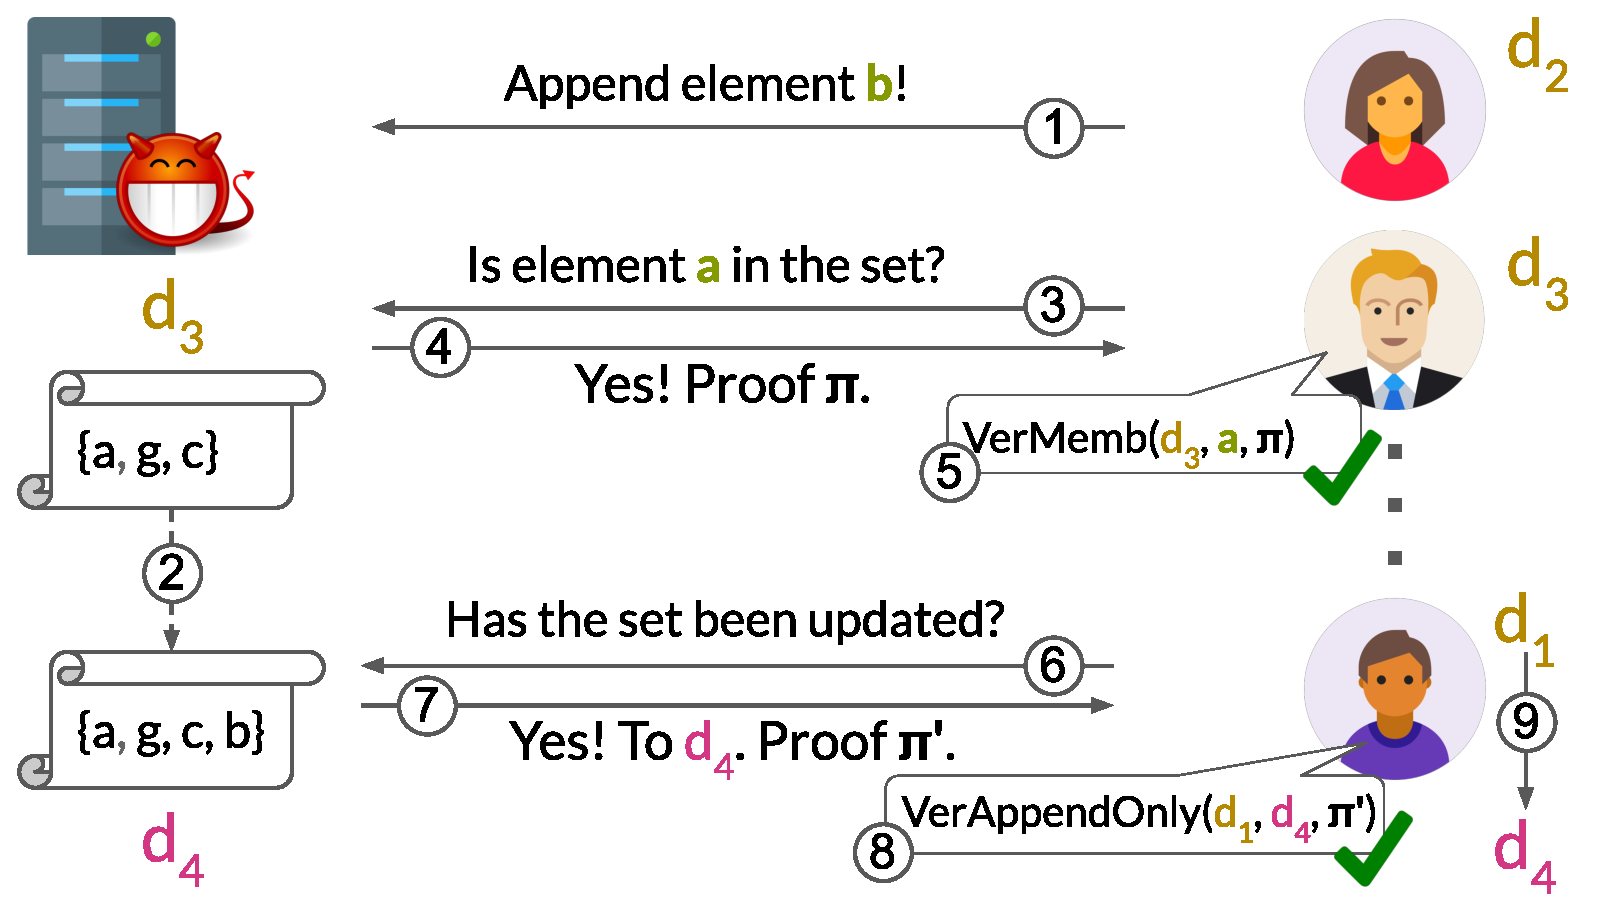
\includegraphics[width=1.0\columnwidth]{figures/model.pdf}
    \vspace{-.5cm}
    \caption{
        Our model: a single malicious \textit{server} manages a \textit{set} and many \textit{clients} query the set.
        Clients will not necessarily have the digest of the latest set.
        The clients can (1) append a new element to the set, (2) query for an element and (3) ask for an updated digest of the set.
    }
    \label{f:model}
    \vspace{-1.5em}
\end{figure}
}

\figModel

\section{Append-only Authenticated Sets}
\label{s:aas}

We begin by introducing a new primitive called an \textit{append-only authenticated set} (AAS).
An AAS can be used for Revocation Transparency (RT) as proposed by Google~\cite{rev-transparency}.
In \cref{s:aad}, we modify our AAS into an \textit{append-only authenticated dictionary} (AAD), which can be used for generalized transparency~\cite{general-transparency}.

\parhead{Overview.}
An AAS is a set of \textit{elements} managed by an \textit{untrusted server} and queried by \textit{clients}.
The server is the sole author of the AAS: it can append elements on its own and/or accept elements from clients.
% e.g., from History Tree paper: "Tamper-evident logs are fundamentally different: An untrusted logger is the sole author of the log and is responsible for both building and signing it.
% This is different from other models where elements might come from a \textit{trusted source} who signs them~\cite{two-party-ad,pads}.
Clients can check membership of elements in the set (see Steps 3-5 in \cref{f:model}).
Clients, also known as \textit{users}, are mutually-distrusting, potentially malicious, and do not have identities (i.e., no authorization or authentication).
Initially, the set starts out empty at \textit{version} zero, with new appends increasing its size and version by one.
Importantly, once an element has been appended to the set, it remains there forever: an adversary cannot remove nor change the element.
After each append, the server signs and publishes a new, small-sized \emph{digest} of the updated set (e.g., Step 2).

Clients periodically update their view of the set by requesting a new digest from the server (e.g., Step 6 and 7).
The new digest could be for an arbitrary version $j > i$, where $i$ is the previous version of the set (not just for $j = i+1$).
Importantly, clients always ensure the set remains \textit{append-only} by verifying an \textit{append-only proof} $\pi_{i,j}$ between the old and new digest (e.g., Step 8).
This way, clients can be certain the malicious server has not removed any elements from the set.
Clients will not necessarily have the latest digest of the set.
Finally, clients securely check if an element $k$ is in the set via a \emph{(non)membership proof} (e.g., Steps 3-5 in \cref{f:model}).

A malicious server can \emph{fork} clients' views~\cite{sundrosdi}, preventing them from seeing each other's appends.
To deal with this, clients maintain a \textit{fork consistent} view~\cite{beyondonethird,sundrosdi} of the set by checking append-only proofs.
As a consequence, if the server ever withholds an append from one client, that client's digest will forever diverge from other clients' digests.
To detect such \textit{forks}, clients can \textit{gossip}~\cite{ct-gossip,cosi,catena,DahlbergPullsVestin2018} with one another about their digests.
This is crucial for security in transparency logs.

This model is the same as in history trees (HTs)~\cite{ht}, assuming only a gossip channel and no trusted third parties.
It also arises in encrypted web applications~\cite{mylar,verena,frientegrity}, Certificate Transparency (CT)~\cite{ct} and software transparency schemes~\cite{at,chainiac}.
Unlike the 2- and 3-party models~\cite{two-party-ad,pads,balloon}, there is no \textit{trusted source} that signs appends in this model.
A trusted source trivially solves the AAS/AAD problem as it can simply vouch for the data structure's append-only property with a digital signature.
Unfortunately, this kind of solution is useless for transparency logs~\cite{ct,ect,coniks}, which lack trusted parties.

%\subsection{Append-only Authenticated Set API}

\parhead{Server-side API.}
The untrusted server implements:
\vspace{.5em}

\api {\setup}$(1^\lambda, \beta) \rightarrow pp, VK$.
Randomized algorithm that returns public parameters $pp$ used by the server and a \textit{verification key} $VK$ used by clients.
Here, $\lambda$ is a security parameter and $\beta$ is an upper-bound on the number of elements $n$ in the set (i.e., $n \le \beta$).

\api {\append}$(pp, \AS_i, d_i, k) \rightarrow \AS_{i+1}, d_{i+1}$.
Deterministic algorithm that appends a new element $k$ to the version $i$ set, creating a new version $i+1$ set.
Succeeds only if the set is not full (i.e., $i + 1 \le \beta$).
Returns the new authenticated set $\AS_{i+1}$ and its digest $d_{i+1}$.

\api $\provememb(pp, \AS_i, k) \rightarrow b, \pi$.
Deterministic algorithm that proves (non)membership for element $k$.
When $k$ is in the set, generates a membership proof $\pi$ and sets $b=1$.
Otherwise, generates a non-membership proof $\pi$ and sets $b=0$.

\api {\proveappendonly}$(pp, \AS_i, \AS_j) \rightarrow \pi_{i, j}$.
Deterministic algorithm that proves $\AS_i \subseteq \AS_j$.
In other words, generates an \textit{append-only proof} $\pi_{i, j}$ that all elements in $\AS_i$ are also present in $\AS_j$.
Importantly, a malicious server who removed elements from $\AS_j$ that were present in $\AS_i$ cannot construct a valid append-only proof.

\parhead{Client-side API.}
Clients implement:
\vspace{.5em}

\api {\vermemb}$(VK, d_i, k, b, \pi) \rightarrow \{T, F\}$.
Deterministic algorithm that verifies proofs returned by $\provememb(\cdot)$ against the digest $d_i$.
When $b=1$, verifies $k$ is in the set via the membership proof $\pi$.
When $b=0$, verifies $k$ is \textit{not} in the set via the non-membership proof $\pi$.
(We formalize security in \cref{s:aas:correctness-and-security}.)

\api {\verappendonly}$(VK, d_i, i, d_j, j, \pi_{i,j}) \rightarrow \{T, F\}$.
Deterministic algorithm that ensures a set remains append-only.
Verifies that $\pi_{i,j}$ correctly proves that the set with digest $d_i$ is a subset of the set with digest $d_j$.
Also, verifies that $d_i$ and $d_j$ are digests of sets at version $i$ and $j$ respectively, enforcing fork consistency.

\parhead{Using the API.}
To use an AAS scheme, first, public parameters need to be computed using a call to $\setup(\cdot)$.
If the AAS scheme is trapdoored, a trusted party or MPC protocol runs $\setup(\cdot)$ and forgets the trapdoor (see \cref{s:discussion}).
Once computed, the parameters can be reused by different servers for different append-only sets.
$\setup(\cdot)$ also returns a \textit{public} verification key $VK$ to all clients.

Then, the server broadcasts the initial digest $d_0$ of the empty set $\AS_0$ to its many clients.
Clients can concurrently start appending elements using $\append(\cdot)$ calls.
If the server is honest, it serializes $\append(\cdot)$ calls.
Eventually, the server returns a new digest $d_i$ to clients along with an append-only proof $\pi_{0,i}$ computed using $\proveappendonly(\cdot)$.
Some clients might be offline but eventually they will receive either $d_i$ or a newer $d_j, j > i$.
Importantly, whenever clients transition from version $i$ to $j$, they check an append-only proof $\pi_{i,j}$ using $\verappendonly(VK, d_i, i, d_j, j, \pi_{i,j})$.

Clients can look up elements in the set.
The server proves (non)\hyp{}membership of an element using $\provememb(\cdot)$.
A client verifies the proof using $\vermemb(\cdot)$ against their digest.
As more elements are added by clients, the server continues to publish a new digest $d_j$ and can prove it is a superset of any previous digest $d_i$ using $\proveappendonly(\cdot)$.

\subsection{AAS Correctness and Security Definitions}
\label{s:aas:correctness-and-security}
We first introduce some helpful notation for our correctness definitions.
Consider an ordered sequence of $n$ appends $(k_i)_{i\in [n]}$.
% NOTE: Can force \newline in inline equations but is there a better way?
% --- begin multiline ---
Let 
$\AS',d' \leftarrow \multiappend(pp, \AS, d, (k_i)_{i\in [n]})$ 
denote a sequence of $\append(\cdot)$ calls arbitrarily interleaved with other $\provememb(\cdot)$ and $\proveappendonly(\cdot)$ calls such that 
$\AS',d'$ $\leftarrow$ $\append(pp,\AS_{n-1}$, $d_{n-1}, k_{n})$,
$\AS_{n-1}, d_{n-1}$ $\leftarrow$ $\append(pp,\AS_{n-2}, d_{n-2}, k_{n-1})$,
$\dots$,
$\AS_{1}, d_1$ $\leftarrow$ $\append(pp,\AS, d, k_{1})$.
% --- end of multiline ---
Finally, let $\AS_0$ denote an empty AAS with empty digest $d_0$.

\begin{definition}[Append-only Authenticated Set]
    \label{d:secure-aas-definition}
    (\setup, \append, \provememb, \proveappendonly, \vermemb, \verappendonly) is a secure append-only authenticated set (AAS) if
    $\exists$ a negligible function $\negl$,
    $\forall$ security parameters $\lambda$,  $\forall$ upper-bounds $\beta=\poly(\lambda)$ and $\forall n \le \beta$ it satisfies the following properties:
\end{definition}

\parhead{Membership correctness.}
\label{s:aas:membership-correctness}
$\forall$ ordered sequences of appends $(k_i)_{i\in[n]}$, for all elements $k$, where $b=1$ if $k\in (k_i)_{i\in[n]}$ and $b=0$ otherwise,
\begin{align*}
\small
\Pr \left[ \begin{array}{c}
(pp,VK) \leftarrow \setup(1^\lambda, \beta),\\
(\AS, d) \leftarrow \multiappend(pp, \AS_0, d_0, (k_i)_{i\in[n]}),\\
(b',\pi) \leftarrow \provememb(pp,\AS, k): \\
{{b=b'}\wedge{\vermemb(VK, d, k, b, \pi) = T}}
\end{array} \right]
\ge 1 - \negl(\lambda)
\end{align*}

\noindent \textit{Observation:}
Note that this definition compares the returned bit $b'$ with the ``ground truth'' in $(k_i)_{i\in[n]}$ and thus provides membership correctness.
Also, it handles non-membership correctness since $b'$ can be zero.
Finally, the definition handles all possible orders of appending elements.

\parhead{Membership security.}
\label{s:aas:membership-security}
$\forall$ adversaries \textsf{A} running in time $\mathsf{poly}(\lambda)$,
\begin{align*}
\small
\Pr \left[ \begin{array}{c}
(pp,VK) \leftarrow \setup(1^\lambda, \beta), \\
(d, k,\pi,\pi') \leftarrow \mathsf{A}(pp, VK)
: \\
{\vermemb(VK,d, k,0,\pi ,) = T} \wedge {} \\
{\vermemb(VK,d, k,1,\pi',) = T}
\end{array} \right] \le \negl(\lambda)
\end{align*}

\noindent \textit{Observation:}
This definition captures the lack of any ``ground truth'' about what was inserted in the set, since there is no trusted source in our model.
Nonetheless, given a fixed digest $d$, our definition prevents \textit{all} equivocation attacks about the membership of an element in the set.
% Note that this definition implies that different sets cannot have the same digest.
% Suppose you have two different sets with the same digest.
% Then membership correctness says you can create proofs for all elements that pass verification.
% Since the sets differ, there exists an element $x$ that is in one set but not the other.
% Yet we will have both membership and non-membership proofs of $x$ that verify w.r.t. the same digest.
% But this breaks membership security. Contradiction.

\parhead{Append-only correctness.}
\label{s:aas:appendonly-correctness}
$\forall m < n,\forall$ sequences of appends $(k_i)_{i\in[n]}$ where $n\ge2$,
\begin{align*}
\small
\Pr \left[ \begin{array}{c}
(pp,VK) \leftarrow \setup(1^\lambda, \beta) \\
(\AS_m, d_m) \leftarrow \multiappend(pp,\AS_0,d_0,(k_i)_{i\in[m]}),\\
(\AS_n, d_n) \leftarrow \multiappend(pp,\AS_m,d_m,(k_i)_{i\in[m+1,n]}),  \\
\pi \leftarrow \proveappendonly(pp,\AS_m, \AS_n):\\
{\verappendonly(VK, d_m, m, d_n, n, \pi) = T}
\end{array} \right] \ge 1 - \negl(\lambda)
\end{align*}

\parhead{Append-only security.}
\label{s:aas:appendonly-security}
$\forall$ adversaries \textsf{A} running in time $\mathsf{poly}(\lambda)$,
\begin{align*}
\small
\Pr \left[ \begin{array}{c}
(pp,VK) \leftarrow \setup(1^\lambda, \beta)\\
(d_i,d_j,i < j,\pi_a, k,\pi,\pi') \leftarrow \mathsf{A}(pp, VK)
: \\
{\verappendonly(VK, d_i, i, d_j, j, \pi_a) = T} \wedge {}\\
{\vermemb(VK, d_i, k, 1, \pi )  = T} \wedge {}\\
{\vermemb(VK, d_j, k, 0, \pi') = T}
\end{array} \right] \le \negl(\lambda)
\end{align*}

\noindent \textit{Observation:}
This definition ensures that elements can only be added to an AAS.

\parhead{Fork consistency.}
\label{s:aas:fork-consistency}
$\forall$ adversaries \textsf{A} running in time $\mathsf{poly}(\lambda)$,
\begin{align*}
\Pr \left[ \begin{array}{c}
(pp,VK) \leftarrow \setup(1^\lambda, \beta)\\
(d_i\ne d_i',d_j,i<j,\pi_i,\pi_i') \leftarrow \mathsf{A}(pp, VK)
: \\
{\verappendonly(VK, d_i , i, d_j, j, \pi_i) = T} \wedge {}\\
{\verappendonly(VK, d_i', i, d_j, j, \pi_i') = T}\\
\end{array} \right] \le \negl(\lambda)
\end{align*}

\noindent \textit{Observation:}
This is our own version of fork consistency that captures what is known in the literature about fork consistency~\cite{ht,beyondonethird}.
Specifically, it allows a server to fork the set at version $i$ by presenting two different digests $d_i$ and $d_i'$ and prevents the server from forging append-only proofs that ``join'' the two forks into some common digest $d_j$ at a later version $j$.

  % FIXED
\section{AAS from Accumulators}
\label{s:aas:construction}

This section presents our accumulator-based AAS construction.
We focus on bilinear accumulators here and discuss how our construction would benefit from RSA accumulators in \cref{s:aas:rsa}.
We give a more formal algorithmic description in \cref{s:aas:algorithms}.

As mentioned in \cref{s:intro:overview-techniques}, a bilinear accumulator over $n$ elements is already an AAS, albeit an inefficient one.
Specifically, proving (non)membership in a bilinear accumulator requires an $O(n)$ time polynomial division.
As a consequence, precomputing all $n$ membership proofs (naively) takes $O(n^2)$ time, which is prohibitive for most use cases.
Even worse, for non-membership, one must precompute proofs for all possible missing elements, of which there are exponentially many (in the security parameter $\lambda$).
Therefore, we need new techniques to achieve our desired polylogarithmic time complexity for computing both types of proofs in our AAS.

\parhead{A bilinear tree accumulator.}
Our first technique is to deploy the bilinear accumulator in a tree structure, as follows.
We start with the elements $e_i$ as leaves of a binary tree (see \cref{f:accumulated-tree}b).
Specifically, each leaf will store an accumulator over the singleton set $\{e_i\}$.
Every internal node in the tree will then store an accumulator over the union of the sets corresponding to its two children.
For example, the parent node of the two leaves corresponding to $\{e_i\}$ and $\{e_{i+1}\}$ stores the accumulator of the set $\{e_i,e_{i+1}\}$.
In this way, the root is the accumulator over the full set $S = \{e_1,\dots,e_n\}$ (see \cref{f:accumulated-tree}).
We stress that all these accumulators use the same public parameters.
The time to compute all the accumulators in the tree is $T(n) = 2T(n/2) + O(n\log{n}) = O(n\log^2{n})$ where $O(n\log{n})$ is the time to multiply the characteristic polynomials of two sets of size $n$ in the tree.
We call the resulting structure a \emph{bilinear tree} over set $S$.

\begin{figure}[t]
    \centering
    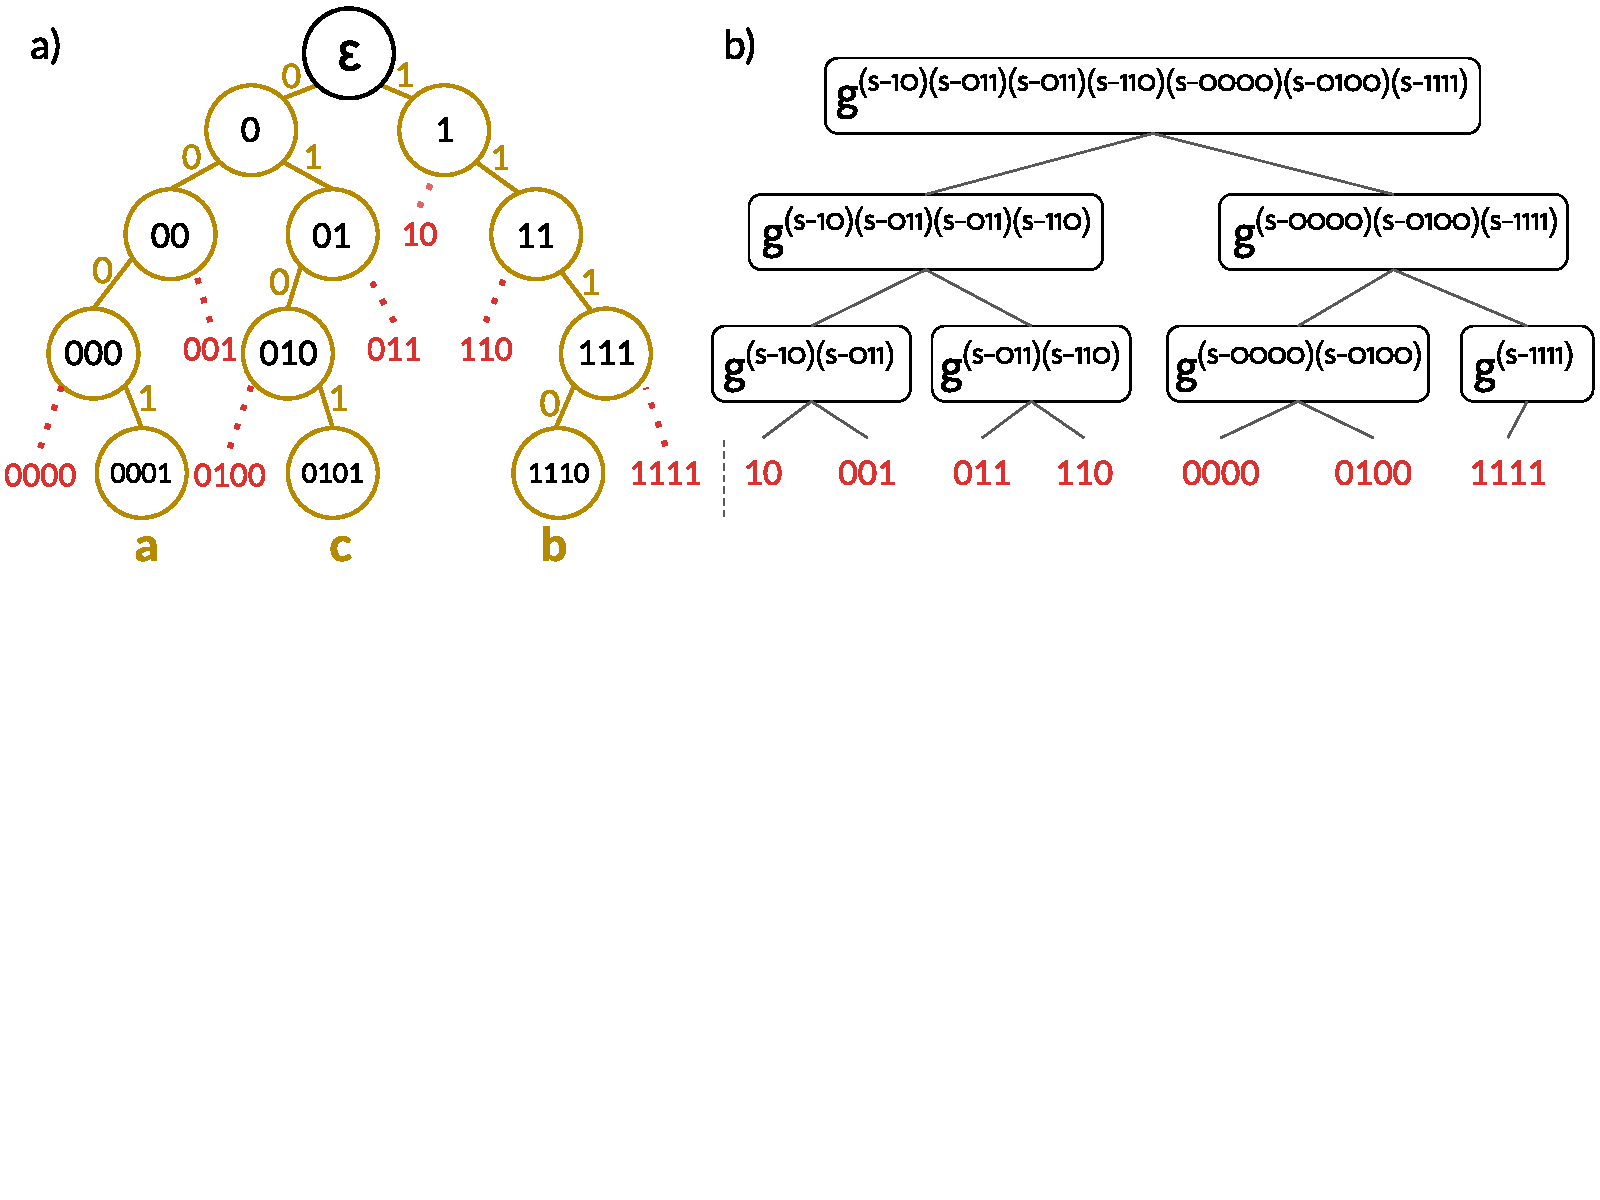
\includegraphics[width=1.00\columnwidth]{figures/AT.pdf}
    \vspace{-4.0cm}
    \caption{
        On the left side, we depict a trie over set $S = \{a,b,c\}$.
        Each element is mapped to a unique path of length $4$ in the trie.
        Nodes that are not in the trie but are at its \textit{frontier} are depicted in \myred{\textbf{red}}.
        On the right side, we depict a \textit{bilinear frontier tree} (BFT) corresponding to the set $S$.
        To prove that an element is not in $S$, we prove one of its prefixes is in the BFT.
        \label{f:accumulated-tree}}
    \vspace{-2.5em}
\end{figure}

\parhead{Membership proofs in bilinear trees.}
A membership proof for element $e_i$ will leverage the fact that sets along the path from $e_i$'s leaf to the root of the bilinear tree are subsets of each other.
The proof will consist of a sequence of \textit{subset proofs} that validate this (computed as explained in \cref{s:prelim:polycommit}).
Specifically, the proof contains the accumulators along the path from $e_i$'s leaf to the root, as well as the accumulators of all sibling nodes along this path (see \cref{f:accumulated-tree}b).
The client verifies all these subset proofs, starting from the singleton set $\{e_i\}$ in the leaf.
This convinces  him that $e_i$ is contained in the parent's accumulated set, which in turn is contained in its parent's accumulated set and so on, until the root.

Our bilinear tree approach gives us membership proofs of logarithmic size and thus logarithmic verification time.
Importantly, computing a bilinear tree in $O(n\log^2{n})$ time implicitly computes all membership proofs ``for free''!
In contrast, building a standard billinear accumulator over $S$ would yield constant-size proofs but in $O(n^2)$ time for all $n$ proofs.
Unfortunately, our bilinear tree structure does not (yet) support precomputing non-membership proofs.
We devise new techniques that address this next.

\parhead{Bilinear prefix trees to the rescue.}
To efficiently precompute non-membership proofs, we slightly modify our bilinear tree.
Instead of storing an element $e_i \in S$, the $i$th leaf will store the \emph{set of prefixes} of the binary representation of $e_i$.
We assume this representation is $2\lambda$ bits (or is made so using a CRHF) and can be mapped to an element in $\Fp$ (which is also of size $\approx 2\lambda$ bits) and thus can be accumulated.
For example, a leaf that previously stored element $e_1$ with binary representation $0001$, will now store the set $P(e_1) = \{\varepsilon,0,00,000,0001\}$ (i.e., all the prefixes of the binary representation of $e_1$, including the empty string $\varepsilon$).
In general, for each element $e_i$, $P(e_i)$ is the set of all $2\lambda+1$ prefixes of $e_i$.
Also, for any set $S = \{e_1,\dots,e_n\}$, we define its \emph{prefix set} as $P(S) = P(e_1) \cup \dots \cup P(e_n)$.
For example, let $S =\{a=0001,b=0101,c=1110\}$.
The root of $S$'s bilinear tree will contain an accumulator over $P(S) = P(a) \cup P(b) \cup P(c) = \{\varepsilon,0,1,00,01,11,000,010,111,0001,0101,1110\}$.

We refer to such a bilinear tree as a \emph{bilinear prefix tree (BPT)} over $S$.
The time to build a BPT for $S$ is $O(\lambda n\log^2{n})$ since there are $O(\lambda n)$ prefixes across all leaves.
Note that membership proofs in a BPT are the same as in bilinear trees, with a minor change.
The internal nodes of the tree still store accumulators over the union of their children.
However, the children now have common prefixes, which will only appear once in the parent.
For example, two children sets have the empty string $\varepsilon$ while their parent set only has $\varepsilon$ once (because of the union).
As a result, it is no longer the case that multiplying the characteristic polynomials of the children gives us the parent's polynomial.
Therefore, we can no longer rely on the siblings as subset proofs: we have to explicitly compute subset proofs for each child w.r.t. its parent.
We stress that this does not affect the asymptotic time complexity of computing the BPT.
As before, the client starts the proof verification from the leaf, which now stores a prefix set $P(e_i)$ rather than a singleton set $\{e_i\}$.

\begin{figure}[t]
    \centering
    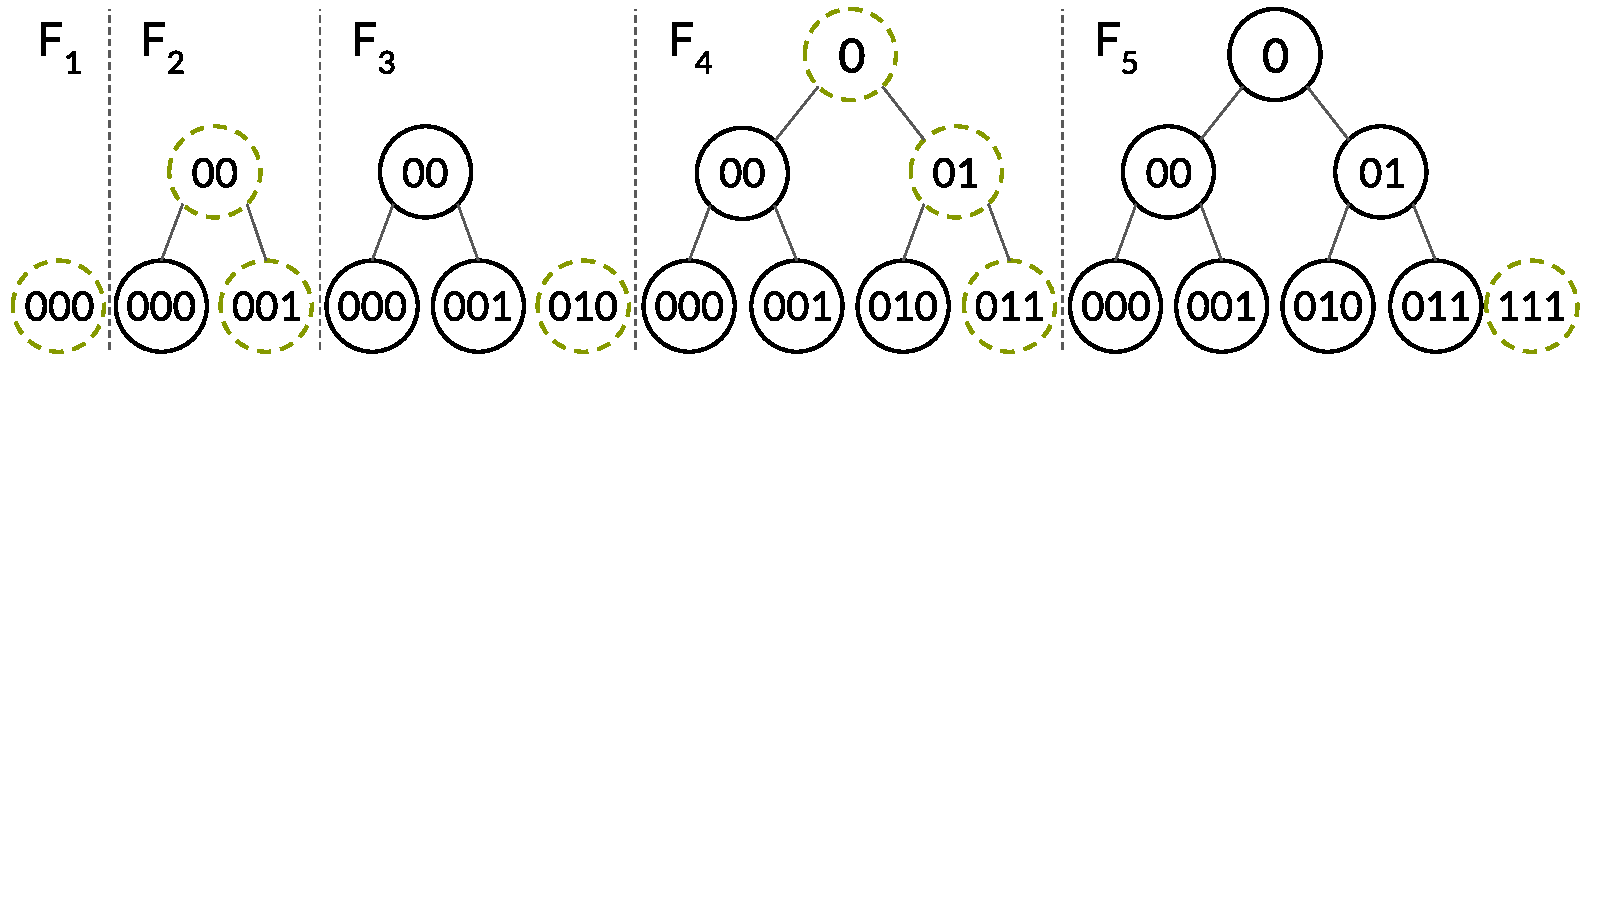
\includegraphics[width=1\columnwidth]{figures/forest.pdf}
    \vspace{-3.4cm}
    \caption{
        A forest starting empty and going through a sequence of five appends.
        A forest only has trees of exact size $2^j$ for distinct $j$'s.
        A forest of $n$ leaves has \textit{at most} $\log{n}$ trees. 
    }
    \label{f:forest}
    \vspace{-1.55em}
\end{figure}

\parhead{Efficient non-membership proofs.}
But how does a BPT help with precomputing non-membership proofs for any element $e'\notin S$?
First, note that, because of our use of prefixes, to prove $e'\notin S$ it suffices to show that \textit{any one prefix $\rho$ of $e'$ is not contained in $P(S)$}.
Second, note that there might exist other elements $e''$ who share $\rho$ as a prefix.
As a result, the non-membership proof for $e'$ could be ``reused'' as a non-membership proof for $e''$.
This is best illustrated in \cref{f:accumulated-tree}a using our previous example where $S =\{a,b,c\}$.
Consider elements $d= \underline{011}1$ and $f = \underline{011}0$ that are not in $S$.
To prove non-membership for either element, it suffices to prove the same statement: $\underline{011}\notin P(S)$.
Thus, if we can identify all such \textit{shared prefixes}, we can use them to prove the non-membership of (exponentially) many elements.
(This technique is also used in Micali et al.'s zero-knowledge sets~\cite{zks}.)

To do this, we insert all elements from $S$ in a trie as depicted in \cref{f:accumulated-tree}a.
Next, we keep track of the prefixes at the ``frontier'' of the trie depicted in red in \cref{f:accumulated-tree}a.
We immediately notice that to prove non-membership of any element, it suffices to prove non-membership of one of these \textit{frontier prefixes}!
In other words, elements that are not in $S$ will have one of these as a prefix.
Thus, we formally define the \textit{frontier} of $S$ as:
\begin{align*}
    F(S) &= \{\rho \in \{0,1\}^{\le 2\lambda}: {\rho\not \in P(S)} \wedge {\parent(\rho) \in P(S)}\}\text{,}
\end{align*}
where $\parent(\rho)$ is $\rho$ without its last bit (e.g., $\parent(011) = 01$).
Note that the size of $F(S)$ is $O(\lambda n)$, proportionate to $P(S)$.

Most importantly, from the way $P(S)$ and $F(S)$ are defined, for any element $e'$ it holds that $e'\not\in S$ if, and only if, some prefix of $e'$ is in $F(S)$. 
Therefore, proving non-membership of $e'$ boils down to proving two statements: (i) some prefix of $e'$ belongs to $F(S)$, and (ii) $P(S) \cap F(S) = \varnothing$.
We stress that the latter is necessary as a malicious server may try to craft $F(S)$ in a false way (e.g., by adding some prefixes both in $P(S)$ and in $F(S)$).
To prove (i), we build a bilinear tree over $F(S)$ which gives us precomputed membership proofs for all $\rho \in F(S)$.
We refer to this tree as the \emph{bilinear frontier tree (BFT)} for set $S$ and to the proofs as \textit{frontier proofs}.
To prove (ii), we compute a \emph{disjointness proof} between sets $P(S)$ and $F(S)$, as described in \cref{s:prelim:polycommit} (i.e., between the root accumulators of the BFT and the BPT of $S$).
The time to build a BFT for $S$ is $O(\lambda n\log^2{n})$ since $F(S)$ has $O(\lambda n)$ elements.
The disjointness proof can be computed in $O(\lambda n\log^2{n})$ time. 

\parhead{Static AAS construction.}
Combining all the above techniques, we obtain a \textit{static} AAS that does not support updates efficiently (nor append-only proofs).
This construction consists of: (a) a BPT for $S$, (b) a BFT for $S$, and (c) a proof of disjointness between $P(S)$ and $F(S)$ (i.e., between the root BPT and BFT accumulators).
The height of the BPT is $O(\log n)$ and the height of the BFT is $O(\log{(\lambda n)})$ so the size and verification time of a (non)membership proof is $O(\log{n})$.
The digest is just the root accumulator of the BPT. 

\begin{figure}[t]
    \centering
    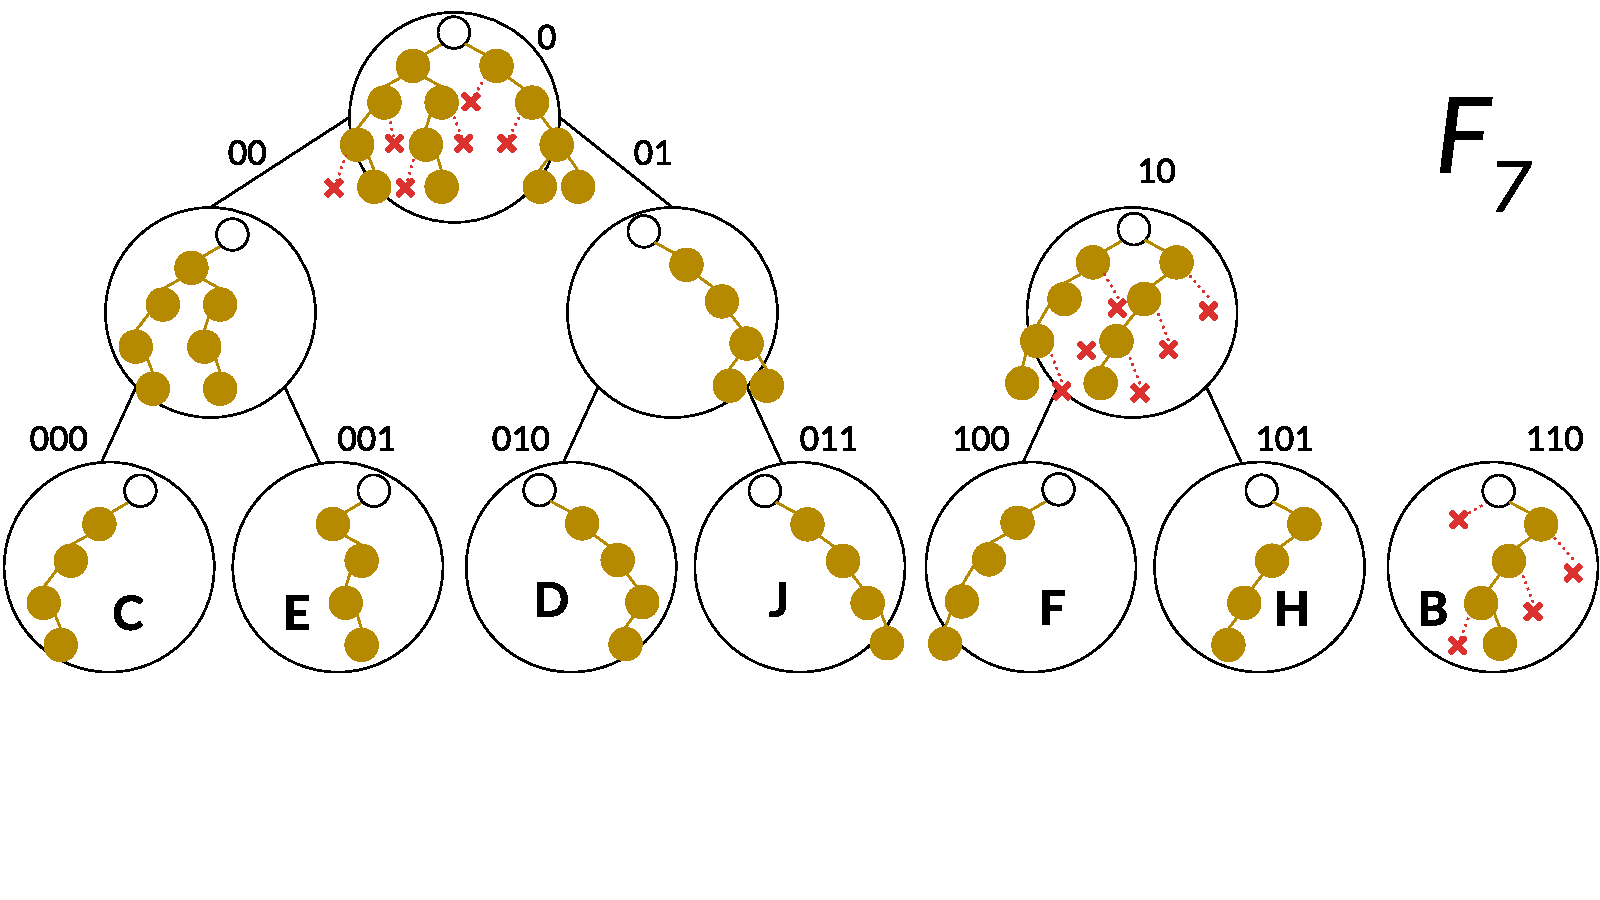
\includegraphics[width=1.00\columnwidth]{figures/accaad.pdf}
    \vspace{-1.7cm}
    \caption{
        A dynamic AAS with $\lambda=2$ for set $\{B,C,D,E,F,H,J\}$.
        Our AAS is a forest of BPTs with corresponding BFTs.
        Each node stores a BPT accumulator (and subset proof), depicted as a trie, in \myyellow{yellow}.
        Root nodes store a BFT, depicted as the missing \myred{red} nodes.
    }
    \vspace{-1.9em}
    \label{f:accaas}
\end{figure}

\parhead{Handling appends efficiently.}
So far, we only discussed the case of a static set $S$.
However, our AAS should support appending new elements to $S$. 
The main challenge here is \emph{efficiency} since updating the BPT and BFT as well as the disjointness proof after each update is very expensive (at least linear).
To address this we use a classic ``amortization'' trick from Overmars~\cite{overmars} also used in~\cite{distributed-acc}. 

Specifically, our AAS will consist not of one BPT for the entire set $S$, but will be partitioned into a \textit{forest} of BPTs and their corresponding BFTs.
Initially, we start with no elements in the AAS.
When the first element $e_1$ is appended, we build its \textit{tree-pair}: a BPT over the set $\{e_1\}$, its BFT and a disjointness proof.
When the second element $e_2$ is appended, we ``merge'': we build a size-2 tree-pair over $\{e_1, e_2\}$.
The rule is we always merge equal-sized tree-pairs.
When $e_3$ is appended, we cannot merge it because there's no other tree-pair of size 1.
Instead, we create a tree-pair over $\{e_3\}$.
In general, after $2^\ell - 1$ appends, we end up with $\ell$ separate tree-pairs corresponding to sets of elements $S_1,\dots,S_\ell$.
The final set is $S=\bigcup_{j=1}^{\ell} S_j$ where $|S_j| = 2^j$.
The evolution of such a forest is depicted in \cref{f:forest} and the final data structure can be seen in \cref{f:accaas}.

Let us analyze the time to merge two size-$n$ tree-pairs for $S_1$ and $S_2$ into a size-$2n$ tree-pair for $S=S_1 \cup S_2$.
To compute $S$'s BPT, we need to (i) compute its root accumulator, (ii) set its children to the ``old'' root accumulators of $S_1$ and $S_2$ and (iii) compute subset proofs $S_1 \subset S$ and $S_2\subset S$.
Since $|S_1|=|S_2|=n$, operations (i), (ii) and (iii) take $O(\lambda n \log^2{n})$ time.
Finally, we can compute $S$'s BFT from scratch in $O(\lambda n\log^2 n)$ time.

To analyze the append time, consider the time $T(n)$ to create an AAS over a set $S$ with $n = 2^\ell$ elements (without loss of generality).
Then, $T(n)$ is just the time to create a tree-pair over $S$ and can be broken into (i) the time to create a tree-pair over the children of $S$ of size $n/2$ (i.e., $2T(n/2)$) (ii) the time to merge these two children BPTs (including computing subset proofs) and (iii) the time to compute the BFT of $S$.
More formally, $T(n) = 2T(n/2) + O(\lambda n\log^2{n})$ which simplifies to $T(n) = O(\lambda n\log^3{n})$ time for $n$ appends.
Thus, the \textit{amortized} time for one append is $O(\lambda \log^3 {n})$ and can be de-amortized into \textit{worst-case} time using generic techniques~\cite{overmars,overmars-van-leeuwen}.

The downside of our amortized approach is that proving non-membership becomes slightly more expensive than in the static AAS data structure from above.
Specifically, now the server needs to prove non-membership in each tree-pair separately, requiring an $O(\log{n})$ frontier proof in each of the $O(\log{n})$ BFTs.
This increases the non-membership proof size to $O(\log^2 n)$.
On a good note, membership proofs remain unaffected: the server just sends a path to a leaf in \textit{one} of the BPTs where the element is found.
Finally, the AAS digest is set to the root accumulators of all BPTs and has size $O(\log{n})$.
We analyze the complexity of our AAS in \cref{s:aas:asymptotics}.

\parhead{Efficient append-only proofs.}
Our append-only proofs are similar to the ones in history trees~\cite{ht}.
% Recall that when we merge the BPTs for $S_1, S_2$ and build a new BPT, (i) we compute its new root as the accumulator of $P(S_1) \cup P(S_2)$, (ii) we set the two old roots as the new root's children and (iii) we compute subset proofs between the old roots and the new root.
% Thus, the old roots become children nodes in the new BPT.
% In fact, because every append to the AAS triggers a sequence of merges, we can generalize the above statement: after a sequence of appends, \textit{some} of the old roots in the old AAS will become descendants of a new root in the new AAS.
% The remaining old roots, if any, will remain as (new) roots in the new forest (e.g., root 0 from $F_4$ to $F_5$ in \cref{f:forest}).
% Our append-only proof leverages the above invariant.
An append-only proof must relate the root BPT accumulator(s) in the old AAS to the root BPT accumulator(s) in the new AAS.
We'll refer to these as ``old roots'' and ``new roots'' respectively.
Specifically, it must show that every old root either (i) became a new root or (ii) has a path to a new root with valid subset proofs at every level.
Such a path is verified by checking the subset proofs between every child and its parent, exactly as in a membership proof.
At the same time, note that there might be new roots that are neither old roots nor have paths to old roots (e.g., root 111 in $F_5$ from \cref{f:forest}).
The proof simply ignores such roots since they securely add new elements to the set.
To summarize, the append-only proof guarantees that each old root (1) has a valid subset path to a new root or (2) became a new root.

\parhead{Ensuring fork-consistency.}
For gossip protocols to work~\cite{ct-gossip,DahlbergPullsVestin2018}, our AAS must be fork-consistent.
Interestingly, append-only proofs do not imply fork-consistency.
For example, consider a server who computes an AAS for set $\{e_1\}$ and another one for the set $\{e_2\}$. 
The server gives the first set's digest to user $A$ and the second digest to user $B$.
Afterwards, he appends $e_2$ to the first set and $e_1$ to the second one, which ``joins'' the two sets into a common set $\{e_1,e_2\}$.
The append-only property was not violated (as the two users can deduce independently) but fork-consistency has been: the two users had diverging views that were subsequently merged.

To avoid this, we will ``Merkle-ize'' each BPT using a CRHF $\Hb$ in the standard manner (i.e., a node hashes its accumulator and its two children's hashes).
Our AAS digest is now set to the Merkle roots of all BPTs, which implicitly commit to all root accumulators in the BPTs.
As a result, after merging BPTs for elements $e_1$ and $e_2$, the Merkle root of the merged BPT will differ based on how appends were ordered: $(e_1,e_2)$, or $(e_2,e_1)$.
Thus, violating fork-consistency becomes as hard as finding a collision in $\Hb$ (see \cref{s:aas:proofs:fork-consistency}).

  % FIXED
\section{From Sets to Dictionaries}
\label{s:aad}
In this section, we turn our attention to constructing an append-only authenticated dictionary (AAD).
Recall that an AAS stores \textit{elements} and supports (non)membership queries of the form ``Is $e\in S$?''
In contrast, an AAD stores \textit{key-value pairs} and supports \textit{lookups} of the form ``Is $V$ the complete set of values for key $k$?''
In other words, an AAD maps a \textit{key} $k$ to a multiset of \textit{values} $V$ in an append-only fashion.
Specifically, once a value has been added to a key, it cannot be removed nor changed.
For example, if a key is a domain name and its values are certificates for that domain, then an AAD can be used as a Certificate Transparency (CT) log.
In general, keys and values can have any application-specific type, as long as they can be hashed to a bit string.

Our construction  has great similarities with the AAS of \cref{s:aas:construction}.
However, the different functionality calls for modifications. 
Indeed, even the security notion for AADs is different (see \cref{s:prelim:notation:dictionaries}).
Specifically, in an AAS, no malicious server can simultaneously produce accepting proofs of membership and non-membership for the same element $e$ with respect to the same digest.
In contrast, in an AAD, no malicious server can simultaneously produce accepting proofs for two different sets of values $V,V'$ for a key $k$ with respect to the same digest.
This captures the related notion for an AAS since one of the sets of values may be empty (indicating $k$ has never been registered in the dictionary) and the other non-empty.
Next, we describe how we modify our AAS from \cref{s:aas:construction} to get an AAD.

\parhead{Encoding key-value pairs.}
An AAS construction can trivially support key-value pairs $(k,v)$ by increasing the size of the domain of the underlying AAS from $2\lambda$ bits to $4\lambda$ bits so as to account for the value $v$. 
That is, $(k,v)$ would be inserted in the AAS as $k|v$, using the same algorithms from \cref{s:aas:algorithms}.
Thus AAD clients now have twice the number of public parameters: $g^\tau, (g^{s^i})_{i=0}^{4\lambda+1}$.

\parhead{Proving lookups.}
For simplicity, let us restrict ourselves to an AAD of size $2^i$ (i.e., with just \textit{one} tree-pair).
For a key $k$ with no values, a lookup proof is simply a frontier proof for a prefix of $k$ in the BFT, much like a non-membership proof in the AAS (see \cref{s:aas:construction}).
What if $k$ has one or more values?
First, the lookup proof contains paths to BPT leaves with $k$'s values (i.e., with elements of the form $k|v$), much like a membership proof in an AAS.
But what is to guarantee \textit{completeness} of the response?
What if a malicious server leaves out one of the values of key $k$?
(This is important in transparency logs where users look up their own PKs and must receive all of them to detect impersonation attacks.)
We use the same frontier technique as in the AAS to convince clients values are not being left out.
Specifically, the server proves specific prefixes for the \textit{missing values} of $k$ are not in the BPTs (and thus are not maliciously being left out).
This is best illustrated with an example.

Suppose the server wants to prove $k=0000$ has \textit{complete} set of values $V=\{v_1 = 0001, v_2 = 0011\}$.
Consider a trie over $k|v_1$ and $k|v_2$ and note that $F^{[k]} = \{(0000|1), (0000|01), (0000|0000)$, $(0000|0010)\}$ is the set of all frontier prefixes for the missing values of $k$.
We call this set the \textit{lower frontier} of $k$ relative to $V$.
The key idea to prove completeness is to prove all lower frontier prefixes are in the BFT via frontier proofs (as discussed in \cref{s:aas:construction}).
Note that $|F^{[k]}| = O(\lambda)$ and each frontier proof is $O(\log{n})$-sized, resulting in an $O(\lambda \log{n})$-sized proof.
This idea generalizes to AADs of arbitrary size: the server (i) proves non-membership of $k$ in BPTs with no values for $k$ (via the BFT) and (ii) proves $V_i$ is the complete set of values of $k$ in each remaining BPT $i$ (via the BFT lower frontier technique).
In that case, a lookup proof for a key $k$ with a single value $v$ consists of (1) an $O(\log{n})$-sized path in some BPT with an $O(\lambda\log{n})$-sized frontier proof in its corresponding BFT (to guarantee completeness) and (2) an $O(\log{n})$-sized frontier proof for $k$ in all other $O(\log{n})$ BFTs, to prove $k$ has no values there.

\parhead{Smaller lookup proofs.}
When $k$ has one value, it follows from above that a lookup proof for $k$ is $O(\lambda \log{n})$-sized.
However, we can easily decrease its size to $O(\log^2{n})$.
Note that the main overhead comes from having to prove that all $O(\lambda)$ lower frontier prefixes of $k$ are in a BFT.
The key idea is to group all of $k$'s lower frontier prefixes into a single BFT leaf, creating an accumulator over all of them.
As a result, instead of having to send $O(\lambda)$ frontier proofs (one for each lower frontier prefix), we send a single $O(\log{n})$-sized frontier proof for a single BFT leaf which contains all lower frontier prefixes of $k$.
We can generalize this idea: when $k$ has $|V_i|$ values in the $i$th BFT in the forest, $k$'s lower frontier relative to $V_i$ has $O(|V_i|\lambda)$ prefixes.
Then, for each BFT $i$, we split the lower frontier prefixes of $k$ associated with $V_i$ into separate BFT leaves each of size at most $4\lambda + 1$.
We remind the reader that clients have enough public parameters  $(g^{s^i})_{i=0}^{4\lambda+1}$ to reconstruct the accumulators in these BFT leaves and verify the frontier proof.

\parhead{Supporting large domains and multisets.}
To handle keys and values longer than $2\lambda$ bits, we store $\mathcal{H}(k)|\mathcal{H}(v)$ in the AAD (rather than $k|v$), where $\mathcal{H}$ is a CRHF and we can retrieve the actual value $v$ from another repository.
To support multisets (same $v$ can be inserted twice for a $k$), the server can insert $\mathcal{H}(\mathcal{H}(v)|i)$ for the $i$-th occurrence of $(k,v)$.
% Simply inserting H(k)|H(v) does not work because if you insert (k,v) twice, and both insertions end up in the same BPT, then the frontier cannot be used to guarantee all copies of the same value $v$ have been revealed by the prover.
% In fact, the frontier is not even used here: the prover just gives a path to one of the (k,v)'s and then uses the frontier to show that there are not other values other than v for k in this BPT.
% The problem is that while that might be true, it does not say anything about how many times the value v occurrs in the BPT.

\parhead{Supporting inclusion proofs.}
Another useful proof for a transparency log is an \textit{inclusion proof} which only returns \textit{one of the values} of key $k$ (while lookup proofs return \textit{all} values of a key $k$).
For example, in Certificate Transparency (CT), browsers are supposed to verify an inclusion proof of a website's certificate before using it.
Our AAD supports inclusion proofs too.
They consist of a path to a BPT leaf with the desired key-value pair.
Since they do not require frontier proofs, inclusion proofs are only $O(\log{n})$-sized.
  % FIXED
\section{Evaluation}
\label{s:eval}

In this section, we evaluate our AAD (not AAS) construction's proof sizes, append times and memory usage.
We find that append times and memory usage are too high for a practical deployment and discuss how they might be improved in future work (see \cref{s:eval:append-time,s:eval:memory}).
If they are improved, we find AADs can save bandwidth relative to CT and CONIKS and we describe exactly when and how much in ~\cref{s:eval:worth-it}.

\parhead{Codebase and testbed.}
We implemented our \textit{amortized} AAD construction from \cref{s:aad} in 5700 lines of C++.
Its \textit{worst-case} append time is $O(\lambda n \log^2{n})$ while its amortized append time is $O(\lambda \log^3{n})$.
We used Zcash's \texttt{libff}~\cite{libff} as our elliptic curve library with support for a 254-bit Barretto-Naehrig curve with a Type~III pairing~\cite{bn-curve}.
% 110 bits for BN254: https://eprint.iacr.org/2016/1102.pdf
We used \texttt{libfqfft}~\cite{libfqfft} to multiply polynomials and \texttt{libntl}~\cite{libntl} to divide polynomials and compute GCDs.
Our code is available at:
\begin{center}
    \url{https://github.com/alinush/libaad-ccs2019}.
\end{center}
We ran our evaluation in the cloud on Amazon Web Services (AWS) on a r4.16xlarge instance type with 488 GiB of RAM and 64 VCPUs, running Ubuntu 16.04.4 (64-bit).
This instance type is ``memory-optimized'' which, according to AWS, means it is ``designed to deliver fast performance for workloads that process large data sets in memory.''

\begin{figure*}
\centering
\subfloat[Lookup proof (worst-case AAD sizes)]{\label{f:lookup-worst}%
    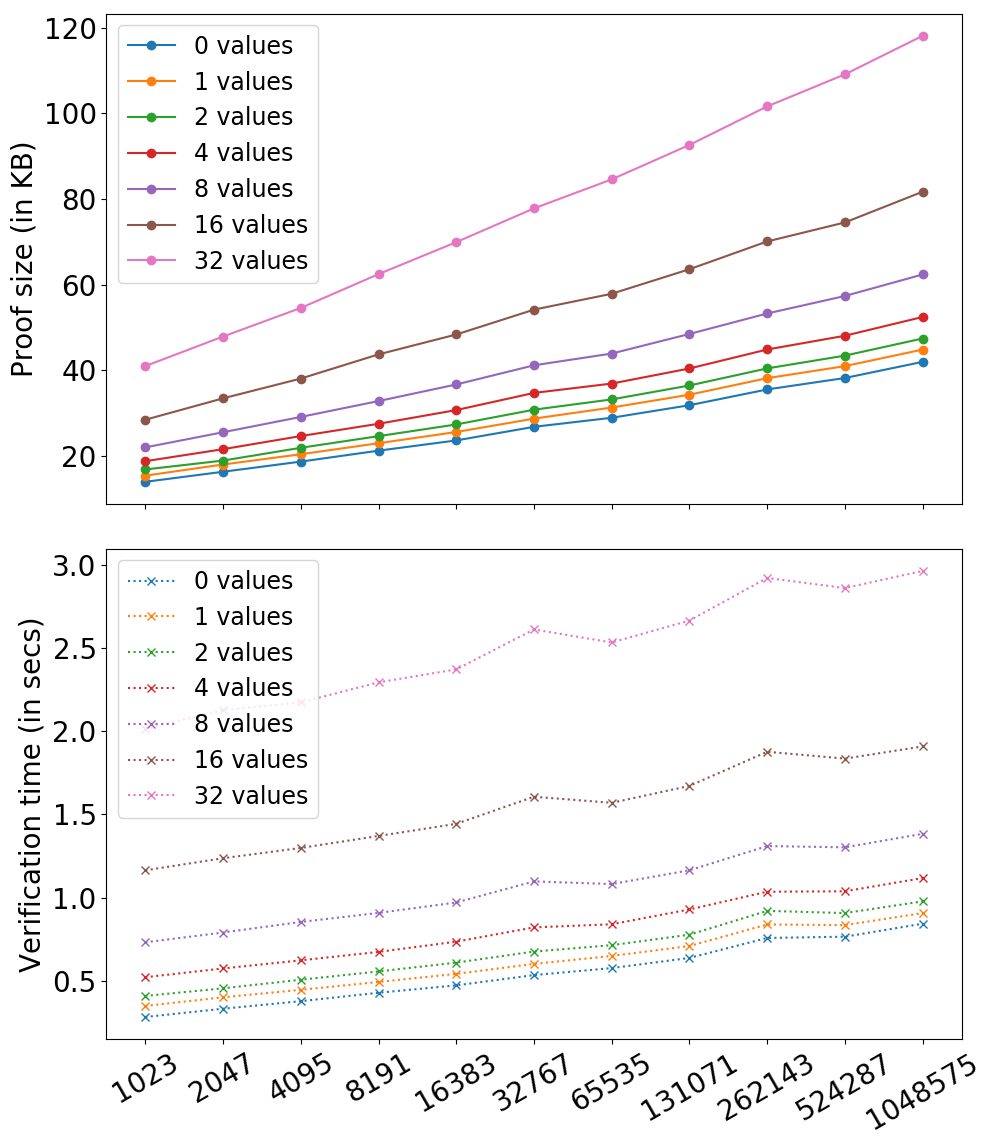
\includegraphics[width=0.32\linewidth]{figures/aad-memb-worst-case.png}
    \label{f:evaluation:lookup-worst}
}
\subfloat[Lookup proof (average-case AAD sizes)]{\label{f:lookup-avg}%
    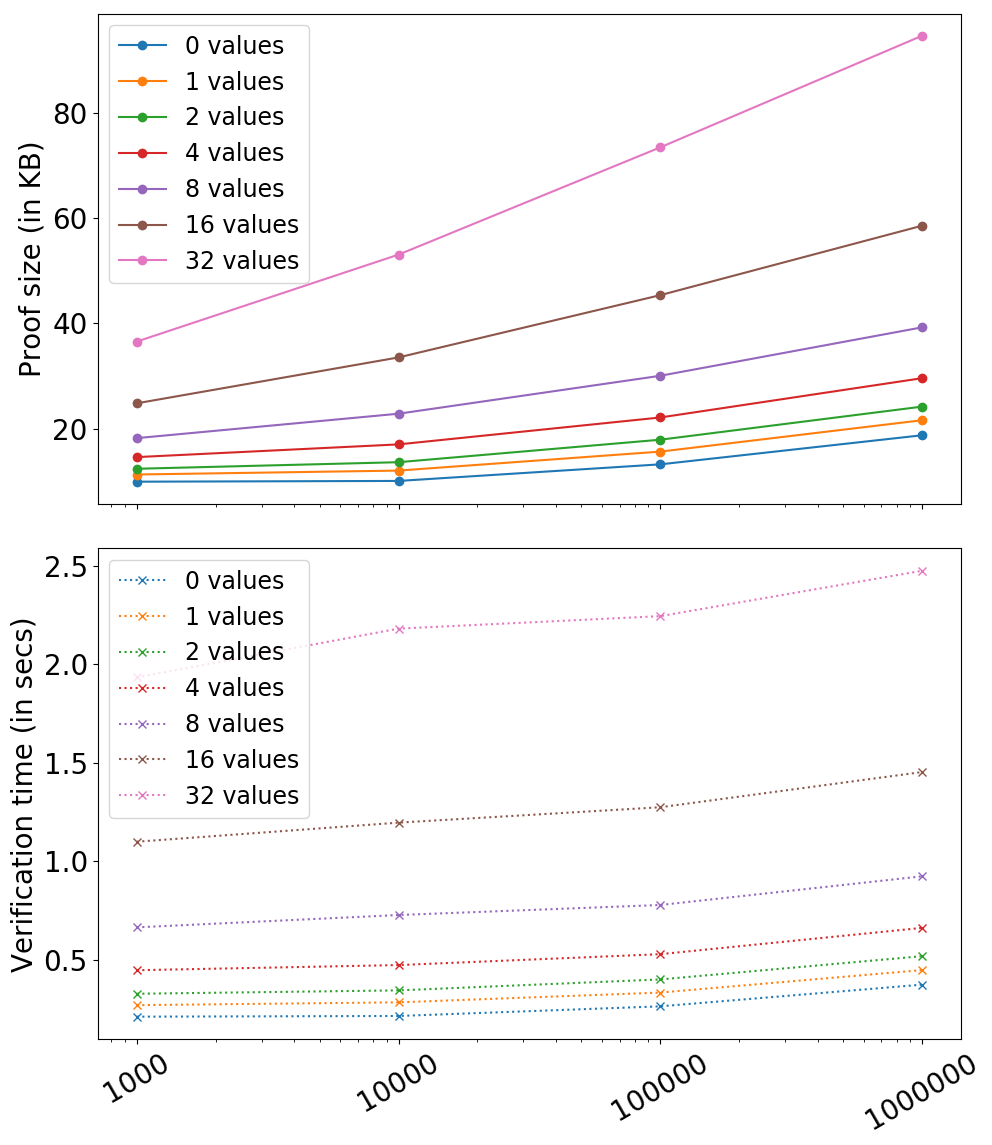
\includegraphics[width=0.32\linewidth]{figures/aad-memb-avg-case.png}
    \label{f:evaluation:lookup-avg}
}
\subfloat[Append times ($\uparrow$) and append-only proofs ($\downarrow$)]{\label{f:append-time}\label{f:append-only-proof}%
    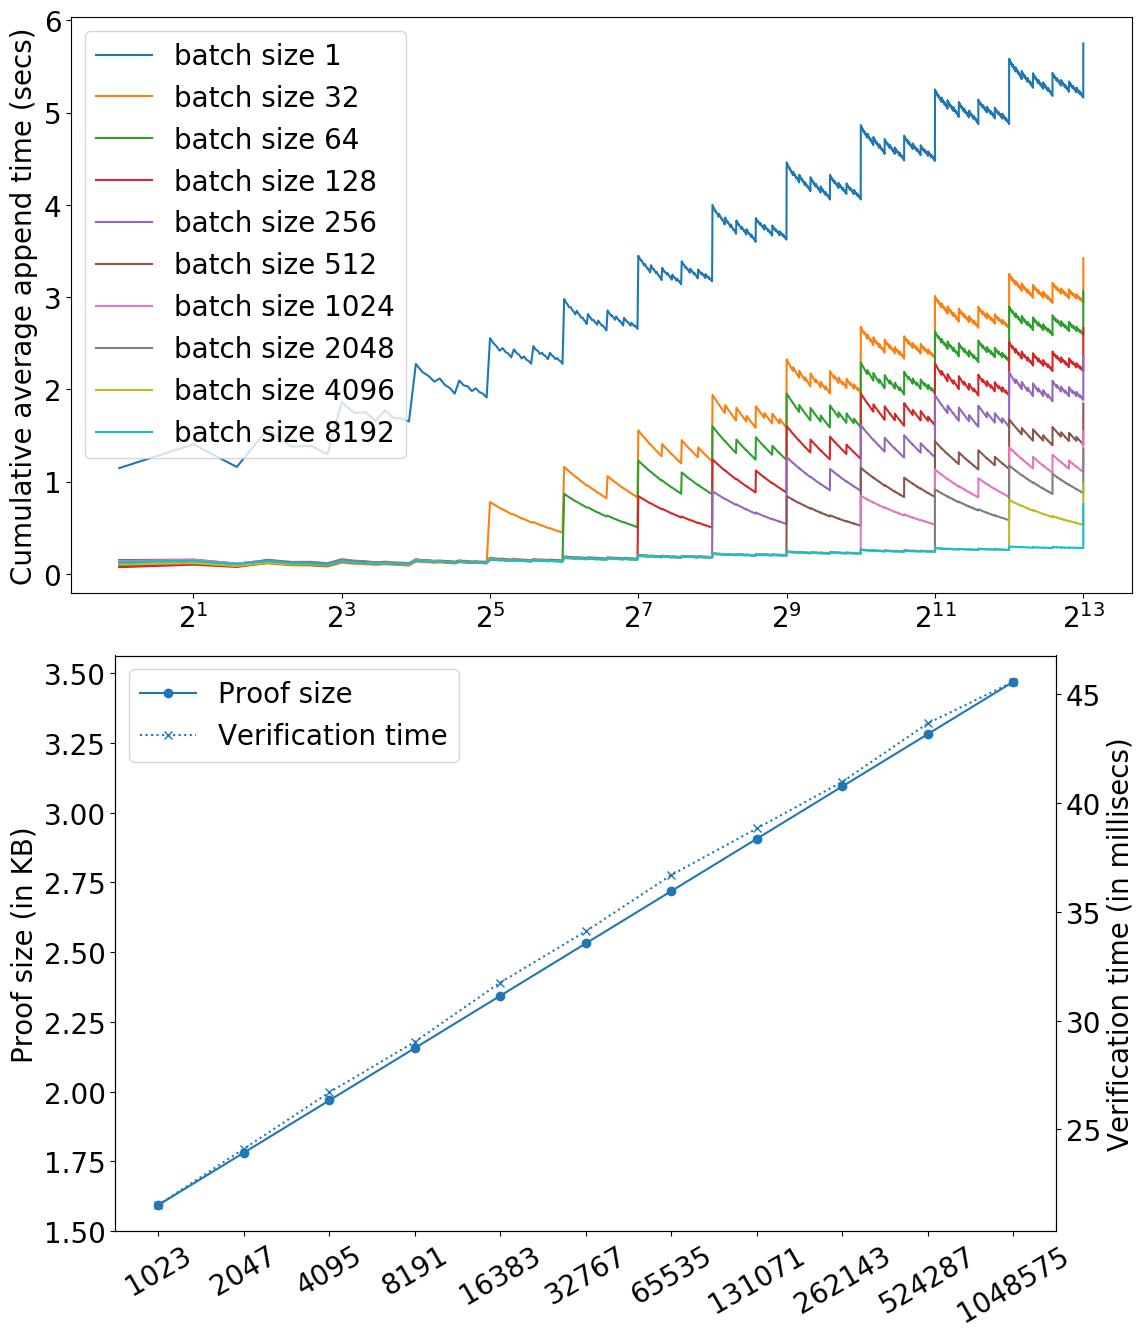
\includegraphics[width=0.32\linewidth]{figures/aad-merged-append-time-and-proof.png}
    \label{f:evaluation:append-time-and-proof}
}
\caption{
The x-axes always indicate AAD sizes.
\cref{s:eval:lookup,s:eval:append-only-proof,s:eval:append-time} explain the experiments.
In \cref{f:evaluation:append-time-and-proof} ($\uparrow$), ``spikes'' occur when two trees of size $B$ are merged, which triggers a new BFT computation, where $B$ is the batch size.
}
\label{f:evaluation}
\end{figure*}

\subsection{Microbenchmarks}

\subsubsection{Append times}
\label{s:eval:append-time}
% batch size 32
% 2019-02-04 10:50:34 36714 36714  PERF         benchAppends: 196 | Average time per append: 3422 milliseconds
% 
% batch size 64
% 2019-02-04 02:54:48 35509 35509  PERF         benchAppends: 196 | Average time per append: 3064 milliseconds
%
% batch size 128
% 2019-02-03 19:48:54 34590 34590  PERF         benchAppends: 196 | Average time per append: 2664 milliseconds
%
% batch size 256
% 2019-02-03 13:38:04 34156 34156  PERF         benchAppends: 196 | Average time per append: 2361 milliseconds
%
% batch size 512
% 2019-02-03 08:08:40 33620 33620  PERF         benchAppends: 196 | Average time per append: 1848 milliseconds
%
% batch size 1024
% 2019-02-03 03:13:40 30937 30937  PERF         benchAppends: 194 | Average time per append: 1548 milliseconds
%
% batch size 2048
% 2019-02-02 23:30:41 30167 30167  PERF         benchAppends: 194 | Average time per append: 1353 milliseconds
%
% batch size 4096
% 2019-02-02 20:15:01 29514 29514  PERF         benchAppends: 194 | Average time per append: 976 milliseconds
%
% batch size 8192
% 2019-02-02 17:47:11 28621 28621  PERF         benchAppends: 194 | Average time per append: 760 milliseconds
%

Starting with an empty AAD, we append key-value pairs to it and keep track of the \textit{cumulative average append-time}.
Recall that appends are amortized in our construction (but can be de-amortized using known techniques~\cite{overmars-van-leeuwen,overmars}).
As a result, in our benchmark some appends are very fast (e.g., 25 milliseconds) while others are painfully slow (e.g., 1.5 hours).
To keep the running time of our benchmark reasonable, we only benchmarked $2^{13} = 8192$ appends.
We also investigate the effect of batching on append times.
Batching $k = 2^i$ appends together means we only compute one BFT for the full tree of size $k$ created after inserting the batch.
In contrast, without batching, we would compute $k$ BFTs, one for each new forest root created after an append.
\cref{f:append-time} shows that the average append time is 5.75 seconds with no batching and 0.76 seconds with batch size 8192.
(For batch sizes $32, 64, \dots, 4096$, the average times per append in milliseconds are 3422, 3064, 2644, 2361, 1848, 1548, 1353 and 976 respectively.)
These times should increase by around 3.5 seconds if we benchmarked $2^{20}$ appends.

\parhead{Speeding up appends.}
The bottleneck for appends is computing the BFTs.
Although we used \texttt{libff}'s multi-threaded multi-exponentiation to compute accumulators faster, there are other ways to speed up appends that we have not explored.
First, we can parallelize computing (1) the polynomials on the same level in a BFT, (2) the smaller accumulators at lower levels of the BFT, where multi-threaded multi-exponentiation does not help as much and (3) the subset proofs in the forest.
Second, we can reuse some of the previously computed accumulators when computing a new BFT.
Third, our BPT and BFT constructions require ``extractable'' counterparts of the accumulators, which almost triple the time to commit to a polynomial.
We hope to remove this expensive requirement by proving our construction secure in the generic group model, similar to new SNARK constructions~\cite{groth16}.
Finally, techniques for distributed FFT could speed up polynomial operations~\cite{dizk}.

\subsubsection{Lookup proofs}
\label{s:eval:lookup}
We investigate three factors that affect lookup proof size and verification time: (1) the dictionary size, (2) the number of trees in the forest and (3) the number of values of a key.
Our benchmark creates AADs of ever-increasing size $n$.
For speed, instead of computing accumulators, we simply pick them uniformly at random.
(Note that this does not affect the proof verification time.)
We measure \textit{average} proof sizes for keys with $\ell$ values in an AAD of size $n$, where $\ell \in \{0, 1, 2, 4, 8, 16, 32\}$.
(Recall that a key with $\ell$ values requires $\ell$ frontier proofs.)
To get an average, for every $\ell$, we set up 10 different \textit{target} keys so each key has $\ell$ values.
The rest of the inserted keys are random (and simply ignored by the benchmark).
Importantly, we randomly disperse the target key-value pairs throughout the forest to avoid having all values of a key end up in consecutive forest leaves, which would artificially decrease the proof size.
Once the dictionary reaches size $n$, we go through every target key with $\ell$ values, compute its lookup proof, and measure the size and verification time.
% (Think of a lookup proof for $\ell = 0$ values as a non-membership proof.)
Then, for each $\ell$, we take an average over its 10 target keys.
We repeat the experiment for increasing dictionary sizes $n$ and summarize the numbers in \cref{f:lookup-avg,f:lookup-worst}.
Proof verification is single-threaded.

\parhead{Worst-case versus best-case dictionary sizes.}
Recall that some dictionary sizes are ``better'' than others because they have fewer trees in the forest.
For example, a dictionary of (worst-case) size $2^i - 1$ will have $i$ trees in the forest and thus $i$ BFTs.
Thus, a lookup proof must include frontier proofs in all $i$ BFTs.
In contrast, a dictionary of size $2^i$ only has a single tree in the forest, so a lookup proof needs only one {frontier proof}.
Indeed, our evaluation shows that lookup proofs are smaller in AADs of size $10^i$ (see \cref{f:lookup-avg}) compared to $2^i-1$ (see \cref{f:lookup-worst}).
For example, for a key with 32 values, the proof averages 95 KiB for size $10^6$ and 118 KiB for size $2^{20} - 1$.

%  aadSize  numValues  proofKiB    verifSecond
%  1000000          0   18.718750    0.372885
%  1000000          1   21.578125    0.446906
%  1000000          2   24.168750    0.517544
%  1000000          4   29.578125    0.661258
%  1000000          8   39.250000    0.923060
%  1000000         16   58.587500    1.452599
%  1000000         32   94.728125    2.474843

%  aadSize  numValues  proofKiB    verifSecond
%  1048575          0   41.934375    0.843512
%  1048575          1   44.803125    0.907273
%  1048575          2   47.390625    0.977507
%  1048575          4   52.418750    1.117400
%  1048575          8   62.350000    1.383276
%  1048575         16   81.684375    1.908019
%  1048575         32  118.112500    2.962104

\subsubsection{Append-only proofs}
\label{s:eval:append-only-proof}
This benchmark appends random key-value pairs until it reaches a target size $n = 2^{i+1} - 1$.
Then, it measures the append-only proof size (and verification time) between AADs of size $n$ and $m = 2^{i} - 1$.
We benchmarked on $2^{i}-1$ AAD sizes to illustrate worst-case $\Theta(i)$ append-only proof sizes.
To speed up the benchmark, we randomly pick accumulators in the forest.
Append-only proof verification is single-threaded.
Our results show append-only proofs are reasonably small and fast to verify (see \cref{f:append-only-proof}).
For example, the append-only proof between sizes $2^{19}-1$ and $2^{20}-1$ is 3.5 KiB and verifies in $45$ milliseconds.

\subsubsection{Memory usage.}
\label{s:eval:memory}
% Note: The 390x is from the FrontierSizeBench numbers in experiments/ccs19/frontier-size/20
\newcommand{\frontierOverhead}{390}
Our lookup proof benchmark was the most memory-hungry: it consumed 263 GiB of RAM for AAD size $n = 2^{20}-1$.
In contrast, the append-only proof benchmark consumed only 12.5 GiBs of memory, since it did not need BFTs.
As an example, when $n = 2^{20} - 1$, all BFTs combined have no more than $\frontierOverhead n$ nodes.
% This would normally require $2\cdot 32 + 64 = 128$ bytes per node, but \texttt{libff} needs 96 bytes per G1 and 192 per G2 => 384 for 2*G1 + G2
Since we are using Type~III pairings, each node stores three accumulators (two in $\Group_1$ and one in $\Group_2$) in 384 bytes (due to \texttt{libff}'s 3x overhead).
Thus, the BFT accumulators require no more than 147 GiB of RAM.
% 400 * (2^20-1) * (32*2 + 64) bytes in GiB        ----> 50 GiBs     (accs ideal)
% 400 * (2^20-1) * (96*2 + 192) bytes in GiB       ----> 150 GiBs    (accs w/ libff)
% 390 * (2^20-1) * (96*2 + 192) bytes in GiB       ----> 146.24 GiBs (accs w/ libff)
%
% Each node stores: left, right, parent and data pointer: 8*4 = 32 bytes
% 390 * (2^20-1) * (8*4) bytes in GiB              ----> 12.18 GiB   (root BFT pointer overhead)
% 450 * (2^20-1) * (8*3) bytes in GiB              ----> 10.54 GiB   (root BPT pointer overhead)
The rest of the overhead comes from our pointer-based BFT implementation and other bookkeeping (e.g., polynomials).
% $q$-PKE public parameters for an AAD of size $2^{20}$ take up at least 64 GiB of RAM: 512 * 2^20 * (32 bytes * 2 + 64 bytes), ignoring libff's 3x overhead.
The $q$-PKE public parameters could have added 64 GiBs of RAM, but these two benchmarks did not need them.

\parhead{Improving memory.}
A new security proof could eliminate the additional $\Group_1$ and $\Group_2$ accumulators and reduce BFT memory by 2.66x and the size of the public parameters by 1.33x (see \cref{s:eval:append-time}).
% i.e., in each pair of BFT siblings, we go from 2 * [ G_1, G_1, G_2 ] (32*2 + 64 bytes) to [ G_1 ] (32 bytes) in one node and [ G2 ] (64 bytes) in the sibling (so they can be paired)
% saves 2*(32+64) / (32 + 64) = 2.66x memory
% and eliminates g_1^{\tau s^i}'s, saving (32 * 2 + 64) / (32 + 64) = 1.33x memory
A more efficient representation of group elements than \texttt{libff}'s could also reduce BFT memory by 3x.
An efficient array-based implementation of BPTs and BFTs could further reduce memory by tens of gigabytes.
Finally, the 390x overhead of BFTs can be drastically reduced by carefully grouping upper frontier prefixes together in a BFT leaf, similar to the grouping of lower frontier prefixes from \cref{s:aad}.
However, doing this without increasing the lookup proof size too much remains to be investigated.
% The idea is that right now, each upper frontier prefix gets its own BFT leaf.
% This is because when proving non-membership of a key, we have to give a frontier proof for one of its missing prefixes.
% We do this by giving a subset path to a BFT leaf containing \textit{just} that missing prefix.
% But this means we incur a large computational overhead, creating roughly 2\lambda leaves for every newly inserted key's upper frontier prefixes.
% We could reduce this drastically by grouping upper frontier prefixes too (similar to how we group lower frontier prefixes).
% The downside is that, now, a frontier proof for an upper frontier prefix will be sending a path to a leaf with several other prefixes.
% To verify the leaf accumulator of this path, the verifier will have to recreate it from scratch.
% So he will need to be given the other/extra upper frontier prefixes in that leaf.
% This will slightly increase proof sizes, but could be mitigated against with compression.

\subsection{Comparison to Merkle tree approaches}
\label{s:eval:comparison-to-merkle}

How do AADs compare to Merkle prefix trees or History Trees (HTs), which are used in CONIKS and Certificate Transparency (CT) respectively?
First of all, appends in AADs are orders of magnitude slower because of the overheads of cryptographic accumulators and remain to be improved in future work (see \cref{s:eval:append-time}).

Lookup proofs in prefix trees are much smaller than in AADs.
% $\log_2(2^{20}) \cdot 32 = 640$ bytes
In a prefix tree of size $2^{20}$, a proof consisting of a Merkle path would be around $640$ bytes.
In comparison, our proofs for a key with 32 values are 152 times to 189 times more expensive (depending on the number of trees in the forest).
% 95 KiB / 640 bytes = 152x
% 118 KiB / 640 bytes = 189x
On the other hand, append-only proofs in AADs are $O(\log{n})$, much smaller than the $O(n)$ in prefix trees.
For example, our Golang implementation of prefix trees, shows that the append-only proof between trees of size $2^{19}$ and $2^{20}$ is 32 MiB (as opposed to 3.5 KiB in AADs).
The proof gets a bit smaller when the size gap between the dictionaries is larger but not by much: 14.6 MiB between $10^5$ and $10^6$.

Lookup proofs in history trees (HTs) are $O(n)$-sized, compared to $O(\log^2{n})$ in AADs.
This is because, to guarantee completeness, the HT proof must consist of all key-value pairs.
On the other hand, append-only proofs in AADs are slightly larger than in HTs.
While our proofs contain approximately the same number of nodes as in HT proofs, our nodes store two BPT accumulators in $\Group_1$ and a subset proof in $\Group_2$ (in addition to a Merkle hash).
This increases the per-node proof size from 32 bytes to 32 + 64 + 64 = 160 bytes.

% Sparse Merkle prefix tree proof sizes
% oldSize   newSize     appendOnlyProfSize
% 524,288   1,048,576   32 MiB
% 100,000   1,000,000   14.3 MiB

% Append-only proof sizes:
%  newDictSize  proofKiB  verifyMillisec
%         1023     1.59375      21.521
%         2047     1.78125      24.105
%         4095     1.96875      26.698
%         8191     2.15625      29.022
%        16383     2.34375      31.749
%        32767     2.53125      34.103
%        65535     2.71875      36.689
%       131071     2.90625      38.830
%       262143     3.09375      40.976
%       524287     3.28125      43.664
%      1048575     3.46875      45.573


\subsubsection{When do AADs reduce bandwidth?}
\label{s:eval:worth-it}
Asymptotically, AAD proof sizes outperform previous work.
But in practice, our evaluation shows AAD proof sizes are still larger than ideal, especially lookup proofs.
This begs the question: \textit{In what settings do AADs reduce bandwidth in transparency logs?}
We answer this question below while acknowledging that AAD append times and memory usage are not yet sufficiently fast for a practical deployment (see \cref{s:eval:append-time}).

\newcommand{\coniksfreq}{\ensuremath{\mathbf{\mathsf{D}}}\xspace}
\newcommand{\checkfreq}{\ensuremath{\mathbf{\mathsf{C}}}\xspace}

Consider a key transparency log with approximately one billion entries (i.e., an entry is a user ID and its PK).
If this were a CONIKS log, then each user must check their PK in every digest published by the log server.
Let \coniksfreq denote the number of digests published per day by the log server.
This means the CONIKS log server will, on average, send $960 \cdot \coniksfreq$ bytes per day per user (without accounting for the overhead of VRFs~\cite{vrf} in CONIKS).
If this were an AAD log, then each user (1) gets the most recent digest via an append-only proof and (2) checks their PK only in this digest via a lookup proof.
Let \checkfreq denote the number of times per day a user checks his PK (and note that, in CONIKS, $C = D$).
Since the lookup proof is for the user's PKs not having changed, it only needs to contain frontier proofs.
Extrapolating from \cref{f:lookup-avg}, such an average-case lookup proof is 40 KiB (in an AAD of size one billion).
Similarly, an append-only proof would be 7 KiB.
This means the AAD log server will, on average, send $47 \cdot 1024 \cdot C$ bytes per day per user.
Thus, AADs are more efficient when $.0199 \cdot D / C > 1$.
% Thus, if $C < (960 \cdot D) / (47\cdot 1024) =  0.0199 \cdot D$, then the AAD log server requires less bandwidth than CONIKS.
In other words, AADs will be more bandwidth-efficient in settings where log digests must be published frequently (i.e., $D$ is high) but users check their PK sporadically (i.e., $C$ is low).
% This should already be the case in key transparency, where all users should be able to register and update keys quickly (for availability reasons) even though some users might check their keys less often (since users can be offline).
For example, if $D=250$ (i.e., a new digest every 6 minutes) and $C=0.5$ (i.e., users check once every two days), then AADs result in 10x less bandwidth.

%% In CT, the server has to send   (certs_per_sec * cert_size_bytes * num_monitors)               bytes / sec
%% In AADs, the server has to send (47 * 1024 / (3600 * 24) * num_monitors * monitorings_per_day) bytes / sec
%%                                  .557 * num_monitors * monitorings_per_day)                    bytes / sec
%%
%% CT / AAD bandwidth overhead: 
%%      certs_per_sec * cert_size_bytes / (.557 * monitorings_per_day)
%%      17318 / (.557 monitorings_per_day)
%%      e.g., 1295.481 when monitoring once per hour (which is consistent with 483 GiBps / 383 MiBps)
%%
%% As long as:
%%      monitorings_per_day < certs_per_sec * cert_size_bytes / (47*1024/(3600*24))
%%      monitorings_per_day < certs_per_sec * cert_size_bytes / .557
%%      monitorings_per_day < 31,091.56
%% ...AADs result in less bandwidth.
What about CT?
Recall that CT lacks succinct lookup proofs.
As a result, domains usually trust one or more \textit{monitors} to download the log, index it and correctly answer lookup queries.
Alternatively, a domain can act as a monitor itself and keep up with every update to the log.
We call such domains \emph{monitoring domains}.
Currently, CT receives 12.37 certificates per second on average~\cite{ct-num-certs}, with a mean size of 1.4 KiB each~\cite{ct-avg-cert-size}.
Thus, a CT log server will, on average, send $12.37 \cdot 1.4 \cdot 1024 = 17,733.63$ bytes per second per monitoring domain.
In contrast, AADs require $47 \cdot 1024 \cdot C / 86,400 = .557\cdot C$ bytes per second per monitoring domain.
As before, $C$ denotes how many times per day a monitoring domain will check its PK in the log.
Thus, AADs are more efficient when $31,837 / C > 1$.
So even if domains monitor very frequently (e.g., $C = 100$), AADs are more bandwidth efficient.
However, we stress that our append times and memory usage must be reduced for a practical deployment to achieve these bandwidth savings (see \cref{s:eval:append-time,s:eval:memory}).

%% CONIKS bandwidth
%  ----------------
% Assume the CONIKS log publishes 10,000 digests per day.
% bytes_per_user = 960 bytes * 10,000 / day = 111.11 bytes/user/sec
% bytes_total = 111.11 bytes/user/sec * 1,000,000,000 = 103 GiBps
%
% If the frequency is to update the log once per hour, then CONIKS beats AADs.
% 960 bytes * 24 / day = 0.266666667 bytes/user/sec
% multiplied by 1,000,000,000 users, that's 254.31 MiBps.
% If it's once per minute, then the bandwidth would go to 253.31 MiBps * 60 = 14.9 GiBps.
% On the other hand, the proofs can be compressed using diffs, which could save a lot of traffic.

%% AAD bandwidth for CONIKS
%  ------------------------
% 47 KiB 10^9 / day = 47 KiB * 1024 bytes/KiB * 10^9 users / (24 hr/day * 60 min/hr * 60 sec/min) = 557037037 bytes/sec = 531.23 MiBps

%% CT bandwidth
%  ------------
% First CT log was launched in March 2013. Today is July 7, 2018 ([source](https://en.wikipedia.org/wiki/Certificate_Transparency#Certificate_authority_implementation))
% 1976 days between 03/01/2013 and 07/28/2018
% 2,112,278,786 certificates
% 1068966 certs/day
% 12.37 certs/second
% 1,400 bytes: the average size of a certificate
% 12.37 certs/sec * 1,400 bytes/cert = 17,318 bytes/sec
% 17,318 bytes/sec * 30 million = 519540000000 bytes/sec =  483 GiB/sec if 30 million domains monitor

%% AAD bandwidth for CT
%  --------------------
% 47 KiB * 1024 bytes/KiB * 30 million domains / hr = (47 * 1024 * 30*10^6 / 3600) / sec = 401,066,666.667 bytes/second = 383 MiBps

  % FIXED
\section{Discussion}
\label{s:discussion}
\label{s:aas:rsa}

\parhead{Privacy via VRFs.}
% Tree-based transparency logs like CONIKS provide some notion of privacy via the use of \textit{verifiable random functions (VRFs)}.
When a user's identity (e.g., email address) is hashed to determine a path in the tree, the existence of the path leaks that the user is registered.
To avoid this, CONIKS proposed using a \textit{verifiable random function (VRF)}~\cite{coniks,vrf} to map users to paths in the tree in a private but verifiable manner.
We note that our construction is compatible with VRFs as well and can provide the same guarantees.
For fairness, our comparison to CONIKS from \cref{s:eval:worth-it} assumes CONIKS does not use VRFs.

\parhead{Constant-sized digests.}
Digests in our constructions are $O(\log{n})$-sized where $n$ is the size of the set (or dictionary).
We can make the digest constant-sized by concatenating and hashing all Merkle roots.
Then, we can include the Merkle roots as part of our append-only and lookup proofs, without increasing our asymptotic costs.

\parhead{Large, bounded public parameters.}
Our bilinear-based constructions from~\cref{s:aas:construction,s:aad} are bounded: they support at most $N$ appends (given $q \approx 4\lambda N$ public parameters).
One way to get an unbounded construction might be to use RSA accumulators as explained later in this section.
Another way is to simply start a new data structure, when the old one gets ``full,'' similar to existing CT practices~\cite{Lynch2018}.
The old digest could be committed in the new data structure to preserve the append-only property and fork consistency.
(This will slightly increase our proof sizes for users who are not caught up with the latest digest.)
% This can be achieved by ``rotating'' our data structure.
% Assume the max size of the data structure is $2^{i+1} - 1$ (e.g., 1023 when $i=9$).
% We can provably discard the biggest tree of size $2^i$ (e.g., 512) but keep all other trees of sizes $2^{i-1}, 2^{i-2}, \dots, 1$ (e.g., $256, 128, \dots 1$).
% This creates room for another $2^i - 1$ appends (e.g., 511 appends).
% The remaining append is used to commit the discarded tree so as to preserve the append-only property.

\parhead{Trusted setup ceremony.}
Previous work shows how to securely generate public parameters for QAP-based SNARKs~\cite{groth10,groth16} via MPC protocols~\cite{zcash-mpc1,zcash-mpc2}.
For our AAD, we can leverage simplified versions of these protocols, since our public parameters are a ``subset'' of SNARK parameters.
In particular, the protocol from~\cite{zcash-mpc2} makes participation very easy: it allows any number of players to join, participate and optionally drop out of the protocol.
In contrast, the first protocol~\cite{zcash-mpc1} required a fixed, known-in-advance set of players.
For our scheme, we believe tech companies with a demonstrated interest in transparency logs such as Google, Facebook and Apple can be players in the protocol.
Furthermore, any other interested parties can be players too, thanks to protocols like~\cite{zcash-mpc2}.
Finally, the practicality of these MPC protocols has already been demonstrated.
In 2016, six participants used~\cite{zcash-mpc1} to generate public parameters for the Sprout version of the Zcash cryptocurrency~\cite{zcash}.
Two years later, nearly 200 participants used~\cite{zcash-mpc2} to generate new public parameters for the newer Sapling version of Zcash.

\parhead{RSA-based construction.}
% Requirements for AAS/AAD accumulators:
%  - Need subset proofs for append-only proofs in forest, for inclusion proofs and for frontier proofs. 
%  - Need disjointness for frontier. 
%  - Precomputing O(1) proofs like in RSA can also be helpful, both for the frontier and the forest.
In principle, the bilinear accumulator in our constructions from \cref{s:aas:construction,s:aad} could be replaced with other accumulators that support subset proofs and disjointness proofs.
Very recent work by Boneh et al.~\cite{batch-rsa-acc} introduces new techniques for aggregating non-membership proofs in RSA accumulators.
We believe their techniques can be used to create constant-sized disjointness proofs for RSA accumulators.
This, in turn, can be used to build an alternative AAD as follows.

Let us assume we have an RSA accumulator over $m$ elements.
First, RSA accumulators allow precomputing all \textit{constant-sized} membership proofs in $O(m\log{m})$ time~\cite{blind-auditable-memb-proofs}.
In contrast, our bilinear tree precomputes all logarithmic-sized proofs in $O(m\log^2{m})$ time.
As a result, frontier proofs would be constant-sized rather than logarithmic-sized (i.e., the frontier tree corresponding to an RSA accumulator would be ``flat'').
This decreases our AAD lookup proof size from $O(\log^2{n})$ to $O(\log{n})$.
This asymptotic improvement should also translate to a concrete improvement in proof sizes.
Our memory consumption should also decrease, since BFTs are no longer required.
Second, RSA accumulators have constant-sized parameters rather than linear in dictionary size.
This requires a simpler trusted setup ceremony~\cite{Frederiksen2018} and further saves memory on the server.
However, unless RSA accumulators can be sped up, it would result in even slower appends, due to more expensive exponentiations.
We leave it to future work to instantiate this RSA construction and prove it secure.

% Third, RSA accumulators do not require trusted setup if instantiated with class groups~\cite{batch-rsa-acc,Lipmaa2012} rather than the integers ${}\bmod N$.
% Although class groups are relatively new~\cite{Buchmann1988,Buchmann2001}, they have recently received increased interest~\cite{Damgaard2002,Pietrzak2018,Wesolowski2018,BonehBunzFisch2018,batch-rsa-acc,AltugChen2018}.

\subsection{Constructions from argument systems}
\label{s:snarks}%
% NOTE: https://youtu.be/jEHOZbKSHNI?t=547
%  - Aurora has O_k(N log N) prover time, O_k(log^2{N}) proof size and O_k(N) verification time, where k is a sec param
%
% NOTE: https://youtu.be/Y2HLlr3-MGA?t=1364
%  - Aurora and Ligero have O(n) verification time: 
%  - but STARK verifier complexity is wrong, since it should be polylog, I think (not linear)
%
% NOTE: Detailed table of complexities here: https://eprint.iacr.org/2019/099.pdf
%  - Bulletproofs is O(n log n) verifier
%  - says STARK verifier is polylog 
%  - hyrax complexity 
%
% NOTE: https://github.com/elibensasson/libSTARK also says STARK verifier is polylog

% d = depth of circuit
% n = circuit size
% Aurora:       transparent, PQ, \log^2{n} proof (220KB for n = 10^6), n\log{n} proving time, O(n) verification
% Ligero:       like aurora, except \sqrt{n} proof (4 MB)
% Hyrax:        like aurora, no PQ, except d\log{n} proof (50 KB)
% Bulletproofs: like aurora, no PQ, except \log{n} proof (1.5KB)
% STARK:        like aurora, except bigger constants for proof sizes (3.2 MB), verification time seems to be faster than SNARKs
% Kalai's new:  verification cost and proof size linear in the circuit depth, linear CRS, still requires trusted setup
%
% Micali's CS proofs: "Finally, Micali raises similar goals to ours in his work on computationally sound (CS) proofs [Mic94]. His results are however obtained in the random oracle model. This allows him to achieve CS-proofs for the correctness of general time computations with a nearly linear time verifier, a prover whose runtime is polynomial in the time complexity of the computation, and a poly-log length non-interactive (“written down” rather than interactive) proof." from GKR15 paper
%
% Summary: too large proofs, too large verification time, and unclear (concrete) prover complexity, since some of these use PCPs (e.g., STARKs).
%
A promising direction for future work is to build AADs from generic argument systems~\cite{groth10,groth16,qsp,cs-proofs,aurora,bulletproofs,ligero,hyrax,stark}.
Such AAD constructions would also require non-standard assumptions~\cite{GentryWichs2011}, possibly different than $q$-PKE (e.g., random oracle model, generic group model, etc.).
Depending on the argument system, they might or might not require trusted setup and large public parameters.

A static AAD can be built from an argument system (e.g., a SNARK~\cite{groth16,qsp}) as follows.
The AAD maintains one unsorted tree $U$ and one sorted tree $S$ whose leaves are sorted by key. 
The digest of the AAD consists of (1) the Merkle roots $(d(S), d(U))$ of $S$ and $U$ and (2) a SNARK \textit{proof of ``correspondence''} $\pi(S,U)$  between $S$ and $U$.
This proof shows that $S$'s leaves are the same as $U$'s \textit{but in a different, sorted by key, order}.
The SNARK circuit takes as input $U$'s leaves and $S$'s leaves, hashes them to obtain $d(U)$ and $d(S)$ and checks that $S$'s leaves are sorted by key.

Now, given a digest $(d(S), d(U), \pi(S,U))$, lookups can be efficiently proven using Merkle proofs in the sorted tree $S$.
The append-only property of two digests $(d(S), d(U), \pi(S,U))$ and $(d(S'), d(U')$, $\pi(S',U'))$ can be efficiently proven using a history tree append-only proof between $d(U)$ and $d(U')$. 
This proves $U$ is a subset of $U'$ and, crucially, it also proves that $S$ is a subset of $S'$, since the SNARK $\pi(S,U)$ proves that $S$ ``corresponds'' to $U$ and $S'$ to $U'$.
Unfortunately, updates would invalidate the SNARK proof and take time at least linear in the dictionary size to recompute it.
However, we can apply the same Overmars technique~\cite{overmars,overmars-van-leeuwen} to make updates polylogarithmic time.
(This would now require a family of circuits, one for each size $2^i$ of the trees.)

This approach would result in much shorter lookup proofs while maintaining the same efficiency for append-only proofs, since state-of-the-art SNARKs have proofs consisting of just 3 group elements~\cite{groth16}.
% $O(\log^2{n})$ lookup proofs, $O(\log{n})$ append-only proofs, $O(n)$ storage and, we estimate, $O(\log^3{n})$ append time if instantiated with state-of-the art SNARKs~\cite{groth16}.
On the other hand, this approach might need more public parameters and could have slower appends.
This is because, even with SNARK-friendly hashes (e.g., Ajtai-based~\cite{cycles-of-ec}, MiMC~\cite{mimc} or Jubjub~\cite{jubjub}), we estimate the number of multiplication gates for hashing trees of size $2^{20}$ to be in the billions.
(And we are not accounting for the gates that verify tree $S$ is sorted.)
In contrast, the degrees of the polynomials in our bilinear-based constructions are only in the hundreds of millions for dictionaries of size $2^{20}$.

Nonetheless, optimizing such a solution would be interesting future work.
For example, replacing SNARKs with STARKs~\cite{stark} would eliminate the large public parameters and the trusted setup, at the cost of larger append-only proofs.
This may well be worth it if the proof size and prover time are not too large.
Other argument systems such as Hyrax~\cite{hyrax}, Ligero~\cite{ligero} and Aurora~\cite{aurora} could achieve the same result.
Unfortunately, Aurora and Ligero would increase the append-only proof verification time to linear, which could be prohibitive.
Bulletproofs~\cite{bulletproofs} would further increase this verification time to quasilinear.
Hyrax can make this time sublinear if the circuit is sufficiently parallel or has ``a wiring pattern [that] satisfies a technical regularity condition''~\cite{hyrax}.

\parhead{Recursively-composable arguments.}
Another interesting approach is to obtain AADs from recursively-composable SNARKs~\cite{cycles-of-ec,BitanskyCanettiChiesaTromer2013}.
Such SNARKs could structure the verification of the append-only property recursively so that circuits need not operate on the entire dictionary, thus lowering overheads.
We are aware of concurrent work that explores this approach, but unfortunately it is not peer-reviewed nor published in an online archive.
While such an approach could be very promising, currently implemented systems operate at the 80-bit security level.
This is because increasing the security of the elliptic curves used in recursive SNARK constructions is costly, since they have low embedding degree~\cite{cycles-of-ec}.
% For BN254: \sqrt{p/q} = \sqrt{2^220/2^20} = 2^100
In contrast, our implementation is 100-bit-secure after accounting for recent progress on computing discrete logs~\cite{MenezesSarkarSingh2017} and our $q$-SDH assumption with $q=2^{20}$~\cite{BonehBoyen2008}.
% For BLS12-318: \sqrt{p/q} = \sqrt{2^256/2^20} = \sqrt{2^236} = 2^118
We can increase this to 118 bits, with no loss in performance, by adopting 128-bit-secure BLS12-381 curves~\cite{bls12-381-switch}.

  % FIXED
\section{Conclusion}
In this work, we introduced the first append-only authenticated dictionary (AAD) that achieves polylogarithmic proof sizes and append times.
Unlike previous work, our construction only assumes a single fully-malicious server and does not rely on users to ``collectively'' verify the dictionary.
Our analysis shows that AADs can reduce the bandwidth in current CT logs and in CONIKS logs that publish digests much more frequently than users check their PK in the log.
However, as our evaluation shows, AADs are not yet practical enough for deployment, particularly because they have high append times and memory usage.
We hope future work can overcome this by optimizing the construction, the implementation or both.
Finally, we also introduced the first efficient append-only authenticated set (AAS), which can be used to implement Google's Revocation Transparency (RT)~\cite{rev-transparency}.

\parhead{Open problems.}
We identify two interesting directions for future work.
First, can we build efficient AADs with polylogarithmic proof sizes from standard assumptions, such as the existence of CRHFs?
If not, what are the lower bounds?
Second, can we obtain ``zero-knowledge'' AADs which leak nothing during queries?

  % FIXED
\section*{Acknowledgments}
\label{sec:acknowledgments}
We would like to thank Marten van Dijk for suggesting the ``sparse'' prefix tree approach and Madars Virza for productive conversations that helped steer this work.
We also thank the anonymous reviewers for their useful feedback.
This research was supported in part from USA NSF under CNS grants 1413920, 1718782, 1514261, 1652259, by DARPA \& SPAWAR under grant N66001-15-C-4066, by HK RGC under grant ECS-26208318, and by a NIST grant.

  %\clearpage
  \balance
  \bibliographystyle{ACM-Reference-Format}
  \bibliography{references}
  \balance

  %\clearpage
  \appendix
  % FIXED
\section{Cryptographic Assumptions}
\label{app:assumptions}

\begin{definition}[Bilinear pairing parameters]
    \label{d:bilinear-pairing-parameters}
    Let $\mathcal{G}(\cdot)$ be a randomized polynomial algorithm with input a security parameter $\lambda$.
    % -- begin multiline --
    Then, $\langle \Group, \GT, p, g, e\rangle \leftarrow \mathcal{G}(1^\lambda)$ are called bilinear pairing parameters if
    $\Group$ and $\GT$ are cyclic groups of prime order $p$ where discrete log is hard, 
    $\Group = \langle g \rangle$ (i.e., $\Group$ has generator $g$)
    and if $e$ is a bilinear map, $e : \Group\times \Group \rightarrow \GT$ such that $\GT = \langle e(g,g) \rangle$.
    % -- end multiline --
    %For $\lambda$ bits of security on computing discrete logs in $\Group$ and $\GT$, we require that $p > 2^{2\lambda}$.
\end{definition}

Our security analysis utilizes the following two cryptographic assumptions over elliptic curve groups with bilinear pairings.
\begin{definition}[$q$-SBDH Assumption]
\label{d:q-sbdh}
Given security parameter $\lambda$, bilinear pairing parameters $\langle \Group, \GT, p, g, e\rangle \leftarrow \mathcal{G}(1^\lambda)$,
public parameters  $\langle g, g^s, g^{s^2},\allowbreak \dots, g^{s^q}\rangle$ for some $q = \poly(\lambda)$ and some $s$ chosen uniformly at random from $\Zp^*$, no probabilistic polynomial-time adversary can output a pair $\langle c, e(g,g)^\frac{1}{s+c}\rangle$ for some $c \in \Zp$, except with probability negligible in $\lambda$.
\end{definition}

% Note: Adversary is given g^{s^i} and g^{\tau s^i} but not given \tau and outputs (c', c) s.t. c' = c^\tau. 
% The assumption says that the only way the adversary can output such a tuple, is by setting c = {g^{s^i}}^a_i and c' = {g^{\tau s^i}}^a_i for *known* a_i's. In other words, if c \ne g^{a_i s^i}.
\begin{definition}[$q$-PKE Assumption]
\label{d:q-pke}
The $q$-power knowledge of exponent assumption holds for $\mathcal{G}$ if for all probabilistic polynomial-time adversaries $A$, there exists a probabilistic polynomial time extractor $\chi_A$ such that for all \emph{benign} auxiliary inputs $z \in \{0,1\}^{\poly(\lambda)}$ 
\begin{align*}
\Pr \left[ \begin{array}{c}
    \langle \Group, \GT, p, g, e\rangle \leftarrow \mathcal{G}(1^\lambda); \langle s, \tau\rangle \leftarrow \Zp^*;\\
    \sigma \leftarrow \langle \Group, \GT, p, g, e, \mathcal{PP}_q(s, \tau)\rangle;\\
    \langle c, \hat{c}; a_0, a_1, \dots, a_q\rangle \leftarrow (A||\chi_A)(\sigma,z):\\
    \hat{c} = c^\tau \wedge c \ne g^{\prod_{i=0}^q {a_i s^i}}
\end{array} \right] = \mathsf{negl}(\lambda)
\end{align*}
where $\langle y_1; y_2\rangle \leftarrow (A||\chi_A)(x)$ means $A$ returns $y_1$ on input $x$ and $\chi_A$ returns $y_2$ given the same input $x$ and $A$'s random tape.
Auxiliary input $z$ is required to be drawn from a benign distribution to avoid known negative results associated with knowledge-type assumptions~\cite{neg1,neg2}.
\end{definition}
  % FIXED
\section{AAS Algorithms}
\label{s:aas:algorithms}
Here, we give detailed algorithms that implement our AAS from \cref{s:aas}.
Recall that our AAS is just a forest of BPTs with corresponding BFTs.
In particular, observe that each forest node has a BPT accumulator associated with it, while root nodes in the forest have BFTs associated with them.
Our algorithms described below operate on this forest, adding new leaves, merging nodes in the forest and computing BFTs in the roots.

\parhead{Trees notation.}
\label{s:prelim:notation:trees}
The $|$ symbol denotes string concatenation.
A \textit{tree} is a set of nodes denoted by binary strings in a canonical way.
The root of a tree is denoted by the empty string $\varepsilon$ and the left and right children of a node $w$ are denoted by $w|0$ and $w|1$ respectively.
If $b\in\{0,1\}$, then the sibling of $w = v|b$ is denoted by $\sibling(w) = v|\overline{b}$, where $\overline{b} = 1-b$.
A \emph{path} from one node $v$ to its ancestor node $w$ is denoted by $\treepath[v,w] = \{u_1 = v, u_2 = \parent(u_1), \dots, u_\ell = \parent(u_{\ell-1}) = w\}$.
The parent node of $v = w|b$ is denoted by $\parent(v) = \parent(w|b) = w$.
We also use $\treepath[v,w) = \treepath[v,w]-\{w\}$.

\parhead{Forest notation.}
\label{s:prelim:notation:forests}
Let $F_i$ denote a forest of up to $\beta$ leaves that only has $i$ leaves in it (e.g., see \cref{f:forest}).
Intuitively, a forest is a set of trees where each tree's size is a \textit{unique} power of two (e.g., see $F_5$ in \cref{f:forest}).
The unique tree sizes are maintained by constantly merging trees of the same size.
% When \beta = 1, there will be one leaf with 0 bits (\ceil(\log(1)) = 0): the empty string.
% When \beta = 2, we need \ceil(\log(2)) = 1 bit for each of the two leaves, and their root will be the empty string, and so on.
% When \beta = 3, we need \ceil(\log(3)) = 2 bits for each of the three leaves.
Let $\bin^\beta(x)$ denote the $\ceil{\log{\beta}}$-bit binary expansion of a number $x$ (e.g., $\bin^{14}(6)=0110$).
(Note that $\bin^1(x) = \varepsilon,\forall x$ because $\ceil{\log{1}}=0$.)
In our AAS, $\bin^\beta(i)$ denotes the $i$th inserted leaf, where $i$ starts at 0 (e.g., see leaves 000 through 111 in $F_5$ in \cref{f:forest}).
Let $\roots(F_i)$ denote all the roots of all the trees in the forest (e.g., $\roots(F_5) = \{0, 111\}$ in \cref{f:forest}).
Let $\leaves(F_i)$ denote all the leaves in the forest (e.g., $\leaves(F_3) = \{000, 001, 010\}$ in \cref{f:forest}).

\parhead{AAS notation.}
Note that \textbf{assert$(\cdot)$} ensures a condition is true or fails the calling function otherwise. 
Let $\dom(f)$ be the domain of a function $f$. %(i.e. $\forall x \in \dom(f), \exists y$ such that $f(x) = y$).
We use $f(x)=\bot$ to indicate $x\notin \dom(f)$.
Let $\AS_i$ denote our AAS with $i$ elements.
Each node $w$ in the forest stores extractable accumulators $\acc_w, \eacc_w$ of its BPT together with a Merkle hash $\hash_w$.
Internal nodes (i.e., non-roots) store a subset proof $\subsetProof_w$ between $\acc_w$ and $\acc_{\parent(w)}$.
The digest $d_i$ of $\AS_i$ maps each root $r$ to its Merkle hash $\hash_r$.
Every root $r$ stores a disjointness proof $\disj_r$ between its BPT and BFT.
For simplicity, we assume server algorithms implicitly parse out the \myblue{\textbf{bolded blue variables}} from $\AS_i$.
% The algorithms below sometimes incrementally build a function $f$ by adding new points $\left(u, v = f(u)\right)$ to its graph, either via $f = f\cup \{(u,v)\}$ or via $f(u) \gets v$.

\parhead{Server algorithms.}
{\setup}$(\cdot)$ generates large enough $q$-PKE public parameters $\mathcal{PP}_q(s,\tau)$ (see \cref{d:q-pke}), given an upper bound $\beta$ on the number of elements.
Importantly, the server forgets the trapdoors $s$ and $\tau$ used to generate the public parameters.
In other words, this is a \emph{trusted setup} phase (see \cref{s:discussion}).

% Assuming elements are hashed to 2\lambda bits:
%
% The size of the AAS server public parameters
% --------------------------------------------
% \beta > 0 is the max # of elements
% When \beta = 2^k:
%  - the worst-case forest has a single BPT with \beta leaves, one for each element
%  - each element has 2\lambda bits and thus 2\lambda + 1 prefixes (b.c. we include the empty prefix \varepsilon, which we could exclude actually, since all elements have it)
%  - so, the root node of the BPT accumulates (2\lambda + 1)\beta prefixes (this is only true for \beta = 1 because, when \beta > 1, some prefixes will coincide)
% When 2^k < \beta < 2^{k+1}:
%  - the worst-case forest's largest BPT has \ell = 2^{\floor{\log{\beta}}} leaves
%    (e.g., If \beta = 10, the largest BPT will have 8 leaves, and the next BPT will have 2 leaves.
%     Incidentally, when \beta is not a power of two, we actually support adding more than \beta elements: 2^{k+1} - 1 to be exact.
%     For \beta = 10, we can add 8 + 4 + 2 + 1 = 15.)
%  - so, the root node of the BPT accumulates (2\lambda+1)\ell prefixes
%
% So, in general, we need (2\lambda+1)\ell prefixes in the root node of the largest BPT, where \ell = 2^{\floor{\log{\beta}}}
% Since a polynomial $\sum_{i=1}^q (x-r_i)$ with $q$ roots has degree $q$, that means the degree of the root BPT accumulator will be (2\lambda+1)\ell.
% (Note: In the implementation, we could avoid accumulating the empty prefix, since all keys will have it. But we do not.)
%
% The size of the AAS clients public parameters
% ---------------------------------------------
% The client needs to be able to reconstruct any leaf accumulato over 2\lambda+1 prefixes.
% So he needs to commit to polynomials of degree exactly $q=2\lambda + 1$

\begin{algorithm}[H]
    \footnotesize
    \begin{algorithmic}[1]
    \caption{\small Computes public parameters (trusted setup)}
    \label{a:aas:setup}
    \Function{\setup}{$1^\lambda, \beta$} $\rightarrow (pp, VK)$ \Comment{Generates $q$-PKE public parameters}
        \State
            $\ell \gets 2^{\floor{\log{\beta}}} \qquad
             q \gets (2\lambda + 1)\ell \qquad
             ( \Group,\GT,p,g,e(\cdot,\cdot) ) \leftarrow \mathcal{G}(1^\lambda)$
        \State
            $s\stackrel{\$}{\gets} \Fp \qquad
             \tau\stackrel{\$}{\gets} \Fp \qquad
             VK=((g^{s^i})_{i=0}^{2\lambda + 1}, g^\tau)$
        \State \Return $((( \Group,\GT,p,g,e(\cdot,\cdot) ), \beta, \mathcal{PP}_q(s,\tau)), VK )$
    \EndFunction
    \end{algorithmic}
\end{algorithm}

{\append}$(\cdot)$ creates a new leaf $\ell$ for the element $k$ (\crefrange{a:aas:append:create-leaf-begin}{a:aas:append:create-leaf-end}).
Recursively merges equal-sized BPTs in the forest, as described in \cref{s:aas:construction} (\crefrange{a:aas:append:merge-begin}{a:aas:append:merge-end}).
In this process, computes subset proofs between old BPT roots and the new BPT.
Merging ends when the newly created BPT $w$ has no equal-sized BPT to be merged with.
Recall from \cref{s:prelim:polycommit} that $\Hp$ maps elements to be accumulated to field elements in $\Fp$.
\begin{algorithm}[H]%[tb] % sigle column
    \caption{\small Appends a new $i$th element to the AAS, $i\in[0,\beta-1]$}
    \label{a:aas:append}
    \footnotesize
    \begin{algorithmic}[1]
    \Function{\append}{$pp,\AS_i, d_i, k$} $\rightarrow (\AS_{i+1}, d_{i+1})$
        \State $w \gets \bin^\beta(i) \qquad \elems_w \gets \{k\}$\Comment{Create new leaf $w$ for element $k$}
        \label{a:aas:append:create-leaf-begin}
        \State $(\accpoly_w, {\acc}_w, \cdot) \gets \accumulate(P(\elems_w)) \quad \hash_w \gets \Hb(w|\bot|{\acc}_w|\bot)$
        \label{a:aas:append:create-leaf-end}

        \LineComment{``Merge'' old BPT roots with new BPT root (recursively)}
        \While{$\sibling(w)\in \roots(F_i)$}
        \label{a:aas:append:merge-begin}
            \State $\ell \gets\sibling(w) \qquad p\gets \parent(w) \qquad \elems_p \gets \elems_\ell\cup \elems_w$
            \State $(\accpoly_p, {\acc}_p, \eacc_p) \gets \accumulate(P(\elems_p))\qquad \hash_p = \Hb(p|\hash_\ell|{\acc}_p|\hash_w)$
            \State $(\cdot, \subsetProof_\ell, \cdot) \gets \accumulate(P(\elems_p\setminus \elems_\ell))$
            \State $(\cdot, \subsetProof_w, \cdot) \gets \accumulate(P(\elems_p \setminus \elems_w)) \qquad w\gets p$
        \EndWhile
        \label{a:aas:append:merge-end}
        % Note: Adding a single leaf will always create exactly one new root, possibly by merging more than two old roots.

        \LineComment{Invariant: $w$ is a new root in $F_{i+1}$. Next, computes $w$'s frontier.}
        \label{a:aas:append:root-at-begin}
        \State $(\fropoly_w,\bft_w) \gets \createfrontier(F(\elems_w))$
        % We need frontier polynomial \fropoly_w here to compute the EEA coeffs below!
        \State $(y,z)\gets \mathsf{ExtEuclideanAlg}(\accpoly_w, \fropoly_w)\qquad {\disj}_w \gets ( g^{y(s)}, g^{z(s)})$
        \label{a:aas:append:root-at-end}

        \State Store updated AAS state (i.e., the \myblue{\textbf{bolded blue}} variables) into $\AS_{i+1}$
        \State $d_{i+1}(r) \gets \hash_r, \forall r \in \roots(F_{i+1})$\Comment{Set new digest}
        \State \Return $\AS_{i+1}, d_{i+1}$
    \EndFunction

    % Note that this function is implicitly given access to all the public parameters it needs.
    \Function{\accumulate}{$T$}
        \State \Return $(\accpoly, g^{\accpoly(s)}, g^{\tau \accpoly(s)})$ where $\accpoly(x)=\prod_{w \in T} {(x-\Hp(w))}$
    \EndFunction
    \end{algorithmic}
\end{algorithm}

If $k$ is in the set, $\provememb(\cdot)$ sends a Merkle path to $k$'s leaf in some tree with root $r$ (\crefrange{a:aas:provememb:paths-begin}{a:aas:provememb:paths-end}) via $\provepath(\cdot)$ (see \cref{a:aas:provepath}).
This path contains subset proofs between every node's accumulator and its parent node's accumulator.
If $k$ is not in the set, then $\provememb(\cdot)$ sends frontier proofs in each BFT in the forest (\crefrange{a:aas:provememb:frontier-begin}{a:aas:provememb:frontier-end}) via $\provefrontier(\cdot)$ (see \cref{a:at:provefrontier}).

\begin{algorithm}[H]%[tb] % sigle column
    \caption{\small Constructs a (non)membership proof}
    \label{a:aas:provememb}
    \label{a:aas:provepath}
    \footnotesize
    \begin{algorithmic}[1]
    \Function{\provememb}{$pp,\AS_i,k$} $\rightarrow (b,\pi)$
        \State Let $\ell\in \leaves(F_i)$ be the leaf where $k$ is stored or $\bot$ if $k\notin \AS_i$
        \If{$k \in \AS_i$} \Comment{Construct Merkle path to element}
            \label{a:aas:provememb:paths-begin}
            \State Let $r\in \roots(F_i)$ be the root of the tree where $k$ is stored
            \State $\pi \gets \provepath(\AS_i, \ell, r,\bot)\qquad b\gets 1$ % \qquad R\gets R-\{r\}
            \label{a:aas:provememb:paths-end}
        \Else \Comment{Prove non-membership in all BFTs}
            \label{a:aas:provememb:frontier-begin}
            \State $\CP_r\gets \provefrontier(\AS_i,r,k),\forall r\in \roots(F_i)$
            % We don't need extractability for BPT accumulators in non-membership proofs
            % We do need the hashes of the root's children (if any) for the client to verify this BPT accumulator against the Merke root hash
            % (note if r|c does not exist because r is a leaf, then we assume h_{r|c} equals \bot)
            \State $\pi\gets \proverootaccs(\AS_i, \pi)\quad b\gets 0$
            \label{a:aas:provememb:frontier-end}
        \EndIf
        \State \Return $b, ( \ell, \pi, (\CP_r)_{r\in \roots(F_i)}, (\disj_r)_{r\in \roots(F_i)})$
    \EndFunction

    % Includes leaf (u) and root (r) BPT accumulators, as well as (u)'s subset proof
    \Function{\provepath}{$\AS_i,u,r,\pi$} $\rightarrow \pi$\Comment{Precondition: $r$ is a root in $F_i$}
        \State $\pi(r) \gets ( \bot, \acc_r, \eacc_r, \bot)$
        \LineComment{Overwrites $\pi(w)$ set by previous \provepath call (if any)}
        \State $\pi(w) \gets ( \bot, \acc_w, \eacc_w, \subsetProof_w), \forall w\in \treepath[u,r)$
        \LineComment{Only sets $\pi(\sibling(w))$ if not already set from previous \provepath call!}
        \For{$w\in \treepath[u,r)$ where $\sibling(w)\notin \dom(\pi)$}
            \State $\pi(\sibling(w)) \gets ( \hash_{\sibling(w)}, \bot,\bot,\bot)$
        \EndFor
        \State \Return $\pi$
    \EndFunction

    \Function{\proverootaccs}{$\AS_i,\pi$} $\rightarrow \pi$
        % Note: Non-membership proofs don't need the extractable counterpart, but \verappendonly does.
        \State $\pi(r)\gets (\bot,\acc_{r}, \eacc_{r}, \bot), \forall r\in\roots(F_i),$
        \State $\pi(r|c)\gets (\hash_{r|c},\bot,\bot,\bot), \forall r\in\roots(F_i), \forall c\in \{0,1\}$
    \EndFunction
    \end{algorithmic}
\end{algorithm}

For each root $r$ in $F_i$, {\proveappendonly}$(\cdot)$ sends a Merkle path to an ancestor root in $F_j$, if any.
The Merkle path contains subset proofs between all BPT accumulators along the path.
It also contains the root BPT accumulators from $F_i$, which the client will verify against his digest $d_i$.

\parhead{Client algorithms.}
{\verappendonly}$(\cdot)$ first ensures that $d_i$ and $d_j$ are digests at version $i$ and $j$ respectively (\crefrange{a:aas:verappendonly:check-digest-begin}{a:aas:verappendonly:check-digest-end}).
Before checking subset proofs, {\verappendonly}$(\cdot)$ validates the old root BPT accumulators in $\pi_{i,j}$ against the Merkle roots in $d_i$ (\crefrange{a:aas:verappendonly:check-old-root-accs-begin}{a:aas:verappendonly:check-old-root-accs-end}).
Then, checks that each root $r$ from $F_i$ is a subset of some root in $F_j$ by checking subset proofs (\cref{a:aas:verappendonly:paths}) via $\verpath(\cdot)$ (see \cref{a:helper:verpath}).
{\verappendonly}$(\cdot)$ enforces fork-consistency implicitly when verifying Merkle hashes.

\begin{algorithm}[H]%[tb] % sigle column
    \caption{\small Creates and verifies append-only proofs}
    \label{a:aas:proveappendonly}
    \label{a:aas:verappendonly}
    \footnotesize
    \begin{algorithmic}[1]
    \Function{\proveappendonly}{$pp,\AS_i,\AS_j$} $\rightarrow \pi$
        \If{$\roots(F_i)\subset\roots(F_j)$}
            \Return $\bot$
        \EndIf
        \State Let $R=\{$roots $\in F_i$ but $\not\in F_j\}$ and $r'\in \roots(F_j)$ be their ancestor root
        % Note: When adding two paths, appends to proof \pi or even overwrites it
        \State $\pi\gets \provepath(\AS_j, r,r',\pi), \forall r \in R\quad \pi\gets\proverootaccs(\AS_i,\pi)$
        \State \Return $\pi$
    \EndFunction

    \Function{\verappendonly}{$VK, d_i, i, d_j, j, \pi_{i,j}$} $\rightarrow \{T,F\}$
        % Version of digest is implicitly given by the node numbering fixed through Merkle hashing
        % For the fork-consistency definition, VerAppendOnly needs to check the old version of the digest too (technicality).
        \Assert $d_i(r) \ne \bot \Leftrightarrow r\in \roots(F_i)$ \Comment{Is valid version $i$ digest?}
        \label{a:aas:verappendonly:check-digest-begin}
        \Assert $d_j(r) \ne \bot \Leftrightarrow r\in \roots(F_j)$ \Comment{Is valid version $j$ digest?}
        \label{a:aas:verappendonly:check-digest-end}
        \Assert $\forall r \in \roots(F_i) \cap \roots(F_j), d_i(r)=d_j(r)$
        
        \State Let $R=\{$roots $\in F_i$ but $\not\in F_j\}$ \Comment{i.e., old roots with paths to new root}
        % Recall that d_i(r) only stores the Merkle root hash h_r and not the BPT accumulator a_r.
        % The proof \pi_{i,j} will give a_r but it could give a completely different one, breaking the append-only property.
        % Thus, whatever it gives must be verified.
        \ForAll{$r\in \roots(F_i)$} \Comment{Check proof gives correct old root accumulators}
            \label{a:aas:verappendonly:check-old-root-accs-begin}
            \State $(\cdot,a_{r},\cdot,\cdot)\gets \pi(r)$ \quad $({h}_{r|b},\cdot,\cdot,\cdot) \gets \pi(r|b),\forall b\in \{0,1\}$
            \Assert $d_i(r) = \Hb(r|h_{r|0}|a_r|h_{r|1})$
        \EndFor
        \label{a:aas:verappendonly:check-old-root-accs-end}
        \State $\forall r\in R$, fetch $h_r$ from $d_i(r)$ and update $\pi_{i,j}(r)$ with it
        \Assert $\pi_{i,j}$ is well-formed Merkle proof for all roots in $R$
        \Assert $\forall r\in R,\verpath(d_j, r, \pi_{i,j})$
        \label{a:aas:verappendonly:paths}
    \EndFunction
    \end{algorithmic}
\end{algorithm}

If $k$ is stored at leaf $\ell$ in the AAS, {\vermemb}$(\cdot)$ reconstructs $\ell$'s accumulator from $k$.
Then, checks if there's a valid Merkle path from $\ell$ to some root, verifying subset proofs along the path via $\verpath(\cdot)$ (see \cref{a:helper:verpath}).
If $k$ is not in the AAS, {\vermemb}$(\cdot)$ verifies frontier proofs for $k$ in each BFT in the forest via $\verfrontier(\cdot)$ (see \cref{a:at:verfrontier}).

\begin{algorithm}[H]%[tb] % single column
    \caption{\small Verifies a (non)membership proof}
    \label{a:aas:vermemb}
    \label{a:helper:verpath}
    \footnotesize
    \begin{algorithmic}[1]
    \Function{\vermemb}{$VK, d_i,k,b,\pi_k$} $\rightarrow \{T,F\}$
    \State Parse $\pi_{k}$ as $\ell, \pi, (\CP_r)_{r\in \roots(F_i)}, (y_r, z_r)_{r\in \roots(F_i)}$
    \If{$b = 1$} \Comment{This is a membership proof being verified}
    \label{a:aas:vermemb:foreach-leaf}
        \label{a:aas:vermemb:verpath-begin}
        \State $(\cdot, a_\ell, \hat{a}_\ell)\gets \accumulate(P(\{k\}))\qquad h_\ell \gets \Hb(\ell|\bot|a_\ell|\bot)$
        % VerPath will need a_\ell when recursively checking the append-only property
        % Also, this is an update, not an overwrite, because we have to preserve the subset proof from \pi(\ell) (if any)
        \State Update $\pi(\ell)$ with $h_\ell$ and accumulators $a_\ell$ and $\hat{a}_\ell$
        \Assert $\pi$ is well-formed Merkle proof for leaf $\ell \wedge {\verpath(d_i, \ell, \pi)}$
        \label{a:aas:vermemb:verpath-end}
    \Else  \Comment{This is a non-membership proof being verified}
        \label{a:aas:vermemb:verfrontier-begin}
        % Get BFT and BPT accs. Validate BPT accs against digest.
        \ForAll{$r\in \roots(F_i)$} \Comment{Check BFTs}
            \State $(\cdot,a_{r},\cdot,\cdot)\gets \pi(r)$ \quad $(o_r, \cdot) \gets \CP_r(\varepsilon)$
            \State $({h}_{r|b},\cdot,\cdot,\cdot) \gets \pi(r|b),\forall b\in \{0,1\}$
            \Assert $d_i(r) = \Hb(r|h_{r|0}|a_r|h_{r|1})$
            \Assert $e(a_r,y_r)e(o_r,z_r) = e(g,g) \wedge \verfrontier(k, \CP_r)$
        \EndFor
        \label{a:aas:vermemb:verfrontier-end}
    \EndIf
    \EndFunction

    % Note: w is always a node in F_i
    \Function{\verpath}{$d_k,w,\pi$} $\rightarrow \{T,F\}$
        \State Let $r\in \roots(F_k)$ denote the ancestor root of $w$
        \LineComment{Walk path invariant: $u$ is \textit{not} a root node (but $\parent(u)$ might be)}
        \For{$u\gets w; u \neq r; u\gets\parent(u)$}
            \State $p \gets \parent(u)$\Comment{Check subset proof and extractability (below)}
            \State $(\cdot, a_{u}, \hat{a}_{u}, \pi_{u}) \gets \pi(u)\quad(\cdot, a_{p}, \hat{a}_{p}, \cdot) \gets \pi(p)$
            \Assert $e(a_u, \pi_u) = e(a_p, g) \wedge e(a_u, g^\tau) = e(\hat{a}_u, g)$
            \label{a:aas:verpath:extractability-check}
        \EndFor
        \Assert $d_k(r) = \mathsf{MerkleHash}(\pi, r)$ \Comment{Invariant: $u$ equals $r$ now}
        \label{a:aas:verpath:merklehash}
        \Assert $e(a_r, g^\tau) = e(\hat{a}_r, g)$\Comment{Is root accumulator extractable?}

    \EndFunction
    % Note: Does NOT modify Merkle proof \pi. Just returns the computed Merkle root hash.
    \Function{$\mathsf{MerkleHash}$}{$\pi, w$} $\rightarrow h_w$ \Comment{Precondition: $\pi$ is well-formed proof}
    \label{a:aas:merklehash}
        \State $(h_w, a_w, \cdot,\cdot) \gets \pi(w)$
        \If{$h_w = \bot$}
            \State \Return $\Hb(w|\mathsf{MerkleHash}(\pi, w|0)|a_w|\mathsf{MerkleHash}(\pi, w|1))$
        \Else
            \State \Return $h_w$
        \EndIf
    \EndFunction
    \end{algorithmic}
\end{algorithm}

\parhead{Frontier algorithms.}
{\createfrontier}$(\cdot)$ creates a BFT level by level, starting from the leaves, given a set of frontier prefixes $F$.
Given a key $k\notin \AS_i$ and a root $r$, {\provefrontier}$(\cdot)$ returns a frontier proof for $k$ in the BFT at root $r$.
{\verfrontier}$(\cdot)$ verifies a frontier proof for one of $k$'s prefixes against a specific root BFT accumulator.
\begin{algorithm}[H]
    \begin{algorithmic}[1]
    \caption{\small Manages BFT of a set}
    \label{a:at:createfrontier}
    \label{a:at:provefrontier}
    \label{a:at:verfrontier}
    \footnotesize
    \Function{\createfrontier}{$F$} $\rightarrow (\phi,\sigma)$
        \State $i\gets 0\qquad S_w\gets \varnothing, \forall w$
        \For{$\rho \in F$} \Comment{First, build BFT leaves, with $g^{s-\Hp(\rho)}$ for each prefix $\rho$}
            \State $w\gets \bin^{|F|}(i)\qquad S_w \gets \rho\qquad i\gets i+1$
            \State $(\fropoly_w,\fac,\efac) \gets \accumulate(S_w)\quad \sigma(w) \gets (\fac, \efac)$
        \EndFor

        % Example: When |F| = 5, this code merges the first two leaves, then the next two leaves, then for the 5th leaf without a sibling, it just "merges" it with its empty sibling.
        % In other words, its parent will have the same frontier accumulator and the tree looks like this:
        %        r
        %    -       -
        %  *   *   *
        % 1 2 3 4 5
        % In our C++ implementation, we have a more efficient implementation, where the tree looks like this:
        %        r
        %    -       5
        %  *   *
        % 1 2 3 4
        \For{$i \gets \ceil{\log{|F|}}; i\ne 0; i\gets i-1$} \Comment{Then, build BFT level by level}
            \State $j\gets 0\qquad \mathsf{levelSize} \gets 2^i\qquad u\gets \bin^{\mathsf{levelSize}}(0)$
            \While{$S_u \ne \varnothing$} \Comment{Merge sibling accumulators on level $i$}
                \State $p \gets \parent(u)\quad S_p \gets S_u\cup S_{\sibling(u)} \quad j \gets j+2$
                \State $(\fropoly_p,\fac,\efac) \gets \accumulate(S_p)\quad \sigma(p) \gets (\fac, \efac)\quad u \gets \bin^\mathsf{levelSize}(j)$
            \EndWhile
        \EndFor
        \State \Return $( \fropoly_\varepsilon, \sigma)$
    \EndFunction

    \Function{\provefrontier}{$\AS_i, r, k$} $\rightarrow \CP$
        \State Let $\rho$ be the smallest prefix of $k$ that is not in $P(\elems_r)$
        \State Let $\ell$ denote the leaf where $\bft_r(\ell) = g^{(s-\Hp(\rho))}$
        \State $\CP(\varepsilon) \gets \bft_r(\varepsilon)$ \Comment{Copy root BFT accumulator}
        \For{$w\in \treepath[\ell, \varepsilon)$}\Comment{Copy path to $\rho$'s BFT leaf}
            \State $\CP(w) \gets \bft_r(w)$
            \If{$\bft_r(\sibling(w))\ne \bot}$
                % Note: Siblings need not be extractable, but for simplicity of the code we don't optimize.
                % Asymptotically proof-size remains the same.
                \State $\CP(\sibling(w)) \gets \bft_r(\sibling(w))$
            \Else
                % This handles frontier tree sizes that are not powers of two.
                % Continuing with the |F|=5 example from \createfrontier, the 5th leaf (at level 3) would have an empty sibling.
                % So would its parent at level 2. But its parent at level 1 wouldn't. And level 0 is the root. Just look at the tree:
                %
                %        r
                %    -       -
                %  *   *   *
                % 1 2 3 4 5
                \State $\CP(\sibling(w)) \gets (g, g^\tau)$
            \EndIf
        \EndFor
        \State \Return $\CP$
    \EndFunction

    \Function{\verfrontier}{$k,\CP$} $\rightarrow \{T,F\}$
        \LineComment{Find leaf $\ell$ in $\CP$ with a prefix $\rho$ for $k$, or fail.}
        \Assert $\exists \ell,\exists\rho$ s.t. $\rho\in P(\{k\}) \wedge g^{(s-\Hp(\rho))} = \CP(\ell)$
        \Assert $e(\fac, g^\tau) = e(\efac_w, g)$ where $(\fac,\efac)\gets \CP(\varepsilon)$
        %\Comment{Root BFT accumulator is extractable?}
        % NOTE: For loop below implicitly verifies against root in BFT as well!
        \For{$w\in \treepath[\ell, \varepsilon)$}\Comment{Verify $\rho$'s membership in the BFT}
            \State $(c_w,\hat{c}_w) \gets \CP(w)\quad (s_w,\cdot)\gets \CP(\sibling(w))$
            \State $(p_w,\cdot) \gets \CP(\parent(w))$
            \Assert $e(c_w, s_w) = e(p_w, g)\wedge e(c_w, g^\tau) = e(\hat{c}_w, g)$
        \EndFor
    \EndFunction
    \end{algorithmic}
\end{algorithm}

\begin{theorem}
    \label{thm:aas}
    Under the $q$-SBDH and $q$-PKE assumptions, and assuming that $\Hb$ is a secure CRHF, our construction is a secure AAS as per ~\cref{d:secure-aas-definition}.
\end{theorem}

We prove \cref{thm:aas} in \cref{s:aas:proofs:membership-security}.

  % FIXED!
\section{AAS Security Proofs}
\label{s:aas:proofs}
Membership and append-only correctness follow from close inspection of the algorithms. 
Here, we prove our AAS construction offers membership and append-only security, as well as fork-consistency.

\parhead{Membership security.}
\label{s:aas:proofs:membership-security}
Assume there exists a polynomial-time adversary \textsf{A} that produces digest $d$, element $k$ and inconsistent proofs $\pi,\pi'$ such that $\vermemb(VK,d,k,1,\pi)$ and $\vermemb(VK,d,k,0,\pi')$ both accept. 
We will now describe how \textsf{A} can either find a collision in $\mathcal{H}$ (used to hash the BPTs) or break the $q$-SBDH assumption.

\begingroup
\renewcommand{\myblue}[1]{\textcolor{black}{#1}}
\renewcommand{\mathbf}[1]{#1}
\renewcommand{\boldsymbol}[1]{#1}

First, let us focus on the membership proof $\pi$, which consists of a path to $k$'s leaf in some BPT of size $2^\ell$ leaves.
% Q: If the verifier computes the leaf BPT accumulator, what is the length of this path in a tree of $2^\ell$ leaves?
% For example, say tree is of size 2^2 = 4, so it has 3 levels of nodes (i.e., 4 leaves + another 2 nodes at the next level + 1 root).
% Then, the proof will send accumulators at the root level and the one below it + 2 subset proofs (between leaf and its parent and between root and its child)
Let $\acc_0,\acc_1,\dots,\acc_{\ell}$ be the accumulators along this path (part of $\pi$), where $\acc_0$ is the leaf accumulator for element $k$ with characteristic polynomial $A_0(x) = \prod_{c \in P(k)}(x-\Hp(c))$.
% Note that $a_\ell$ is the root BPT accumulator.
Let $\pi_0, \dots, \pi_{\ell-1}$ denote the corresponding subset proofs, such that $e(\acc_j, g) = e(\acc_{j-1}, \pi_{j-1}), \forall j \in [\ell]$.

Second, let us consider the other (contradictory) non-membership proof $\pi'$, which consists of a path to a BFT leaf storing a prefix $\rho$ of $k$.
Let $\fac_0, \fac_1,\dots,\fac_{\ell'}$ be the frontier accumulators along this path, where $\fac_0$ is the leaf accumulator for $\rho$ with characteristic polynomial $O_0(x) = x-\Hp(\rho)$.
Note that this BFT is of size $2^{\ell'}$ and might differ from $2^\ell$, the size of $\pi$'s BPT.
Let $\acc^*_\ell$ be the root accumulator for this BFT's corresponding BPT, as contained in $\pi'$ (see \cref{a:aas:provememb}).

When verifying $\pi$ and $\pi'$, both $\acc_\ell$ and $\acc^*_\ell$ are hashed (together with the two claimed hash values of their children) and the result is checked against the hash from digest $d$.
Since verification of $\pi$ and $\pi'$ succeeds, if $\acc_\ell \neq \acc^*_\ell$ this would produce a collision in $\mathcal{H}$.

Else, we argue as follows.
Each accumulator $\acc_1,\dots,\acc_\ell$ is accompanied by an extractability term $\eacc_1,\dots,\eacc_\ell$, which the client checks as $e(\acc_j,g^\tau)= e(\eacc_j,g)$ for $j\in[\ell]$ (see \cref{a:aas:verpath:extractability-check} in \cref{a:helper:verpath}).
Hence, from the $q$-PKE assumption, it follows that there exists a polynomial time algorithm that, upon receiving the same input as \textsf{A}, outputs polynomials $(A_j(x))_{j\in[\ell]}$ (in coefficient form) such that $g^{A_j(s)} = \acc_j$ with all but negligible probability.
The same holds for all frontier accumulators $\fac_1,\dots,\fac_{\ell'}$ and terms $\efac_1,\dots,\efac_{\ell'}$ included in $\pi'$, and let $(O_{j}(x))_{j\in[\ell']}$ denote their polynomials.

% The key idea is that just because the accumulators pass the subset tests, it doesn't necesarily mean the extracted polynomials will also pass.
We distinguish two cases and analyze them separately:
\begin{itemize}
    \item[(a)] $ (x-\Hp(\rho)) \nmid A_\ell(x)$ or $ (x-\Hp(\rho)) \nmid O_{\ell'}(x)$
    \item[(b)] $ (x-\Hp(\rho)) \;|\; A_\ell(x)$ and $ (x-\Hp(\rho)) \;|\; O_{\ell'}(x)$
\end{itemize}

For case (a), without loss of generality we will focus on the $(x-\Hp(\rho)) \nmid A_\ell(x)$ sub-case.
(The proof for the second sub-case proceeds identically.)
% Important: This is when frontier accumulators must be extractable.
% See how we treat first sub-case below.
% The second sub-case would be the same except it would need to extract frontier polynomials].
Observe that, by construction, $(x-\Hp(\rho)) \mathrel| A_0(x)$ and, by assumption, $(x-\Hp(\rho)) \nmid A_\ell(x)$.
Thus, there must exist some index $0 < i \le \ell$ such that $(x-\Hp(\rho)) \mathrel| A_{i-1}(x)$ and $(x-\Hp(\rho)) \nmid A_i(x)$.
% Why must there exist such an i?
% We have a sequence of polynomilas A_0, A_1, \dots, A_\ell, where the first is divisible and the last isn't. 
% There has to be an index where the polynomials "stop being divisible."
% In the worst-case, they are divisible until A_\ell, in which case i = \ell.
% In the best-case, they are only divisible at A_0, in which case i = 1.
Note that $i$ can be easily deduced given all  $(A_j(x))_{j\in[\ell]}$.
% Note that when $i = 1$, $(x-\Hp(\rho))$ always divides $A_0$ which is the characteristic polynomial of $k$'s prefixes.
Therefore, by polynomial division there exist efficiently computable polynomials $q_{i}{(x)},q_{i-1}(x)$ and $\kappa\in \Fp$ such that: $A_{i-1}(x) = (x-\Hp(\rho))\cdot q_{i-1}(x)$ and $A_{i}(x) = (x-\Hp(\rho))\cdot q_{i}(x) + \kappa$.

Now, during the verification of the $i$th subset proof, it holds that:
\begin{align*}
    e(\acc_i,g) &= e(\acc_{i-1},\pi_{i-1}) \Leftrightarrow\\
    e(g^{A_i(s)},g) &= e(g^{A_{i-1}(s)},\pi_{i-1})\Leftrightarrow\\
    e(g^{(s-\Hp(\rho))\cdot q_{i}(s) + \kappa},g) &= e(g^{(s-\Hp(\rho))\cdot q_{i-1}(s)},\pi_{i-1})\Leftrightarrow\\
        e(g^{q_{i}(s) + \frac{\kappa}{(s-\Hp(\rho))}},g) &= e(g^{q_{i-1}(s)},\pi_{i-1})\Leftrightarrow\\
        e(g^{\frac{\kappa}{(s-\Hp(\rho))}},g) &= e(g^{q_{i-1}(s)},\pi_{i-1})\cdot e(g^{-q_{i}(s)},g)\Leftrightarrow\\
        e(g^{\frac{1}{(s-\Hp(\rho))}},g) &= \left[ e(g^{q_{i-1}(s)},\pi_{i-1})\cdot e(g^{-q_{i}(s)},g)\right]^{\kappa^{-1}}.
\end{align*}
Hence, the pair $(\Hp(\rho), \left[ e(g^{q_{i-1}(s)},\pi_{i-1})\cdot e(g^{-q_{i}(s)},g)\right]^{\kappa^{-1}})$ can be used to break the $q$-SBDH assumption.

In case (b), by assumption, $(x-\Hp(\rho)) \mathrel| A_\ell(x)$ and $ (x-\Hp(\rho)) \mathrel| O_{\ell'}(x)$. 
Therefore, by polynomial division there exist efficiently computable polynomials $q_A{(x)},q_o(x)$ such that: 
$A_{\ell}(x) = (x-\Hp(\rho))\cdot q_A(x)$ and $O_{\ell'}(x) = (x-\Hp(\rho))\cdot q_o(x)$.
Let $\disj = (y,z)$ be the proof of disjointness from $\pi'$.
Since $\disj$ verifies against accumulators $\acc_\ell$ and $\fac_{\ell'}$, it holds that:
\begin{align*}
    e(\acc_\ell,y) \cdot e(\fac_{\ell'},z) &= e(g,g) \Leftrightarrow\\
    e(g^{A_\ell(s)},y) \cdot e(g^{O_{\ell'}(s)},z) &= e(g,g) \Leftrightarrow\\
    e(g^{(s-\Hp(\rho))\cdot q_A(s)},y) \cdot     e(g^{(s-\Hp(\rho))\cdot q_o(s)},z) &= e(g,g)\Leftrightarrow\\
    e(g^{q_A(s)},y) \cdot e(g^{q_o(s)},z) &= e(g,g)^{\frac{1}{(s-\Hp(\rho))}}.
\end{align*}
Thus, the pair $(\Hp(\rho), e(g^{q_A(s)},y) \cdot e(g^{q_o(s)},z))$ can again be used to break the $q$-SBDH assumption.

\parhead{Append-only security.}
\label{s:aas:proofs:append-only-security}
We can prove append-only security with the same techniques used above. 
Let $\rho$ be the prefix of $k$ used to prove non-membership w.r.t. the new digest $d_{j}$.
The membership proof for $k$ w.r.t. the old digest $d_i$ again involves a series of BPT accumulators whose corresponding polynomials can be extracted.
By our previous analysis, $(x-\Hp(\rho))$ must divide the polynomial extracted for the BPT root accumulator in $d_i$, otherwise the $q$-SBDH assumption can be broken.
% In other words, this is case (a) of our membership security proof where we only use the BPT accumulators/polynomials to break $q$-SBDH
Continuing on this sequence of subset proofs, the append-only proof ``connects'' this BPT root accumulator to a BPT root accumulator in $d_{j}$.
By the same argument, $(x-\Hp(\rho))$ must also divide the polynomial extracted for this BPT root.
Since non-membership also verifies, $(x-\Hp(\rho))$ must divide the extracted polynomial for the root BFT accumulator in $d_{j}$, or else $q$-SBDH can be broken.
Finally, we apply the same argument as case (b) above, since $(x-\Hp(\rho))$ divides both these polynomials and we have a disjointness proof for their accumulators, again breaking $q$-SBDH.

\parhead{Fork consistency.}
\label{s:aas:proofs:fork-consistency}
Assume there exists a polynomial-time adversary \textsf{A} that breaks fork consistency, producing digests $d_i\ne d'_i$ with append-only proofs $\pi_i,\pi'_i$ to a new digest $d_j$.
Since $d_i\ne d'_i$, there exists a root $r$ such that its hash $h_r$ in $d_i$ differs from its hash $h'_r$ in $d'_i$. % e.g., r = 00 in \cref{f:forest}
Since $d_i$ and $d'_i$ get ``joined'' into $d_j$, let $r^*\neq r$ denote the ancestor root of $r$ in $d_j$.
% e.g., r' = 0 \in cref{f:forest}
(Note that $r^* \neq r$, since \verappendonly always makes sure that common roots between an old digest and a new digest have the same hash.) 
% e.g., if proving F_2 and F_3 are append-only, then root 00 is 'common' between the two forests, and \verappendonly will ensure h_{00} remains the same in d_3. 
% Therefore, we need only consider strict ancestors r^* of r.
Now, note that both proofs $\pi_i,\pi'_i$ are Merkle proofs from node $r$ to $r^*$.
Importantly, because every node $w$ is hashed together with its label $w$ (as $h_w = \Hb(w,h_{w|0},a_w,h_{w|1})$), the two Merkle proofs take the same path (i.e., $\treepath[r,r^*]$)!
In other words, the adversary produced two Merkle proofs that (1) verify against the same digest $d_j$, (2) take the same path to the same leaf $r$, but (3) attest for different leaf hashes $h_r$ and $h_r'$.
This breaks Merkle hash tree security and can be used to produce a collision in $\Hb$.

\endgroup
  % FIXED!
\section{AAS Asymptotic Analysis}
\label{s:aas:asymptotics}
Suppose we have a \textit{worst-case} AAS with $n$ = $2^i - 1$ elements.

\parhead{Space.}
The space is dominated by the BFTs, which take up $O(\lambda n/2) + O(\lambda n/4) + \dots + O(1) = O(\lambda n)$ space.
(BPTs only take up $O(n)$ space.)

\parhead{Membership proof size.}
Suppose an element $e$ is in some BPT of the AAS .
To prove membership of $e$, we show a path from $e$'s leaf in the BPT to the BPT's root accumulator consisting of constant-sized subset proofs at every node.
Since the largest BPT in the forest has height $\log{(n/2)}$, the membership proof is $O(\log{n})$-sized.

\parhead{Non-membership proof size.}
To prove non-membership of an element $e$, we show a frontier proof for a prefix of $e$ in every BFT in the forest.
The largest BFT has $O(\lambda n)$ nodes so frontier proofs are $O(\log{(\lambda n)})$-sized.
Because there are $O(\log{n})$ BFTs, all the frontier proofs are $O(\log{n}\log{(\lambda n)}) = O(\log^2{n})$-sized.

\parhead{Append-only proof size.}
Our append-only proof is $O(\log{n})$-sized.
This is because, once we exclude common roots between the old and new digest, our proof consists of paths from each old root in the old forest up to a single new root in the new forest.
Because the old roots are roots of adjacent trees in the old forest, there will be a single $O(\log{n})$-sized Merkle path connecting the old roots to the new root.
In other words, our append-only proofs are similar to the append-only proofs from history trees~\cite{ht}.
  % FIXED!
\section{AAD Definitions}
\label{s:prelim:notation:dictionaries}

\parhead{Notation.}
% Note: Recall that a (total) function maps every element in its domain. Its range are all the values that are mapped to some domain key. Its codomain are all the possible values in the universe, including unmapped ones. In contrast, partial function does not map every element in the domain.
Let $|S|$ denote the number of elements in a multiset $S$ (e.g., $S=\{1,2,2\}$ and $|S|=3$).
Let $\mathcal{K}$ be the set of all possible keys and $\mathcal{V}$ be the set of all possible values.
($\mathcal{K}$ and $\mathcal{V}$ are application-specific; e.g., in software transparency, a key is the software package name and a value is the hash of a specific version of this software package.)
Formally, a \textit{dictionary} is a function $D : K \rightarrow \mathcal{P}(\mathcal{V})$ that maps a key $k\in K$ to a multiset of values $V\in\mathcal{P}(\mathcal{V})$ (including the empty set), where $K\subset \mathcal{K}$ and $\mathcal{P}(\mathcal{V})$ denotes all possible multisets with elements from $\mathcal{V}$.
Thus, $D(k)$ denotes the multiset of values associated with key $k$ in dictionary $D$.
Let $|D|$ denote the number of key-value pairs in the dictionary or its \textit{version}.
Appending $(k,v)$ to a version $i$ dictionary updates the multiset $V = D(k)$ of key $k$ to $V' = V \cup \{v\}$ and increments the dictionary version to $i+1$.

\parhead{Server-side API.}
The untrusted server implements:
\vspace{.5em}

\api {\setup}$(1^\lambda, \beta) \rightarrow pp, VK$.
Randomized algorithm that returns public parameters $pp$ used by the server and a \textit{verification key} $VK$ used by clients.
Here, $\lambda$ is a security parameter and $\beta$ is an upper-bound on the number of elements $n$ in the dictionary (i.e., $n \le \beta$).

\api {\append}$(pp, \AD_i, d_i, k,v) \rightarrow \AD_{i+1}, d_{i+1}$.
Deterministic algorithm that appends a new key-value pair $(k,v)$ to the version $i$ dictionary, creating a new version $i+1$ dictionary.
Succeeds only if the dictionary is not full (i.e., $i + 1 \le \beta$).
Returns the new authenticated dictionary $\AD_{i+1}$ and its digest $d_{i+1}$.

\api $\provelookup(pp, \AD_i, k) \rightarrow V, \pi_{k,V}$.
Deterministic algorithm that generates a proof $\pi_{k,V}$ that $V$ is the \textit{complete} multiset of values for key $k$.
In particular, when $\AD_i(k) = \varnothing$, this is a proof that key $k$ has no values.
Finally, the server cannot construct a fake proof $\pi_{k,V'}$ for the wrong $V'$, including for $V' = \varnothing$.

\api {\proveappendonly}$(pp, \AD_i, \AD_j) \rightarrow \pi_{i, j}$.
Deterministic algorithm that proves $\AD_i$ is a subset of $\AD_j$.
Generates an \textit{append-only proof} $\pi_{i, j}$ that all key-value pairs in $\AD_i$ are also present and unchanged in $\AD_j$.
Importantly, a malicious server who removed or changed keys from $\AD_j$ that were present in $\AD_i$ cannot construct a valid append-only proof.

\parhead{Client-side API.}
Clients implement:
\vspace{.5em}

\api {\verlookup}$(VK, d_i, k, V, \pi) \rightarrow \{T, F\}$.
Deterministic algorithm that verifies proofs returned by $\provelookup(\cdot)$ against the digest $d_i$ at version $i$ of the dictionary.
When $V \ne \varnothing$, verifies that $V$ is the complete multiset of values for key $k$, ensuring no values have been left out and no extra values were added.
When $V = \varnothing$, verifies that key $k$ is not mapped to any value.

\api {\verappendonly}$(VK, d_i, i, d_j, j, \pi_{i,j}) \rightarrow \{T, F\}$.
Deterministic algorithm that ensures a dictionary remains append-only.
Verifies that $\pi_{i,j}$ correctly proves that the dictionary with digest $d_i$ is a subset of the dictionary with digest $d_j$.
Also, verifies that $d_i$ and $d_j$ are digests of dictionaries at version $i$ and $j$, respectively.

\parhead{AAD Correctness and Security Definitions.}
Consider an ordered sequence of $n$ key-value pairs $(k_i\in \mathcal{K}, v_i\in\mathcal{V})_{i\in [n]}$.
Note that the same key (or key-value pair) can occur multiple times in the sequence.
% --- begin multiline ---
Let 
$\AD',d' \leftarrow \multiappend(pp, \AD, d, (k_i, v_i)_{i\in [n]})$ 
denote a sequence of $\append(\cdot)$ calls arbitrarily interleaved with other $\provelookup(\cdot)$ and $\proveappendonly(\cdot)$ calls such that 
% NOTE: Can force \newline in inline equations but is there a better way?
$\AD',d'$ $\leftarrow$ $\append(pp,\AD_{n-1}, d_{n-1}, k_{n}, v_n)$,
$\AD_{n-1}, d_{n-1}$ $\leftarrow$ $\append(pp,\AD_{n-2}$, $d_{n-2}, k_{n-1}, v_{n-1})$,
$\dots$,
$\AD_{1}, d_1$ $\leftarrow$ $\append(pp,\AD, d, k_{1}, v_{1})$.
% --- end of multiline ---
Let $D_n$ denote the \textit{corresponding dictionary} obtained after appending each $(k_i, v_i)_{i\in [n]}$ in order.
%In other words, $\kv{k,v}\in D_n \Leftrightarrow \exists i\in [n]$ s.t. $k=k_i$ and $v=v_i$.
Finally, let $\AD_0$ denote an empty authenticated dictionary with (empty) digest $d_0$.

\begin{definition}[Append-only Authenticated Dictionary]
    \label{d:secure-maad-definition}
    (\setup, \append, \provelookup, \proveappendonly, \verlookup, \verappendonly) is a secure append-only authenticated dictionary (AAD) if
    $\exists$ negligible function $\negl$,
    $\forall$ security parameters $\lambda$,  $\forall$ upper-bounds $\beta=\poly(\lambda)$ and $\forall n \le \beta$ it satisfies the following properties:
\end{definition}

\parhead{Lookup correctness.}
\label{s:aad:lookup-correctness}
$\forall$ sequences $(k_i\in \mathcal{K}, v_i\in\mathcal{V})_{i\in [n]}$ with corresponding dictionary $D_n$, $\forall$ keys $k\in\mathcal{K}$,
\begin{align*}
\Pr \left[ \begin{array}{c}
    (pp,VK) \leftarrow \setup(1^\lambda, \beta),\\
    (\AD, d) \leftarrow \multiappend(pp, \AD_0, d_0, (k_i, v_i)_{i\in [n]}),\\
    (V, \pi) \leftarrow \provelookup(pp,\AD, k): \\
    {V = D_n(k)} \wedge {\verlookup(VK, d, k, V,\pi) = T}
\end{array} \right] \ge 1 - \negl(\lambda)
\end{align*}

\noindent \textit{Observation:}
Note that this definition compares the returned multiset $V$ with the ``ground truth'' in $D_n$ and thus provides lookup correctness.
Also, it handles non-membership correctness since $V$ can be the empty set.
Finally, the definition handles all possible orders of inserting key-value pairs.

\parhead{Lookup security.}
\label{s:aad:lookup-security}
$\forall$ adversaries \textsf{A} running in time $\mathsf{poly}(\lambda)$,
%\end{definition}
\begin{align*}
\small
\Pr \left[ \begin{array}{c}
    (pp,VK) \leftarrow \setup(1^\lambda, \beta), \\
    (d, k,V\ne V',\pi,\pi') \leftarrow \mathsf{A}(pp, VK)
    : \\
    {\verlookup(VK,d, k,V,\pi) = T} \wedge {} \\
    {\verlookup(VK,d, k,V',\pi') = T}
\end{array} \right] \le \negl(\lambda)
\end{align*}

\noindent \textit{Observation:}
This definition captures the lack of any ``ground truth'' about what was inserted in the dictionary, since there is no trusted source in our model.
Nonetheless, given a fixed digest $d$, our definition prevents \textit{all} equivocation attacks about the complete multiset of values of a key, including the special case where the server equivocates about the key being present (i.e., $V \ne \varnothing$ and $V' = \varnothing$).
% Note that this definition also implies that different dictionaries cannot have the same digest.
% Suppose I have two different dictionaries with the same digest.
% Then, there must a key k with different multisets V and V'.
% Membership correctness says proofs for V and V' can be constructed w.r.t. to the digest.
% However, this breaks membership security.

\parhead{Append-only correctness.}
\label{s:aad:appendonly-correctness}
$\forall$ sequences $(k_i\in \mathcal{K}, v_i\in\mathcal{V})_{i\in [n]}$ where $n\ge 2$
\begin{align*}
\small
\Pr \left[ \begin{array}{c}
    (pp,VK) \leftarrow \setup(1^\lambda, \beta) \\
    (\AD_m, d_m) \leftarrow \multiappend(pp,\AD_0,d_0,(k_i, v_i)_{i\in [m]}),\\
    (\AD_n, d_n) \leftarrow \multiappend(pp,\AD_m,d_m,(k_j, v_j)_{j\in [m+1,n]}),  \\
    \pi \leftarrow \proveappendonly(pp,\AD_m, \AD_n):\\
    {\verappendonly(VK, d_m, m, d_n, n, \pi) = T}
\end{array} \right] \ge 1 - \negl(\lambda)
\end{align*}

% Note: This does not subsume lookup security when i = j because, according to this definition, V = [v1] and V' = [v1,v2] would both be allowed as the multisets for key k in the same digest d_i
\parhead{Append-only security.}
\label{s:aad:appendonly-security}
$\forall$ adversaries \textsf{A} running in time $\mathsf{poly}(\lambda)$,
\begin{align*}
\small
\Pr \left[ \begin{array}{c}
    (pp,VK) \leftarrow \setup(1^\lambda, \beta)\\
    (d_i,d_j,i<j,\pi_a, k,V, V',\pi,\pi') \leftarrow \mathsf{A}(pp, VK)
    : \\
    {\verappendonly(VK, d_i, i, d_j, j, \pi_a) = T} \wedge {}\\
    {\verlookup(VK, d_i, k, V , \pi )  = T} \wedge {}\\
    {\verlookup(VK, d_j, k, V', \pi') = T} \wedge {}\\
    {V\not\subset V' \wedge V\ne V'}
\end{array} \right] \le \negl(\lambda)
\end{align*}

% NOTE: In an earlier version, we forgot to restrict that V \not\subset V' in addition to V\ne V'.
% Without the subset restriction, V\ne V' would mean normal appends are counted as "append-only breaks": e.g., a valid append of a new value v_2 to a key k, would go from a set V = {v_1} of values to a larger set V' = {v_1, v_2} with V\ne V'.
%
% Instead, what we want is to guarantee that either the old set of values V be a subset of the new ones V', or that V = V'.
% In other words, if V \not\subset V' and V \ne V', then the append-only property was broken

\noindent \textit{Observation:}
This definition ensures that values can only be added to a key and can never be removed nor changed.

\parhead{Fork consistency.}
This definition stays the same as in \cref{s:aas:fork-consistency}.

  
  % that's all folks
\end{document}
